\documentclass[12pt,a4paper]{book}

% =========================
% PACKAGES 
\usepackage{amsmath, amssymb, amsfonts}

\usepackage{amsthm}
\newtheorem{definition}{Định nghĩa}[section]
\newtheorem{theorem}{Định lý}[section]

\usepackage{bm}
\usepackage{mathrsfs}
\usepackage{graphicx}
\usepackage{setspace}
\usepackage{caption}
\usepackage{subcaption}
\usepackage{float}
\usepackage{titlesec}
\usepackage{xcolor}
\usepackage{xstring}
\usepackage{listings}
\usepackage{hyperref}
\usepackage{tikz}
\usepackage{booktabs}
\usepackage{adjustbox}


% appendix
\usepackage{nomencl} 
\usepackage{etoolbox} % Định nghĩa các nhóm trong Danh mục

\usepackage{tikz}
% --- THÊM DÒNG NÀY ĐỂ SỬA LỖI ---
% --------------------------------

\usepackage{booktabs, multirow, multicol}
\usepackage{diagbox} % Dùng để kẻ ô chéo trong bảng vận tải (góc Tây - Bắc)

\usepackage{emptypage} % Xóa số trang ở các trang trắng tự động
\usepackage{enumitem} % Dùng để tùy chỉnh khoảng cách các danh sách

\usetikzlibrary{
  arrows.meta, 
  positioning, 
  calc, 
  shapes.geometric, 
  shadows,
  matrix,
  positioning,
  fit,
  arrows.meta
  }


% =========================
% GÓI LỆNH VÀ LỆNH TỰ TẠO CHO BẢNG ĐỐI NGẪU
% =========================
\usepackage{cancel} % Dùng để gạch chéo các dấu không thỏa mãn

% 1. Lệnh chèn ký hiệu góc trên bên trái (Top-Left) và giá trị vào ô
\newcommand{\TL}[2]{%
  \tikz[baseline=(val.base)]{
    % 1. Ký hiệu góc trên
    \node[anchor=south west, inner sep=0pt, font=\scriptsize, text=gray] (label) {$#1$};
    
    % 2. Giá trị chính nằm ngay dưới ký hiệu (yshift điều chỉnh khoảng cách dòng)
    \node[anchor=north west, inner sep=0pt, font=\normalsize\bfseries, text=black] (val) at ([yshift=-1.5mm]label.south west) {#2};
    
    % 3. Tạo một khung bao tàng hình (bounding box) có khoảng đệm 4pt để ép LaTeX nới rộng hàng, không chạm viền bảng
    \path ([shift={(-4pt, 4pt)}]label.north west) rectangle ([shift={(4pt, -4pt)}]val.south east);
  }%
}

% 2. Lệnh khoanh tròn dấu (dùng fbox để đóng khung)
\newcommand{\khoanh}[1]{\setlength{\fboxsep}{3pt}\fbox{#1}}
% =========================

% Định nghĩa lệnh khoanh tròn màu sắc
\newcommand{\kh}[2]{\tikz[baseline=(char.base)] \node[shape=circle, draw=#1, fill=#1!10, text=black, inner sep=1.5pt, font=\bfseries] (char) {#2};}
% Định nghĩa lệnh khoanh tròn nét đôi (phù hợp in cả màu và trắng đen)
\newcommand{\khdouble}[2]{\tikz[baseline=(char.base)] \node[shape=circle, draw=#1, double, double distance=1pt, text=black, inner sep=1.5pt, font=\bfseries] (char) {#2};}
% Dash
\newcommand{\khdash}[2]{\tikz[baseline=(char.base)] \node[shape=circle, draw=#1, dashed, text=black, inner sep=1.5pt, font=\bfseries] (char) {#2};}

% =========================================================
% BỘ LỆNH ĐÓNG KHUNG TIKZ DÀNH CHO QUY HOẠCH TUYẾN TÍNH
% Cần đảm bảo đã gọi: \usepackage{tikz} 
\usetikzlibrary{shapes.geometric} % (nếu dùng hình oval)
% =========================================================
% 0. Rectangle
\newcommand{\kv}[2]{\tikz[baseline=(char.base)] \node[shape=rectangle, draw=#1, fill=#1!10, text=black, inner sep=1.5pt, font=\bfseries] (char) {#2};}
% 1. Khung nét đôi
\newcommand{\kvd}[2]{\tikz[baseline=(char.base)] \node[shape=rectangle, draw=#1, double, double distance=1pt, text=black, inner sep=2pt, font=\bfseries] (char) {#2};}
% 2. Khung nét đứt (Dashed) - Thường dùng cho hệ số ngoài cơ sở
\newcommand{\kdash}[2]{\tikz[baseline=(char.base)] \node[shape=rectangle, draw=#1, dashed, text=black, inner sep=2pt, font=\bfseries] (char) {#2};}
% 3. Khung nét chấm bi (Dotted) - Thường dùng cho hệ số cơ sở
\newcommand{\kdot}[2]{\tikz[baseline=(char.base)] \node[shape=rectangle, draw=#1, dotted, thick, text=black, inner sep=2pt, font=\bfseries] (char) {#2};}
% 4. Khung nét đậm (Thick) - Dùng để nhấn mạnh phần tử trụ (Pivot)
\newcommand{\kthick}[2]{\tikz[baseline=(char.base)] \node[shape=rectangle, draw=#1, very thick, text=black, inner sep=2pt, font=\bfseries] (char) {#2};}
% 5. Khung bo tròn góc (Rounded) - Nhìn mềm mại hơn khung vuông sắc cạnh
\newcommand{\kround}[2]{\tikz[baseline=(char.base)] \node[shape=rectangle, draw=#1, rounded corners=3pt, text=black, inner sep=2pt, font=\bfseries] (char) {#2};}
% 6. Khung có màu nền nhạt (Fill) - Dùng làm nổi bật hẳn 1 ô (in xám trắng vẫn thấy nền)
\newcommand{\kfill}[2]{\tikz[baseline=(char.base)] \node[shape=rectangle, draw=#1, fill=#1!15, text=black, inner sep=2pt, font=\bfseries] (char) {#2};}
% 7. Khung hình Oval - Dùng cho cột Phương án (PA) như sơ đồ trong giáo trình
\newcommand{\koval}[2]{\tikz[baseline=(char.base)] \node[shape=ellipse, draw=#1, text=black, inner sep=1.5pt, font=\bfseries] (char) {#2};}


\usepackage[most]{tcolorbox}
% \tcbuselibrary{theorems, ams}

% Định nghĩa một môi trường mới cho phương trình có khung
\newtcolorbox{formula}[1][]{
    ams equation,       % Tích hợp môi trường equation của amsmath
    enhanced,           % Kích hoạt các tính năng đồ họa nâng cao
    colback=white,      % Màu nền trắng (phù hợp in ấn học thuật)
    colframe=black,     % Màu viền đen
    boxrule=0.5pt,      % Độ dày viền tiêu chuẩn
    sharp corners,      % Góc vuông để giữ vẻ chuyên nghiệp
    fonttitle=\bfseries,
    title=#1,           % Tham số tùy chọn để đặt tên cho công thức
    before skip=10pt,   % Khoảng cách phía trên box
    after skip=10pt     % Khoảng cách phía dưới box
}

\newcommand{\LPsemanticheading}[3]{%
  \par\medskip
  \LPsidebarlabel{#1}%
  {\noindent\color{#2}\rule{\linewidth}{0.5pt}\par}
  {\noindent\bfseries\color{#2} #3\par}
  {\noindent\color{#2!70!black}\rule{0.38\linewidth}{0.4pt}\par\smallskip}
}

\NewDocumentEnvironment{exampleblock}{m}{%
  \LPsemanticheading{Ví dụ}{blue!60!black}{#1}%
}{\par\medskip}

\NewDocumentEnvironment{exerciseblock}{m}{%
  \LPsemanticheading{Bài tập}{orange!70!black}{#1}%
}{\par\medskip}

\NewDocumentEnvironment{questionblock}{m}{%
  \LPsemanticheading{Câu hỏi}{red!70!black}{#1}%
}{\par\medskip}

\NewDocumentEnvironment{remarkblock}{m}{%
  \LPsemanticheading{Ghi chú}{green!50!black}{#1}%
}{\par\medskip}

\NewDocumentEnvironment{solutionblock}{m}{%
  \LPsemanticheading{Lời giải}{black!70}{#1}%
}{\par\medskip}

\makenomenclature

% =========================
% FONT TIẾNG VIỆT
% =========================
\usepackage{iftex}

\ifPDFTeX
\usepackage[T5]{fontenc}
\usepackage[utf8]{inputenc}
\usepackage[vietnamese]{babel}
\else
\usepackage{fontspec}
\usepackage{polyglossia}
\setdefaultlanguage{vietnamese}
\defaultfontfeatures{Ligatures=TeX}
\IfFontExistsTF{Times New Roman}{
  \setmainfont{Times New Roman}
}{
  \setmainfont{TeX Gyre Termes}
}
\fi

\usepackage{geometry} % Chỉ gọi tên gói
\geometry{
  a4paper,
  top=2cm,
  bottom=2cm,
  inner=2.5cm,
  outer=0.7cm,
  marginparsep=0.9cm,
  marginparwidth=4.5cm,
  includemp,
  twoside
}

\raggedbottom

% ===== BỐ CỤC 3/7: CỘT GHI CHÚ + NỘI DUNG CHÍNH =====
\newif\ifLPshowsidebarlayout
\LPshowsidebarlayouttrue

\normalmarginpar
\setlength{\marginparpush}{10pt}
\newlength{\LPsidebaroffset}
\setlength{\LPsidebaroffset}{\dimexpr0.7cm+4.5cm+0.5\marginparsep\relax}

\definecolor{sidebarline}{gray}{0.75}
\definecolor{sidebartext}{gray}{0.30}

\newcommand{\LPsidebarlabel}[1]{%
  \marginpar{%
    \raggedright
    \sffamily
    \footnotesize
    \color{sidebartext}
    \rule{\marginparwidth}{0.4pt}\par
    \vspace{2pt}
    \textbf{\MakeUppercase{#1}}\par
    \vspace{2pt}
    \rule{0.62\marginparwidth}{0.4pt}%
  }%
}

\newcommand{\LPheadinglabel}[1]{%
  \begingroup
  \IfSubStr{#1}{Ví dụ}{\LPsidebarlabel{Ví dụ}}{%
    \IfSubStr{#1}{Bài tập}{\LPsidebarlabel{Bài tập}}{%
      \IfSubStr{#1}{Đề bài}{\LPsidebarlabel{Câu hỏi}}{%
        \IfSubStr{#1}{Đề thi mẫu}{\LPsidebarlabel{Đề thi}}{%
          \IfSubStr{#1}{ĐÁP ÁN}{\LPsidebarlabel{Đáp án}}{%
            \IfSubStr{#1}{Đáp án}{\LPsidebarlabel{Đáp án}}{}%
          }%
        }%
      }%
    }%
  }%
  \endgroup
}

\BeforeBeginEnvironment{definition}{\LPsidebarlabel{Định nghĩa}}
\BeforeBeginEnvironment{theorem}{\LPsidebarlabel{Định lý}}
\BeforeBeginEnvironment{formula}{\LPsidebarlabel{Công thức}}

\AddToHook{shipout/background}{%
  \ifLPshowsidebarlayout
    \begin{tikzpicture}[remember picture,overlay]
      \ifodd\value{page}
        \draw[line width=0.4pt, sidebarline]
          ([xshift=-\LPsidebaroffset,yshift=-2cm]current page.north east) --
          ([xshift=-\LPsidebaroffset,yshift=2cm]current page.south east);
      \else
        \draw[line width=0.4pt, sidebarline]
          ([xshift=\LPsidebaroffset,yshift=-2cm]current page.north west) --
          ([xshift=\LPsidebaroffset,yshift=2cm]current page.south west);
      \fi
    \end{tikzpicture}%
  \fi
}

% ===== TIÊU ĐỀ CÁC CẤP MỤC =====
\setcounter{secnumdepth}{3}
\setcounter{tocdepth}{3}

\renewcommand{\chaptername}{Chương}
\renewcommand{\thesubsubsection}{%
  \ifnum\value{subsection}=0
    \thesection.\arabic{subsubsection}%
  \else
    \thesubsection.\arabic{subsubsection}%
  \fi
}

\titleformat{\chapter}[display]
  {\normalfont\bfseries\centering}
  {\Large \chaptername~\thechapter}
  {0.5ex}
  {\Huge}

\titleformat{\section}
  {\normalfont\Large\bfseries}
  {Mục~\thesection.}
  {0.75em}
  {}

\titleformat{\subsection}
  {\normalfont\large\bfseries}
  {Tiểu mục~\thesubsection.}
  {0.75em}
  {}

\titleformat{\subsubsection}
  {\normalfont\normalsize\bfseries}
  {Mục nhỏ~\thesubsubsection.}
  {0.75em}
  {}

\titlespacing*{\chapter}{0pt}{0pt}{18pt}
\titlespacing*{\section}{0pt}{18pt}{8pt}
\titlespacing*{\subsection}{0pt}{14pt}{6pt}
\titlespacing*{\subsubsection}{0pt}{10pt}{4pt}

\let\LPsection\section
\RenewDocumentCommand{\section}{s o m}{%
  \LPheadinglabel{#3}%
  \IfBooleanTF{#1}
    {\LPsection*{#3}}
    {\IfNoValueTF{#2}{\LPsection{#3}}{\LPsection[#2]{#3}}}%
}

\let\LPsubsection\subsection
\RenewDocumentCommand{\subsection}{s o m}{%
  \LPheadinglabel{#3}%
  \IfBooleanTF{#1}
    {\LPsubsection*{#3}}
    {\IfNoValueTF{#2}{\LPsubsection{#3}}{\LPsubsection[#2]{#3}}}%
}

\let\LPsubsubsection\subsubsection
\RenewDocumentCommand{\subsubsection}{s o m}{%
  \LPheadinglabel{#3}%
  \IfBooleanTF{#1}
    {\LPsubsubsection*{#3}}
    {\IfNoValueTF{#2}{\LPsubsubsection{#3}}{\LPsubsubsection[#2]{#3}}}%
}

% ===== RENAME: Đổi tên danh mục =====
\renewcommand{\contentsname}{MỤC LỤC}
\renewcommand{\listfigurename}{DANH MỤC HÌNH ẢNH}
\renewcommand{\listtablename}{DANH MỤC BẢNG BIỂU}
\renewcommand{\nomname}{DANH MỤC KÝ HIỆU}

 % Nạp cấu hình từ preamble.tex
% =========================
% CẤU HÌNH DANH MỤC KÝ HIỆU (nomencl)
% =========================
\usepackage{nomencl} 
\usepackage{etoolbox}

% Khoảng cách từ cột ký hiệu đến cột giải thích
\setlength{\nomlabelwidth}{3.5cm} 

% Định nghĩa lại cách hiển thị các nhóm (Chỉ nhận 1 tham số)
\renewcommand{\nomgroup}[1]{%
  \vspace{0.3cm} % Cách ra một chút cho thoáng giữa các nhóm
  \item[\large\bfseries
  \ifstrequal{#1}{A}{1. Các thuật ngữ viết tắt}{%
  \ifstrequal{#1}{B}{2. Ký hiệu trong Bài toán QHTT cơ bản}{%
  \ifstrequal{#1}{C}{3. Ký hiệu trong Bài toán Đối ngẫu}{%
  \ifstrequal{#1}{D}{4. Ký hiệu trong Bài toán Vận tải}{}}}}%
  ]%
}

\makenomenclature
% =========================

% ======== DOCUMENT ========  
\begin{document} % Bắt đầu tài liệu (BẮT BUỘC)

% === Trang bìa
\pagenumbering{gobble}
\LPshowsidebarlayoutfalse
\newgeometry{a4paper, top=2.5cm, bottom=2.5cm, left=2.5cm, right=2.5cm}

\begin{titlepage}
    \thispagestyle{empty}
    \begin{center}
        \vspace*{3cm} % Khoảng cách từ trên xuống
        
        % Tiêu đề chính
        \Huge
        \textbf{\MakeUppercase{}{}{Quy hoạch tuyến tính}}
        
        \vspace{0.8cm}
        
        % Tiêu đề phụ / Tiếng Anh
        \LARGE
        \textit{Linear Programming: Theory, Algorithms, and Applications}
        
        \vspace{2cm}
        
        % Chú thích mục đích tài liệu
        \Large
        \textbf{TÀI LIỆU HỌC TẬP VÀ ÔN THI} \\
        \vspace{0.5cm}
        \normalsize
        (Hệ thống hóa lý thuyết, tổng hợp thuật toán và bài tập thực hành)
        
        \vfill % Đẩy phần dưới cùng xuống đáy trang
        
        % Thông tin tác giả (Cá nhân hóa)
        \Large
        \textbf{Biên soạn \& Tổng hợp:} \\
        \vspace{0.3cm}
        \LARGE
        \textbf{Nguyen Minh Truc}
        
        \vspace{1.5cm}
        
        % Dòng kẻ trang trí
        \rule{0.6\textwidth}{0.4pt}
        
        \vspace{0.5cm}
        \large
        Cập nhật lần cuối: \today
        
    \end{center}
\end{titlepage}

\restoregeometry
\LPshowsidebarlayouttrue 

% === Mục lục và Danh mục
\cleardoublepage
\frontmatter
\pagenumbering{roman}
\setcounter{page}{1}
\pagestyle{plain}
\tableofcontents 
\listoffigures
\listoftables

% === NỘI DUNG CHÍNH
\cleardoublepage
\mainmatter
\pagenumbering{arabic}
\setcounter{page}{1}
\pagestyle{plain}
\chapter{Tổng quan và Xây dựng mô hình }
    \section{Tính cấp thiết và Giới thiệu chung}
Quy hoạch tuyến tính (QHTT) là một phần kiến thức căn bản thuộc lĩnh vực tối ưu hóa, đóng vai trò quan trọng trong việc giải quyết các bài toán thực tế về quản lý nguồn lực. Đối với ngành Công nghệ thông tin, QHTT cung cấp nền tảng toán học để tối ưu hóa thuật toán và vận hành hệ thống.

Học phần này tập trung vào việc giúp người học nắm vững ba trụ cột chính: thiết lập mô hình, giải quyết bằng phương pháp đại số (đơn hình) và ứng dụng thực tế thông qua các bài toán đối ngẫu, vận tải.

\section{Bài toán dẫn đến Quy hoạch tuyến tính}
Trong thực tế, quá trình thiết lập mô hình là việc chuyển ngữ các vấn đề kinh tế, kỹ thuật thành các phương trình và bất phương trình toán học.

\subsection{Ví dụ: Bài toán sản xuất tối ưu (Bánh trung thu)}
Một công ty cần sản xuất 3 loại bánh (L1, L2, L3) từ 3 loại nguyên liệu: Đường, Bột và Sữa. Định mức tiêu hao và giá bán được cho như sau:

\begin{table}[htbp]
    \centering
    \begin{tabular}{|l|c|c|c|c|}
        \hline
        \textbf{Loại nguyên liệu} & \textbf{Dự trữ (g)} & \textbf{L1} & \textbf{L2} & \textbf{L3} \\
        \hline
        Đường & 10.000 & 10 & 20 & 20 \\
        Bột & 50.000 & 20 & 30 & 30 \\
        Sữa & 30.000 & 20 & 30 & 40 \\
        \hline
        \textbf{Giá bán (\$/đvsp)} & - & \textbf{2} & \textbf{3} & \textbf{4}\\
        \hline
    \end{tabular}
    \caption{Thông số định mức và nguồn lực bài toán sản xuất }
\end{table}

\section{Các thành phần của mô hình toán học}
Từ ví dụ trên, một mô hình QHTT luôn bao gồm các thành phần cốt lõi sau:

\begin{itemize}
    \item \textbf{Biến quyết định ($x_j$):} Các ẩn số cần tìm đại diện cho phương án hành động (ví dụ: số lượng bánh mỗi loại). Điều kiện thường gặp là $x_j \ge 0$.
    \item \textbf{Hàm mục tiêu ($Z$):} Một biểu thức tuyến tính thể hiện mục tiêu cần tối ưu hóa ($Z \to \max$ hoặc $Z \to \min$).
    \item \textbf{Hệ ràng buộc chính:} Các bất phương trình hoặc phương trình thể hiện giới hạn về nguồn lực ($a_{ij} x_j \le b_i$).
    \item \textbf{Hệ số công nghệ ($a_{ij}$):} Các hằng số thể hiện định mức tiêu hao đơn vị.
\end{itemize}

\section{Phân loại các dạng bài toán QHTT}
Để áp dụng thuật toán giải, ta cần phân loại mô hình vào 3 dạng chuẩn mực:

\subsection{Bài toán dạng tổng quát}
Chứa đầy đủ các loại dấu ràng buộc ($\le, \ge, =$) và các ràng buộc dấu của biến ($ \ge 0, \le 0,$ tùy ý).

\subsection{Bài toán dạng chính tắc}
Là dạng bài toán mà:
\begin{itemize}
    \item Toàn bộ ràng buộc chính ở dạng đẳng thức ($=$).
    \item Mọi biến số đều không âm ($x_j \ge 0$).
\end{itemize}

\subsection{Bài toán dạng chuẩn}
Đây là dạng bài toán cần thiết để áp dụng thuật toán Đơn hình. Nó phải thỏa mãn các điều kiện của dạng chính tắc, đồng thời:
\begin{itemize}
    \item Vế phải các ràng buộc không âm ($b_i \ge 0$).
    \item Mỗi phương trình ràng buộc phải có một \textbf{biến cơ sở} (biến có hệ số bằng 1 ở phương trình đó và bằng 0 ở các phương trình khác).
\end{itemize}

\section{Tính chất cốt lõi}
\begin{itemize}
    \item Nếu bài toán có tập phương án không rỗng và hàm mục tiêu bị chặn thì chắc chắn tồn tại phương án tối ưu.
    \item Nếu bài toán có nhiều hơn một phương án tối ưu thì nó sẽ có vô số phương án tối ưu.
\end{itemize}

\chapter{Cơ sở lý thuyết và Phương pháp hình học}
    \section{Bài toán dẫn đến bài toán quy hoạch tuyến tính}
Trong thực tế, có rất nhiều vấn đề kinh tế, kỹ thuật đòi hỏi chúng ta phải tìm ra phương án hoạt động tốt nhất (tối ưu nhất) trong điều kiện các nguồn lực bị giới hạn. Việc chuyển ngữ các vấn đề này thành các phương trình, bất phương trình toán học được gọi là quá trình thiết lập mô hình. 

Dưới đây là một ví dụ điển hình về việc xây dựng mô hình toán học cho bài toán lập kế hoạch sản xuất.

\begin{exampleblock}{Ví dụ: Bài toán sản xuất tối ưu}
Một Công ty sản xuất bánh trung thu cần sản xuất 3 loại sản phẩm bánh (L1, L2, L3) từ 3 loại nguyên liệu chính khác nhau là Đường, Bột và Sữa. 

Giả sử tất cả sản phẩm sản xuất ra đều được tiêu thụ hết. Các thông số về định mức tiêu hao nguyên liệu cho 1 đơn vị sản phẩm, tổng khối lượng nguyên liệu dự trữ và giá bán của từng loại sản phẩm được cho trong bảng sau:

\begin{table}[htbp]
    \centering
    \renewcommand{\arraystretch}{1.2}
    \begin{tabular}{|l|c|c|c|c|}
        \hline
        \multirow{2}{*}{\textbf{Loại nguyên liệu}} & \multirow{2}{*}{\textbf{\shortstack{Khối lượng \\ dự trữ (g)}}} & \multicolumn{3}{c|}{\textbf{Định mức cho 1 đv sản phẩm (g)}} \\
        \cline{3-5}
        & & \textbf{L1} & \textbf{L2} & \textbf{L3} \\
        \hline
        Đường & 10.000 & 10 & 20 & 20 \\
        \hline
        Bột   & 50.000 & 20 & 30 & 30 \\
        \hline
        Sữa   & 30.000 & 20 & 30 & 40 \\
        \hline
        \textbf{Giá bán 1 đv sp (\$)} & \textbf{-} & \textbf{2} & \textbf{3} & \textbf{4} \\
        \hline
    \end{tabular}
    \caption{Thông số bài toán sản xuất bánh trung thu}
\end{table}

\textbf{Yêu cầu:} Hãy lập kế hoạch sản xuất tối ưu cho Công ty (sản xuất như thế nào để tổng doanh thu đạt được là cao nhất)?

\textbf{Thiết lập mô hình toán học:}
Gọi $x_j$ ($j = 1, 2, 3$) lần lượt là số lượng sản phẩm bánh loại $L_j$ cần sản xuất. 
Vì số lượng sản phẩm không thể mang giá trị âm, ta có điều kiện: $x_1, x_2, x_3 \ge 0$.

Tổng khối lượng nguyên liệu các loại dùng để sản xuất 3 sản phẩm không được vượt quá số lượng dự trữ:
\begin{itemize}
    \item Lượng đường sử dụng: $10x_1 + 20x_2 + 20x_3 \le 10000$.
    \item Lượng bột sử dụng: $20x_1 + 30x_2 + 30x_3 \le 50000$.
    \item Lượng sữa sử dụng: $20x_1 + 30x_2 + 40x_3 \le 30000$.
\end{itemize}

Tổng doanh thu Công ty thu được khi bán hết sản phẩm là hàm mục tiêu cần đạt giá trị lớn nhất:
\begin{equation*}
    Z = 2x_1 + 3x_2 + 4x_3 \rightarrow \max
\end{equation*}

Tóm lại, mô hình toán học của bài toán sản xuất tối ưu trên được viết gọn lại dưới dạng hệ như sau:
\[
\begin{aligned}
    Z &= 2x_1 + 3x_2 + 4x_3 \rightarrow \max \\
    \text{s.t.} \quad 10x_1 + 20x_2 + 20x_3 &\le 10000 \\
    20x_1 + 30x_2 + 30x_3 &\le 50000 \\
    20x_1 + 30x_2 + 40x_3 &\le 30000 \\
    x_1, x_2, x_3 &\ge 0
\end{aligned}
\]

\end{exampleblock}

\begin{remarkblock}{Một số dạng bài toán khác trong thực tế}
Bên cạnh bài toán lập kế hoạch sản xuất, mô hình quy hoạch tuyến tính còn được ứng dụng rộng rãi để giải quyết nhiều lớp bài toán thực tế khác như:
\begin{itemize}
    \item \textbf{Bài toán xác định khẩu phần ăn tối ưu:} Tìm lượng thức ăn cần mua sao cho thỏa mãn đủ các chất dinh dưỡng cần thiết (đạm, béo, vitamin...) với chi phí đi chợ là nhỏ nhất.
    \item \textbf{Bài toán pha trộn:} Pha trộn các nguyên liệu đầu vào với tỷ lệ nào để tạo ra sản phẩm đạt tiêu chuẩn kỹ thuật với giá thành rẻ nhất.
    \item \textbf{Bài toán bổ nhiệm/phân công:} Phân công nhân sự vào các vị trí công việc khác nhau sao cho tổng hiệu suất làm việc đạt mức cực đại.
\end{itemize}
\end{remarkblock}


% =================================================================================
% =================================- PP Hình học -=================================
% =================================================================================

\section{Phân loại các loại Phương án trong QHTT}
Trong Quy hoạch tuyến tính, việc tìm ra lời giải giống như một quá trình "sàng lọc" qua nhiều cấp độ. Đi từ tập hợp tất cả các con số có thể có, ta lọc ra những con số hợp lệ, sau đó tìm những điểm đáng chú ý nhất, và cuối cùng chọn ra người chiến thắng. 

Dưới đây là 3 cấp độ phân loại phương án cốt lõi của bài toán QHTT:

\subsubsection{1. Phương án (PA - Phương án chấp nhận được)}
\begin{definition}[Phương án]
Một vector $n$ chiều $x = (x_1, x_2, \dots, x_n) \in \mathbb{R}^n$ thỏa mãn \textbf{toàn bộ hệ ràng buộc chính} và \textbf{ràng buộc dấu} được gọi là một phương án chấp nhận được (hay gọi tắt là Phương án).
\end{definition}

\textbf{Ký hiệu toán học:}
\begin{itemize}
    \item Tập hợp tất cả các phương án hợp lệ của bài toán được gọi là \textbf{Tập phương án} (hay miền ràng buộc), ký hiệu là $\Omega$. 
    \item Nếu $x \in \Omega$, ta nói $x$ là một phương án.
\end{itemize}

\textbf{Giải thích trực quan:} 
Hãy tưởng tượng bạn có 100.000 VNĐ để đi chợ mua thịt và rau. Bất kỳ sự kết hợp nào (ví dụ: mua 2 lạng thịt, 1 mớ rau) mà tổng tiền thanh toán $\le 100.000$ VNĐ và số lượng mua không bị âm ($\ge 0$) thì đều được coi là một "Phương án". Tập hợp $\Omega$ chính là cái giỏ chứa \textit{tất cả} các cách đi chợ hợp lệ đó.

\subsubsection{2. Phương án cơ bản (PACB)}
Trong số hàng ngàn phương án hợp lệ, có những phương án nằm ở vị trí đặc biệt (các "góc" hoặc "đỉnh" của miền ràng buộc). Đó chính là các phương án cơ bản.

\begin{definition}[Phương án cơ bản]
Một phương án được gọi là \textbf{Phương án cơ bản (PACB)} nếu nó thỏa mãn ít nhất $n$ ràng buộc với dấu đẳng thức ($=$).
\end{definition}

\textbf{Phân loại chi tiết PACB:}
\begin{itemize}
    \item \textbf{PACB không suy biến:} Là PACB thỏa mãn \textit{đúng} $n$ ràng buộc với dấu đẳng thức ($=$). Đây là trường hợp lý tưởng nhất, đại diện cho một đỉnh chuẩn xác trên đồ thị.
    \item \textbf{PACB suy biến:} Xảy ra khi có nhiều hơn $n$ ràng buộc vô tình cùng giao nhau tại một điểm.
\end{itemize}

\textbf{Giải thích trực quan:} 
Quay lại ví dụ đi chợ, nếu bạn mua một lượng thịt và rau sao cho \textit{tiêu sạch sành sanh} đúng 100.000 VNĐ (dấu $=$ xảy ra ở ràng buộc túi tiền), bạn đang chạm đến "giới hạn" khả năng của mình. Trong toán học tối ưu, người ta chứng minh được rằng: \textit{Nếu bài toán có lời giải tốt nhất, lời giải đó chắc chắn nằm ở một trong các Phương án cơ bản (các đỉnh giới hạn) này}. Đó là lý do thuật toán Đơn hình chỉ tập trung nhảy từ PACB này sang PACB khác chứ không tìm kiếm mò mẫm ở giữa miền.

\subsubsection{3. Phương án tối ưu (PATƯ)}
Đây là đích đến cuối cùng của mọi bài toán QHTT.

\begin{definition}[Phương án tối ưu]
Một phương án $x^*$ được gọi là Phương án tối ưu (PATƯ) nếu nó vừa là phương án hợp lệ ($x^* \in \Omega$), vừa làm cho hàm mục tiêu $Z(x)$ đạt giá trị lớn nhất (Max) hoặc nhỏ nhất (Min) tùy theo yêu cầu bài toán.
\end{definition}

\textbf{Ký hiệu toán học:}
\begin{itemize}
    \item $x^*$: Vector phương án tối ưu (Lời giải của bài toán).
    \item $Z_{max}$ hoặc $Z_{min}$: Giá trị tối ưu của hàm mục tiêu.
\end{itemize}

\textbf{Giải thích trực quan:} 
Trong tất cả các cách tiêu tiền hợp lệ (Tập PA) và các cách tiêu sạch tiền (Các PACB), "Phương án tối ưu" là cách mua sắm mang lại cho bạn bữa ăn có tổng lượng dinh dưỡng (Hàm mục tiêu $Z$) cao nhất.

\vspace{0.5cm}
\begin{center}
\textbf{TÓM TẮT MỐI QUAN HỆ (BỨC TRANH TỔNG THỂ)} \\
\textit{Quá trình tìm lời giải bài toán QHTT tuân theo sơ đồ bao hàm sau:} \\
\vspace{0.2cm}
$\mathbf{PATU \subset PACB \subset PA \subset \mathbb{R}^n}$ \\
\textit{(Lời giải tối ưu luôn nằm trong nhóm các phương án cơ bản; Phương án cơ bản là trường hợp đặc biệt của phương án hợp lệ; và phương án hợp lệ được lấy từ không gian số thực $n$ chiều).}
\end{center}

\section{Các dạng đặc biệt và Biến đổi mô hình}

\begin{figure}[htbp]
    \centering
    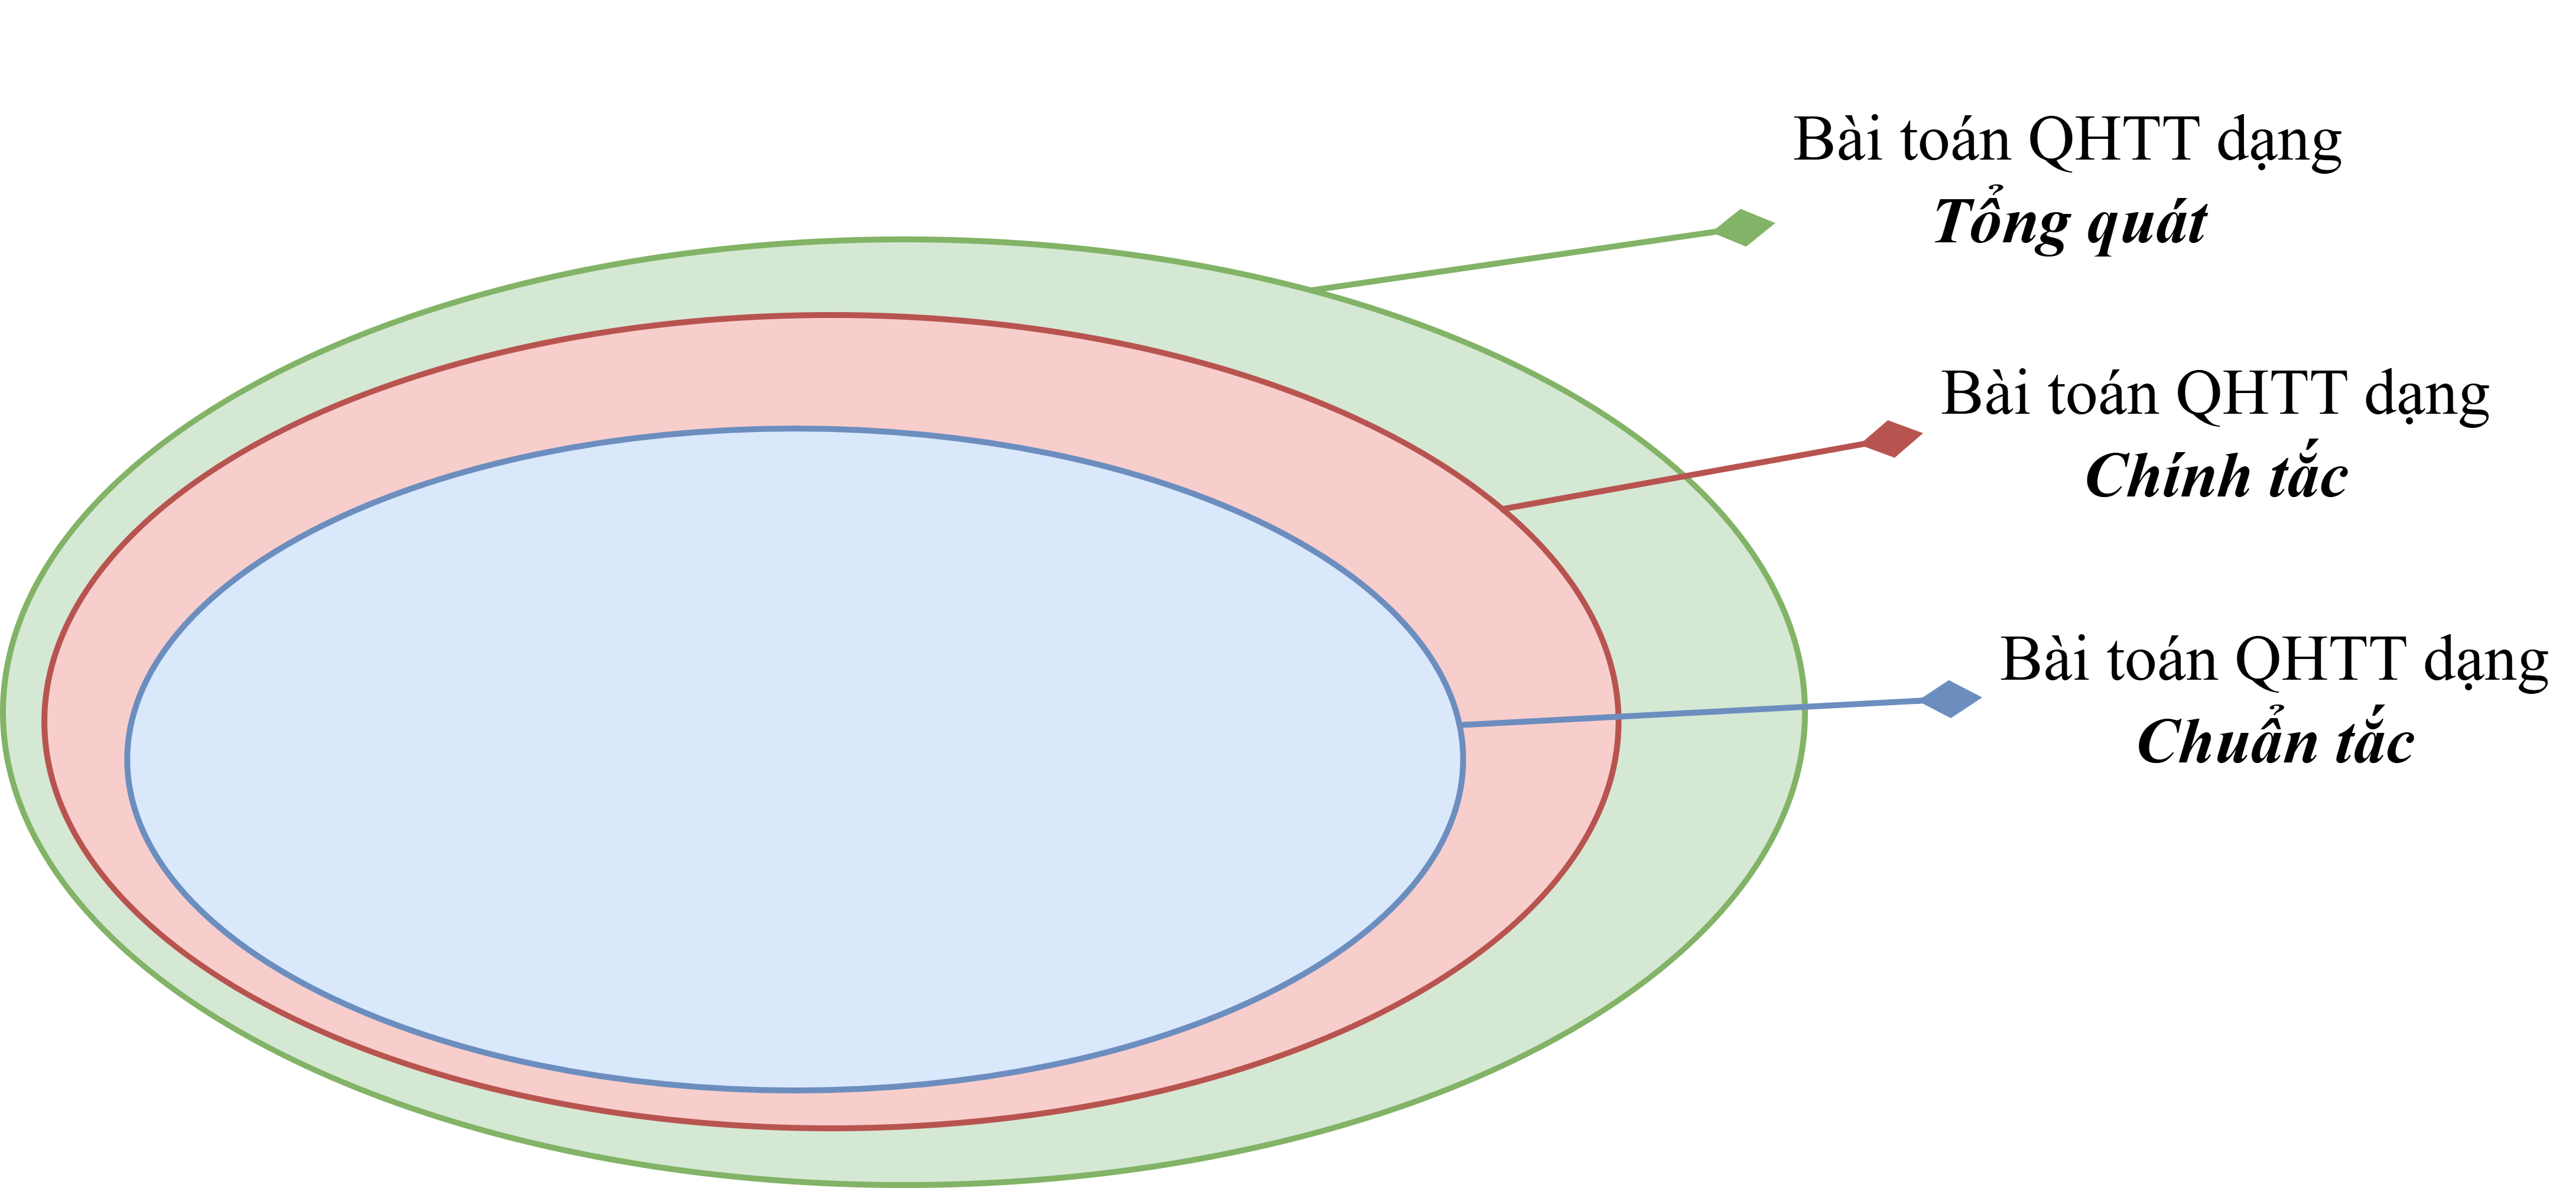
\includegraphics[width=1\linewidth]{images/Graphic.drawio.png}
    \caption{Sơ đồ phân loại 3 dạng bài toán QHTT}
    \label{fig:phanloai_qhtt}
\end{figure}

\subsection{Bài toán QHTT tổng quát}
Từ các bài toán thực tế, ta có thể tổng quát hóa mô hình toán học của một bài toán Quy hoạch tuyến tính (QHTT) dưới dạng sau:

\textbf{Hàm mục tiêu:}
\begin{formula}
    Z = \sum_{j=1}^{n} c_j x_j \rightarrow \max (\text{hoặc } \min)
\end{formula}

\textbf{Hệ ràng buộc chính:}
\begin{formula}
    \sum_{j=1}^{n} a_{ij} x_j 
    \begin{bmatrix} 
        \ge \\ 
        \le \\ 
        = 
    \end{bmatrix} 
    b_i, \quad (i = \overline{1,m})
\end{formula}

\textbf{Ràng buộc dấu:}
\begin{formula}
    x_j 
    \begin{bmatrix} 
        \ge 0 \\ 
        \le 0 \\ 
        \text{tùy ý} 
    \end{bmatrix}, \quad (j = \overline{1,n})
\end{formula}

Trong đó:
\begin{itemize}
    \item $x_j$: Các biến quyết định (ẩn số cần tìm).
    \item $c_j$: Các hệ số của hàm mục tiêu.
    \item $a_{ij}$: Các hệ số công nghệ (nằm ở dòng $i$, cột $j$).
    \item $b_i$: Giá trị giới hạn vế phải của các ràng buộc.
\end{itemize}

\subsection{Tính chất cốt lõi của bài toán QHTT}
Dựa trên các khái niệm về phương án, một bài toán QHTT luôn tuân theo các tính chất toán học sau:
\begin{itemize}
    \item Nếu bài toán tìm Max (hoặc Min) có tập phương án không rỗng và hàm mục tiêu bị chặn trên (hoặc chặn dưới), thì bài toán chắc chắn có phương án tối ưu.
    \item Nếu bài toán QHTT có nhiều hơn một PATƯ thì nó sẽ có vô số PATƯ. 
    \item \textbf{Cụ thể:} Nếu $x^0$ và $x^1$ là hai phương án tối ưu phân biệt, thì mọi bao lồi (tổ hợp lồi) của chúng có dạng:
    \begin{equation*}
        x = \alpha x^0 + (1-\alpha)x^1, \quad \text{với } \alpha \in
    \end{equation*}
    cũng là một phương án tối ưu của bài toán này.
\end{itemize}


Để thuận lợi cho việc áp dụng các thuật toán giải quyết trên máy tính, từ bài toán tổng quát, người ta phân loại và biến đổi mô hình về 3 dạng đặc biệt sau:

\subsection{Bài toán QHTT dạng chính tắc}
Bài toán QHTT dạng chính tắc là bài toán có tất cả các ràng buộc chính ở dạng đẳng thức ($=$) và mọi ràng buộc dấu đều không âm ($x_j \ge 0$).

Mô hình toán học có dạng:
\begin{formula}
    \begin{aligned}
    Z = \sum_{j=1}^{n} c_j x_j \rightarrow \max (\text{hoặc } \min) \\
    \sum_{j=1}^{n} a_{ij} x_j = b_i, \quad (i = \overline{1,m}) \\
    x_j \ge 0, \quad (j = \overline{1,n})
    \end{aligned}
\end{formula}


\textbf{Ma trận điều kiện:} Ma trận $A = (a_{ij})$ chứa các hệ số của hệ ràng buộc chính được gọi là ma trận điều kiện. Cột thứ $j$ của ma trận $A$ (ký hiệu $A_j$) được gọi là vector điều kiện của biến $x_j$.

\subsection{Bài toán QHTT dạng chuẩn}
Bài toán QHTT được gọi là có dạng chuẩn nếu nó đã ở dạng chính tắc, vế phải của các ràng buộc không âm ($b_i \ge 0$) và \textbf{mỗi ràng buộc chính phải có một biến cơ sở}.

\textit{Biến cơ sở} ứng với một phương trình ràng buộc là biến có hệ số bằng 1 ở phương trình đó và có hệ số bằng 0 ở tất cả các phương trình còn lại.

Mô hình dạng chuẩn được viết phân tách như sau:

\begin{formula}
\begin{alignedat}{4}
    Z = & \sum_{j=1}^{n} c_j x_j & \rightarrow \max (\text{hoặc } \min) \\
    \text{s.t.} \quad & x_1 + a_{1, m+1}x_{m+1} + \dots + a_{1n}x_n & = b_1 \\
    & x_2 + a_{2, m+1}x_{m+1} + \dots + a_{2n}x_n & = b_2 \\
    & \dots \\
    & x_m + a_{m, m+1}x_{m+1} + \dots + a_{mn}x_n & = b_m \\
    & \rlap{$x_j \ge 0, \quad b_i \ge 0$}
\end{alignedat}    
\end{formula}

Trong mô hình trên, các biến $x_1, x_2, \dots, x_m$ đóng vai trò là các biến cơ sở, trong khi $x_{m+1}, \dots, x_n$ là các biến không cơ sở.

\subsection{Kỹ thuật biến đổi mô hình QHTT}
Để áp dụng được thuật toán Đơn hình, mọi bài toán QHTT đều phải được đưa về dạng Chuẩn tắc. Dưới đây là các phép biến đổi cơ bản:

\textbf{1. Biến đổi Ràng buộc chính (Đưa về dấu $=$):}
\begin{itemize}
    \item Nếu ràng buộc thứ $i$ có dấu "$\le$": Ta \textbf{cộng thêm} một \textit{biến phụ} $x_{n+i} \ge 0$ vào vế trái.
    \item Nếu ràng buộc thứ $i$ có dấu "$\ge$": Ta \textbf{trừ đi} một \textit{biến phụ} $x_{n+i} \ge 0$ ở vế trái.
    \item Nếu phương trình thiếu biến cơ sở: Ta \textbf{cộng thêm} một \textit{biến giả} vào vế trái (Kèm theo việc thêm hệ số phạt $\pm M$ trên hàm mục tiêu).
\end{itemize}

\textbf{2. Biến đổi Ràng buộc dấu (Đưa về $\ge 0$):}
\begin{itemize}
    \item Nếu biến $x_j \le 0$: Đặt biến mới $x'_j = -x_j$, khi đó $x'_j \ge 0$. Thay thế $-x'_j$ vào mọi vị trí của $x_j$ trong bài toán.
    \item Nếu biến $x_j$ \textbf{tùy ý} (không ràng buộc dấu): Đặt $x_j = x_j^+ - x_j^-$, với điều kiện $x_j^+, x_j^- \ge 0$.
\end{itemize}


\vspace{0.5cm}
\begin{figure}[H]
    \centering
    \resizebox{\textwidth}{!}{
    \begin{tikzpicture}[
        node distance=2.5cm, % Thu hẹp khoảng cách giữa các hộp một chút
        box/.style={rectangle, rounded corners=8pt, thick, align=left, inner sep=8pt, drop shadow={opacity=0.1}},
        arrow/.style={->, >=stealth, line width=1.5pt}
    ]

    % ==========================================
    % KHỐI 1: TỔNG QUÁT
    % ==========================================
    \node[box, fill=blue!5, draw=blue!80!black] (tongquat) {
        \renewcommand{\arraystretch}{1.6}
        % Chỉnh độ rộng cột nhỏ lại để không bị tràn lề
        \begin{tabular}{p{7cm} | p{6.5cm}}
            \textbf{\Large 1. Dạng Tổng Quát} & \textbf{\Large Mô hình Toán học} \\[0.1cm]
            $\bullet$ \textbf{Hàm mục tiêu:} $Z \rightarrow \max$ hoặc $\min$ & 
            $\displaystyle Z = \sum_{j=1}^n c_j x_j \rightarrow \max (\min)$ \\
            $\bullet$ \textbf{Ràng buộc chính:} Có thể chứa $\le, \ge$ hoặc $=$ & 
            % Dàn phẳng các dấu để không bị giãn chiều cao
            $\displaystyle \sum_{j=1}^n a_{ij} x_j \in \{\le, \ge, =\} \, b_i$ \\
            $\bullet$ \textbf{Ràng buộc dấu:} $x_j \ge 0, \le 0$ hoặc tùy ý & 
            $\displaystyle x_j \in \{\ge 0, \le 0, \text{tùy ý}\}$
        \end{tabular}
    };

    % ==========================================
    % KHỐI 2: CHÍNH TẮC
    % ==========================================
    \node[box, fill=green!5, draw=green!60!black, below=2.5cm of tongquat] (chinhtac) {
        \renewcommand{\arraystretch}{1.6}
        \begin{tabular}{p{7cm} | p{6.5cm}}
            \textbf{\Large 2. Dạng Chính Tắc} & \textbf{\Large Mô hình Toán học} \\[0.1cm]
            $\bullet$ \textbf{Hàm mục tiêu:} $Z \rightarrow \max$ hoặc $\min$ & 
            $\displaystyle Z = \sum_{j=1}^n c_j x_j \rightarrow \max (\min)$ \\
            $\bullet$ \textbf{Ràng buộc chính:} \textcolor{red}{\textbf{Bắt buộc là dấu $=$}} & 
            $\displaystyle \sum_{j=1}^n a_{ij} x_j \;\textcolor{red}{=}\; b_i$ \\
            $\bullet$ \textbf{Ràng buộc dấu:} \textcolor{red}{\textbf{Mọi biến $x_j \ge 0$}} & 
            $\displaystyle x_j \;\textcolor{red}{\ge 0}$
        \end{tabular}
    };

    % ==========================================
    % KHỐI 3: CHUẨN TẮC
    % ==========================================
    \node[box, fill=orange!5, draw=orange!80!black, below=2.5cm of chinhtac] (chuantac) {
        \renewcommand{\arraystretch}{1.6}
        \begin{tabular}{p{7cm} | p{6.5cm}}
            \textbf{\Large 3. Dạng Chuẩn Tắc} & \textbf{\Large Mô hình Toán học} \\[0.1cm]
            $\bullet$ \textbf{Hàm mục tiêu:} $Z \rightarrow \max$ hoặc $\min$ & 
            $\displaystyle Z = \sum_{j=1}^n c_j x_j \rightarrow \max (\min)$ \\
            $\bullet$ \textbf{Ràng buộc \& Vế phải:} Dấu $=$ và \textcolor{red}{\textbf{$b_i \ge 0$}} & 
            $\displaystyle \sum_{j=1}^n a_{ij} x_j = b_i \quad (\textcolor{red}{b_i \ge 0})$ \\
            $\bullet$ \textbf{Cơ sở:} \textcolor{red}{\textbf{Đủ $m$ biến cơ sở}} (Ma trận $I_m$) & 
            $\displaystyle \textcolor{red}{x_i} + \sum_{k=m+1}^n a_{ik} x_k = b_i$ \\
            $\bullet$ \textbf{Ràng buộc dấu:} Mọi biến $x_j \ge 0$ & 
            $\displaystyle x_j \ge 0$
        \end{tabular}
    };

    % ==========================================
    % MŨI TÊN VÀ TEXT GIẢI THÍCH
    % ==========================================
    
    % Từ Tổng quát -> Chính tắc
    \draw[arrow, blue!80!black] (tongquat.south) -- (chinhtac.north) 
        node[midway, fill=white, draw=blue!80!black, thick, rounded corners, align=center, inner sep=6pt, drop shadow={opacity=0.1}] {
            \textbf{\textcolor{blue!80!black}{Bước 1: Khử bất phương trình \& Dấu âm}}\\
            $\le$ thì \textbf{cộng} biến phụ \quad $\Big|$ \quad $\ge$ thì \textbf{trừ} biến phụ \\
            $x_j \le 0 \Rightarrow$ Đặt $x'_j = -x_j$ \quad $\Big|$ \quad $x_j$ tùy ý $\Rightarrow$ Đặt $x_j = x'_j - x''_j$
        };

    % Từ Chính tắc -> Chuẩn tắc
    \draw[arrow, green!60!black] (chinhtac.south) -- (chuantac.north) 
        node[midway, fill=white, draw=green!60!black, thick, rounded corners, align=center, inner sep=6pt, drop shadow={opacity=0.1}] {
            \textbf{\textcolor{green!60!black}{Bước 2: Chuẩn bị cơ sở cho thuật toán}}\\
            $b_i < 0 \Rightarrow$ Nhân cả 2 vế phương trình với $(-1)$ \\
            Thiếu biến cơ sở $\Rightarrow$ Cộng \textbf{biến giả} (Kèm theo thêm $\pm M$ vào $Z$)
        };

    \end{tikzpicture}
    }
    \caption{Sơ đồ đối chiếu lý thuyết và ký hiệu toán học qua các dạng bài toán}
    \label{fig:flowchart_forms}
\end{figure}

\subsection{Bài toán QHTT tương đương}
Trong nhiều trường hợp tính toán, việc chuyển đổi qua lại giữa bài toán tìm lớn nhất (Max) và nhỏ nhất (Min) là cần thiết. Hai bài toán QHTT được gọi là tương đương với nhau khi chúng có chung tập phương án và phương án tối ưu.

Giả sử ta có bài toán gốc tìm Max:
\begin{equation*}
    (P): \quad Z = \sum_{j=1}^{n} c_j x_j \rightarrow \max
\end{equation*}

Thì bài toán tương đương của nó sẽ là tìm Min của hàm đối:
\begin{equation*}
    (P'): \quad Z' = -Z = \sum_{j=1}^{n} (-c_j) x_j \rightarrow \min
\end{equation*}
Điều này có nghĩa là khi giải bài toán, thay vì tìm Max của hàm $Z$, ta có thể tìm Min của hàm $-Z$.

\section{Thuật toán Đơn hình mở rộng}



    \section{Phương pháp hình học}

Phương pháp hình học là một công cụ trực quan và cực kỳ hiệu quả để giải quyết các bài toán QHTT có \textbf{hai biến số}. Mặc dù không thể áp dụng cho các bài toán có từ ba biến trở lên (do giới hạn của không gian vẽ hình), phương pháp này lại là nền tảng tuyệt vời nhất để người học có thể "nhìn thấy" bản chất của quá trình tối ưu hóa.

Để giải một bài toán QHTT bằng phương pháp hình học, ta thực hiện theo 3 bước chuẩn mực sau:

\subsubsection{Các bước thực hiện thuật toán}

\textbf{Bước 1: Vẽ tập phương án của bài toán ($\Omega$)}
\begin{itemize}
    \item Lần lượt vẽ các đường thẳng ứng với \textit{dấu bằng} ($=$) của các hệ thức ràng buộc lên mặt phẳng tọa độ $Ox_1x_2$.
    \item Lựa chọn các nửa mặt phẳng thỏa mãn từng bất phương trình ràng buộc (bằng cách thử tọa độ điểm gốc $O(0,0)$ hoặc một điểm bất kỳ).
    \item Phần không gian giao nhau (phần chung) của tất cả các nửa mặt phẳng này chính là \textbf{tập phương án} của bài toán (ký hiệu là $\Omega$).
\end{itemize}

\textbf{Bước 2: Vẽ đường mức $\Delta$ (Đường hàm mục tiêu)}
\begin{itemize}
    \item Chọn một điểm $(x_1^0, x_2^0)$ bất kỳ nằm trong miền $\Omega$ và thay vào hàm mục tiêu $Z = c_1x_1 + c_2x_2$ để tìm ra một giá trị $Z_0$ cụ thể.
    \item Vẽ đường thẳng $\Delta$ có phương trình: $c_1x_1 + c_2x_2 = Z_0$.
    \item Xác định \textbf{vector pháp tuyến} $\vec{n} = (c_1, c_2)$ của đường $\Delta$. Đặc điểm của vector này là nó luôn chỉ về hướng làm cho hàm mục tiêu $Z$ \textbf{tăng lên}.
\end{itemize}

\textbf{Bước 3: Xác định lời giải bài toán (Tịnh tiến đường mức)}
Bạn hãy tưởng tượng đường mức $\Delta$ như một chiếc thước kẻ. Cầm chiếc thước này và tịnh tiến nó song song theo hướng của vector pháp tuyến $\vec{n}$ (nếu bài toán tìm Max) hoặc tịnh tiến ngược hướng $\vec{n}$ (nếu bài toán tìm Min):
\begin{itemize}
    \item Nếu đường $\Delta$ đạt đến một \textbf{vị trí tới hạn} (là điểm cuối cùng nó chạm vào miền $\Omega$ trước khi rời hẳn ra ngoài) và toàn bộ miền $\Omega$ nằm về một phía của $\Delta$, thì điểm chạm đó chính là \textbf{Phương án tối ưu}.
    \item Nếu $\Delta$ cứ tịnh tiến mãi mà vẫn luôn cắt miền $\Omega$ (không có điểm dừng cuối cùng), ta kết luận hàm mục tiêu không bị chặn và bài toán \textbf{không có lời giải} [2, 4, 7].
\end{itemize}

\subsubsection{Phương pháp thay thế nhanh: Đánh giá qua các đỉnh}
Nếu sau khi vẽ hình ở Bước 1, bạn nhận thấy tập phương án $\Omega$ là một \textbf{đa giác lồi giới nội} (một hình khép kín, bị chặn ở mọi phía), bạn có thể bỏ qua Bước 2 và Bước 3 để áp dụng một quy tắc cực kỳ đơn giản sau:

\begin{enumerate}
    \item Vì đa giác giới nội luôn có số lượng đỉnh hữu hạn, và mỗi đỉnh chính là một Phương án cơ bản (PACB), bạn chỉ cần tìm chính xác \textbf{tọa độ của tất cả các đỉnh} này [4, 5, 7].
    \item Lần lượt thay tọa độ của từng đỉnh vào hàm mục tiêu $Z$.
    \item \textbf{Kết luận:} So sánh các kết quả vừa tính. Phương án nào cho giá trị $Z$ lớn nhất (với bài Max) hoặc nhỏ nhất (với bài Min) thì đó chính là \textbf{Phương án tối ưu} của bài toán.
\end{enumerate}

\subsubsection{Một số chú ý quan trọng cần ghi nhớ}
\begin{itemize}
    \item \textbf{Tập phương án đa dạng:} Miền $\Omega$ có thể là tập rỗng (bài toán vô nghiệm), chỉ là một điểm duy nhất, là đa giác lồi bị chặn (như hình bình hành, tam giác) hoặc đa giác lồi không giới nội (kéo dài vô tận về một hướng).
    \item \textbf{Bản chất của điểm tối ưu:} Nếu miền $\Omega$ là một tập lồi đa diện, lời giải tối ưu của bài toán (nếu có) \textbf{chắc chắn sẽ đạt được tại ít nhất một đỉnh} của miền đó.
    \item \textbf{Vô số nghiệm:} Nếu trong quá trình tịnh tiến (Bước 3), đường mức $\Delta$ ở vị trí tới hạn lại hoàn toàn trùng khớp với một cạnh của đa giác $\Omega$, thì bài toán sẽ có \textbf{vô số phương án tối ưu}. Khi đó, mọi điểm nằm trên đoạn thẳng (cạnh) đó đều là lời giải xuất sắc nhất.
\end{itemize}

\vspace{0.5cm}
\textbf{Minh họa bằng đồ thị:}
\begin{figure}[htbp]
    \centering
    \begin{tikzpicture}[scale=1.2, >=stealth]
        % Tô màu miền phương án \Omega trước để nằm dưới các nét vẽ
        \fill[cyan!15] (0,2) -- (2,4) -- (4,2) -- (3,0) -- (0,0) -- cycle;

        % Vẽ hệ trục tọa độ
        \draw[->, thick] (-1,0) -- (6,0) node[right] {$x_1$};
        \draw[->, thick] (0,-1) -- (0,5) node[above] {$x_2$};
        \node[below left] at (0,0) {$O$};

        % Vẽ các đường thẳng ràng buộc (viền của tập phương án)
        \draw[thick, blue] (-1,1) -- (5,7) node[right] {$(d_1)$}; 
        \draw[thick, red] (1,5) -- (5,1) node[right] {$(d_2)$};
        \draw[thick, green!60!black] (4.5,-1.5) -- (2.5,4.5) node[above] {$(d_3)$};

        % Đánh dấu các đỉnh của đa giác \Omega
        \filldraw (0,2) circle (1.5pt) node[left] {$A$};
        \filldraw (2,4) circle (1.5pt) node[above] {$B$};
        \filldraw (4,2) circle (1.5pt) node[right] {$C$};
        \filldraw (3,0) circle (1.5pt) node[below] {$D$};
        \node at (2,1.5) {\Large $\Omega$};

        % Vẽ đường mức \Delta và vector pháp tuyến n
        \draw[dashed, thick, orange] (-1,3) -- (5,-0.5) node[below] {$\Delta$ (Đường mức)};
        \draw[->, very thick, orange] (2,1.25) -- (2.8, 2.6) node[above right] {$\vec{n}$};

        % Vẽ đường mức tới hạn tại đỉnh B (PATƯ)
        \draw[dashed, thick, orange!70!black] (0.5,4.8) -- (5,2.2) node[right] {$\Delta_{max}$};
        \filldraw[orange!70!black] (2,4) circle (2pt);
    \end{tikzpicture}
    \caption{Minh họa tập phương án $\Omega$ và sự tịnh tiến đường mức $\Delta$ tìm đỉnh tối ưu}
    \label{fig:phuongphap_hinhhoc}
\end{figure}

\textit{Giải thích hình vẽ:} Trong hình trên, vùng màu xanh là tập phương án $\Omega$ hợp lệ. Đường mức $\Delta$ (nét đứt) được tịnh tiến song song theo hướng của vector pháp tuyến $\vec{n}$. Điểm cuối cùng mà $\Delta$ chạm vào miền $\Omega$ trước khi rời ra ngoài chính là đỉnh $B$. Do đó, $B$ là Phương án tối ưu của bài toán.

    
\chapter{Thuật toán Đơn hình}
    \section{Thuật toán đơn hình (Simplex Method)}

\subsection{Ý tưởng của thuật toán}
Thuật toán đơn hình là phương pháp đại số lặp để giải bài toán QHTT. 
Xuất phát từ một phương án cơ bản (PACB) $x^0$, ta tìm cách đánh giá xem $x^0$ đã là phương án tối ưu (PATƯ) chưa. Nếu chưa, ta xây dựng một PACB mới $x^1$ tốt hơn và tiếp tục đánh giá. Quá trình này được lặp lại (mỗi lần lặp là một phép biến đổi Gauss - Jordan) cho đến khi tìm được PATƯ hoặc phát hiện ra bài toán không có lời giải.

\textbf{Yêu cầu đầu vào:} Để đơn giản hóa quá trình, thuật toán đơn hình yêu cầu mô hình bài toán QHTT phải được đưa về \textbf{dạng chuẩn} (có sẵn các biến cơ sở).

\subsection{Các bước thực hiện thuật toán}

\textbf{Bước 1: Xây dựng PACB xuất phát} \\
Cho tất cả các biến không cơ sở bằng $0$. Khi đó, các biến cơ sở sẽ nhận giá trị bằng đúng vế phải của hệ ràng buộc: $x_i = b_i \quad (i = \overline{1,m})$. \\
Giá trị hàm mục tiêu xuất phát là: $Z_0 = \sum_{i=1}^{m} C_i b_i$.

\vspace{0.3cm}
\textbf{Bước 2: Xây dựng tiêu chuẩn tối ưu} \\
Tính các \textbf{hệ số ước lượng} $\Delta_j$ cho từng biến $x_j$ theo công thức:
\begin{formula}
    \Delta_j = \sum_{i=1}^{m} C_i a_{ij} - c_j
\end{formula}
\textit{(Chú ý: Đối với các biến đang nằm trong cơ sở, ta luôn có $\Delta_j = 0$).}

Dựa vào giá trị $\Delta_j$, tiêu chuẩn tối ưu được phát biểu như sau:
\begin{itemize}
    \item \textbf{Đối với bài toán tìm Max}:
    \begin{itemize}
        \item Nếu $\Delta_j \ge 0, \forall j$ thì PACB hiện hành là tối ưu.
        \item Nếu $\exists k$ sao cho $\Delta_k < 0$ thì PACB hiện hành chưa tối ưu (cần thực hiện Bước 3).
    \end{itemize}
    \item \textbf{Đối với bài toán tìm Min}:
    \begin{itemize}
        \item Nếu $\Delta_j \le 0, \forall j$ thì PACB hiện hành là tối ưu.
        \item Nếu $\exists k$ sao cho $\Delta_k > 0$ thì PACB hiện hành chưa tối ưu.
    \end{itemize}
\end{itemize}

\subsubsection*{Mẹo tính nhanh: Quy tắc ``chữ L ngược''}

Để tránh nhầm lẫn khi tính $\Delta_j$ theo công thức gốc, ta có thể hình dung phép tính dưới dạng đồ họa sơ đồ sau. Các phép nhân được thực hiện theo chiều dọc từ trên xuống, sau đó trừ đi hệ số trên cùng:

\begin{figure}[H]
    \centering
    \begin{tikzpicture}[
        node distance=0.8cm and 2cm,
        cell/.style={rectangle, draw, thick, minimum width=1.5cm, minimum height=0.8cm, align=center},
        highlight/.style={fill=blue!10, draw=blue, thick},
        target/.style={fill=red!10, draw=red, thick},
        arrow/.style={->, >=stealth, thick, blue}
    ]

    \node (cb_title) {\textbf{Cột $\mathbf{C_b}$}};
    \node[cell, highlight, below=0.2cm of cb_title] (cb1) {$C_1$};
    \node[cell, highlight, below=of cb1] (cb2) {$C_2$};
    \node[below=0.4cm of cb2] (cb_dots) {$\vdots$};
    \node[cell, highlight, below=0.4cm of cb_dots] (cbm) {$C_m$};

    \node[right=3cm of cb_title] (xj_title) {\textbf{Cột $\mathbf{x_j}$}};
    \node[cell, target, below=0.2cm of xj_title, label=right:\textcolor{red}{$- c_j$ (Trừ đi)}] (cj) {$c_j$};
    \node[cell, highlight, below=0.8cm of cj] (a1j) {$a_{1j}$};
    \node[cell, highlight, below=of a1j] (a2j) {$a_{2j}$};
    \node[below=0.4cm of a2j] (aj_dots) {$\vdots$};
    \node[cell, highlight, below=0.4cm of aj_dots] (amj) {$a_{mj}$};

    \node[cell, fill=green!15, draw=green!60!black, thick, below=0.8cm of amj] (deltaj) {$\mathbf{\Delta_j}$};

    \draw[arrow] (cb1.east) -- node[above] {$\times$} (a1j.west);
    \draw[arrow] (cb2.east) -- node[above] {$\times$} (a2j.west);
    \draw[arrow] (cbm.east) -- node[above] {$\times$} (amj.west);

    \draw[->, >=stealth, thick, red] (cj.west) to[out=180, in=180] node[left] {Trừ đi (-)} (deltaj.west);

    \draw[dashed, blue, thick, rounded corners]
        ([xshift=-0.5cm, yshift=0.3cm]cb1.north west) rectangle
        ([xshift=0.5cm, yshift=-0.3cm]amj.south east);

    \node[right=1.5cm of a2j, text=blue, align=left] {\textbf{Bước 1:}\\Tính tổng các\\tích vô hướng ($\Sigma$)};
    \node[right=1.5cm of deltaj, text=black, align=left] {\textbf{Bước 2:}\\Ghi kết quả vào $\Delta_j$};

    \end{tikzpicture}
    \caption{Trực quan hóa cách tính hệ số ước lượng $\Delta_j$}
\end{figure}

\subsubsection*{Ví dụ minh họa: Tính $\Delta_2$ tại Bảng đơn hình 2}

Dưới đây là sơ đồ minh họa cách tính $\Delta_2$ ở Bảng đơn hình 2 (được trích từ bài toán ở phần Sample Test).
Ta có cột hệ số cơ sở $\mathbf{C_b} = (0, 15, 0)^T$, cột $\mathbf{x_2} = (-4, 2, -3)^T$ và hệ số hàm mục tiêu $c_2 = 9$.

\begin{figure}[H]
    \centering
    \begin{tikzpicture}[
        node distance=0.8cm and 2.5cm,
        cell/.style={rectangle, draw, thick, minimum width=1.5cm, minimum height=0.8cm, align=center},
        highlight/.style={fill=blue!10, draw=blue, thick},
        target/.style={fill=red!10, draw=red, thick},
        result/.style={fill=green!15, draw=green!60!black, thick},
        arrow/.style={->, >=stealth, thick, blue}
    ]

    \node (cb_title) {\textbf{Cột $\mathbf{C_b}$}};
    \node[cell, highlight, below=0.2cm of cb_title] (cb1) {$0$};
    \node[cell, highlight, below=0.5cm of cb1] (cb2) {$15$};
    \node[cell, highlight, below=0.5cm of cb2] (cb3) {$0$};

    \node[right=3cm of cb_title] (xj_title) {\textbf{Cột $\mathbf{x_2}$}};
    \node[cell, target, below=0.2cm of xj_title, label=right:\textcolor{red}{$- 9$ (Trừ đi $c_2$)}] (cj) {$9$};
    \node[cell, highlight, below=0.8cm of cj] (a1j) {$-4$};
    \node[cell, highlight, below=0.5cm of a1j] (a2j) {$2$};
    \node[cell, highlight, below=0.5cm of a2j] (a3j) {$-3$};

    \node[cell, result, below=0.8cm of a3j] (deltaj) {$\mathbf{21}$};

    \draw[arrow] (cb1.east) -- node[above] {$\times$} (a1j.west);
    \draw[arrow] (cb2.east) -- node[above] {$\times$} (a2j.west);
    \draw[arrow] (cb3.east) -- node[above] {$\times$} (a3j.west);

    \draw[->, >=stealth, thick, red] (cj.west) to[out=180, in=180] node[left, align=center] {Trừ đi\\$(-)$} (deltaj.west);

    \draw[dashed, blue, thick, rounded corners]
        ([xshift=-0.5cm, yshift=0.3cm]cb1.north west) rectangle
        ([xshift=0.5cm, yshift=-0.3cm]a3j.south east);

    \node[right=1.5cm of a2j, text=blue, align=left] {\textbf{Bước 1: Tổng tích vô hướng ($\Sigma$)}\\$0 \times (-4) + 15 \times 2 + 0 \times (-3)$\\$= 0 + 30 + 0$\\$= \mathbf{30}$};
    \node[right=1.5cm of deltaj, text=black, align=left] {\textbf{Bước 2: Trừ đi $c_2$}\\$30 - 9 = \mathbf{21}$\\$\rightarrow \Delta_2 = 21$};

    \end{tikzpicture}
    \caption{Ví dụ thực tế: Tính $\Delta_2$ theo quy tắc ``Chữ L ngược''}
\end{figure}


\vspace{0.3cm}
\textbf{Bước 3: Xây dựng PACB mới tốt hơn (Quy tắc Dantzig)} \\
Để chuyển sang PACB mới, ta cần xác định một biến từ ngoài đưa \textbf{vào cơ sở} và một biến đang trong cơ sở bị đẩy \textbf{ra khỏi cơ sở}.
\begin{itemize}
    \item \textbf{Chọn biến vào cơ sở (Cột xoay):}
    \begin{itemize}
        \item \textit{Bài toán Max:} Chọn biến $x_k$ có $\Delta_k < 0$ và đạt giá trị âm nhỏ nhất (trị tuyệt đối lớn nhất).
        \item \textit{Bài toán Min:} Chọn biến $x_k$ có $\Delta_k > 0$ và đạt giá trị dương lớn nhất.
    \end{itemize}
    
    \item \textbf{Chọn biến ra khỏi cơ sở (Dòng xoay):} \\
    Lập tỷ số đơn hình $\lambda_i$ giữa cột phương án ($b_i$) và cột của biến vào cơ sở ($a_{ik}$) với điều kiện chỉ xét các $a_{ik} > 0$:
    \begin{formula}
        \lambda_i = \frac{b_i}{a_{ik}}, \quad \text{với } a_{ik} > 0
    \end{formula}
    Chọn biến cơ sở có tỷ số $\lambda_i$ \textbf{nhỏ nhất} (Min $\lambda$) để đưa ra khỏi cơ sở.
\end{itemize}

Phần tử nằm ở giao điểm của dòng xoay và cột xoay ($a_{ik}$) được gọi là \textbf{phần tử trụ} (hay phần tử chốt). Nếu có $\Delta_k$ vi phạm tiêu chuẩn tối ưu nhưng tất cả các $a_{ik} \le 0$, ta kết luận ngay bài toán không có lời giải (hàm mục tiêu không bị chặn).

\vspace{0.3cm}
\textbf{Bước 4: Xoay bảng (Biến đổi Gauss - Jordan)} \\
Lập bảng đơn hình mới dựa trên phần tử trụ vừa tìm được bằng phép biến đổi Gauss - Jordan:
\begin{itemize}
    \item \textbf{Dòng xoay mới} = Dòng xoay cũ chia cho phần tử trụ.
    \item \textbf{Các dòng khác mới} = Dòng cũ tương ứng $-$ (Hệ số ở cột xoay của dòng đó $\times$ Dòng xoay mới).
\end{itemize}
Sau khi tính xong bảng mới, ta quay lại \textbf{Bước 2} để kiểm tra tiêu chuẩn tối ưu cho đến khi thuật toán dừng lại.

\subsection{Sơ đồ và Cấu trúc Bảng đơn hình}

Để tiện cho việc tính toán và theo dõi các bước lặp, thuật toán đơn hình thường được trình bày dưới dạng bảng. Dưới đây là sơ đồ tổng quát của một bảng đơn hình cơ bản:

\begin{table}[htbp]
    \centering
    \renewcommand{\arraystretch}{1.3}
    \begin{tabular}{|c|c|c|c|c|c|c|c|}
        \hline
        \multirow{2}{*}{\textbf{Cơ sở}} & \multirow{2}{*}{$\mathbf{C_b}$} & \multirow{2}{*}{\textbf{PA ($b_i$)}} & $x_1$ & $x_2$ & $\dots$ & $x_n$ & \multirow{2}{*}{\textbf{Tỷ số $\lambda$}} \\
        \cline{4-7}
        & & & $c_1$ & $c_2$ & $\dots$ & $c_n$ & \\
        \hline
        $x_1$ & $C_1$ & $b_1$ & $a_{11}$ & $a_{12}$ & $\dots$ & $a_{1n}$ & $\lambda_1$ \\
        \hline
        $x_2$ & $C_2$ & $b_2$ & $a_{21}$ & $a_{22}$ & $\dots$ & $a_{2n}$ & $\lambda_2$ \\
        \hline
        $\vdots$ & $\vdots$ & $\vdots$ & $\vdots$ & $\vdots$ & $\ddots$ & $\vdots$ & $\vdots$ \\
        \hline
        $x_m$ & $C_m$ & $b_m$ & $a_{m1}$ & $a_{m2}$ & $\dots$ & $a_{mn}$ & $\lambda_m$ \\
        \hline
        \multicolumn{2}{|c|}{$\Delta_j$} & $\mathbf{Z(x^0)}$ & $\Delta_1$ & $\Delta_2$ & $\dots$ & $\Delta_n$ & \\
        \hline
    \end{tabular}
    \caption{Sơ đồ cấu trúc tổng quát của Bảng đơn hình}
\end{table}

\vspace{0.5cm}
\subsection{Biểu diễn Bảng đơn hình dưới góc nhìn Ma trận khối}

Để hiểu sâu sắc bản chất của thuật toán Đơn hình, ta có thể gộp các con số rời rạc trong bảng thành các ma trận khối (Block Matrices). Giả sử tại một bước lặp bất kỳ, bài toán có ma trận hệ số $A$. Ta chia $A$ thành hai phần: 
\begin{itemize}
    \item $B$: Ma trận cơ sở (gồm các cột ứng với biến cơ sở hiện tại). Khả nghịch và có ma trận nghịch đảo là $B^{-1}$.
    \item $N$: Ma trận không cơ sở (gồm các cột ứng với biến ngoài cơ sở).
\end{itemize}
Tương tự, vector biến $X$ được chia thành $X_B$ và $X_N$; vector hệ số hàm mục tiêu $C$ được chia thành $C_B$ và $C_N$. 

Khi đó, toàn bộ Bảng đơn hình ở bất kỳ bước lặp nào cũng tuân theo cấu trúc ma trận khối tuyệt đẹp sau:

\begin{table}[H]
    \centering
    \renewcommand{\arraystretch}{2} % Giãn dòng cho ma trận dễ nhìn
    \begin{tabular}{|c|c|c|c|c|}
        \hline
        \multirow{2}{*}{\textbf{Cơ sở}} & \multirow{2}{*}{$\mathbf{C_b}$} & \multirow{2}{*}{\textbf{PA ($b$)}} & \textbf{Biến cơ sở} ($X_B$) & \textbf{Biến không cơ sở} ($X_N$) \\
        \cline{4-5}
        & & & $C_B$ & $C_N$ \\
        \hline
        $X_B$ & $C_B$ & $\mathbf{B^{-1}b}$ & $\mathbf{I}$ \textit{(Ma trận đơn vị)} & $\mathbf{B^{-1}N}$ \\
        \hline
        \multicolumn{2}{|c|}{$\Delta_j$} & $\mathbf{Z = C_B^T B^{-1}b}$ & $\mathbf{0}$ & $\mathbf{C_B^T B^{-1}N - C_N}$ \\
        \hline
    \end{tabular}
    \caption{Bảng đơn hình tổng quát dưới dạng ma trận khối}
    \label{tab:matrix_simplex}
\end{table}

\textbf{Những hệ quả rút ra từ góc nhìn Ma trận:}
\begin{enumerate}
    \item \textbf{Cột Phương án (PA):} Luôn được tính bằng $B^{-1}b$. Đây chính là lý do phép biến đổi Gauss-Jordan luôn cập nhật đúng giá trị của phương án mới.
    \item \textbf{Vùng hệ số công nghệ trung tâm:} Các cột của biến cơ sở luôn tạo thành ma trận đơn vị $I$ (gồm các số 1 trên đường chéo và 0 ở vị trí khác). Phần còn lại chính là $B^{-1}N$.
    \item \textbf{Dòng hệ số ước lượng ($\Delta_j$):} 
    \begin{itemize}
        \item Đối với các biến cơ sở: $\Delta_B = C_B^T I - C_B = 0$. (Điều này giải thích vì sao $\Delta_j$ của biến trong cơ sở \textbf{luôn luôn bằng 0}).
        \item Đối với các biến ngoài cơ sở: $\Delta_N = C_B^T (B^{-1}N) - C_N$. (Đây chính là công thức tính bằng vector $\Delta_j = C_b^T \times A_j - c_j$ mà ta thường dùng).
    \end{itemize}
\end{enumerate}

\textbf{Giải thích các thành phần trong bảng đơn hình:}
\begin{itemize}
    \item \textbf{Dòng thứ 1 ($x_j$):} Ghi danh sách tất cả các biến số của bài toán.
    \item \textbf{Dòng thứ 2 ($c_j$):} Ghi các hệ số của hàm mục tiêu tương ứng với từng biến $x_j$.
    \item \textbf{Cột Cơ sở:} Liệt kê các biến đang đóng vai trò là biến cơ sở trong phương án hiện tại.
    \item \textbf{Cột $\mathbf{C_b}$ (hay $c_i$):} Ghi hệ số hàm mục tiêu của các biến cơ sở đang nằm trong cột Cơ sở.
    \item \textbf{Cột PA ($b_i$):} Cột Phương Án, ghi giá trị vế phải ứng với các biến cơ sở (đây chính là giá trị của phương án cơ bản hiện hành).
    \item \textbf{Miền trung tâm ($a_{ij}$):} Chứa các hệ số công nghệ (hay các vector điều kiện) của hệ ràng buộc.
    \item \textbf{Cột Tỷ số $\lambda$:} Dùng để lập tỷ số đơn hình $\lambda_i = \frac{b_i}{a_{ik}}$ (với $a_{ik} > 0$) nhằm mục đích chọn biến ra khỏi cơ sở theo quy tắc Dantzig.
    \item \textbf{Dòng $\Delta_j$:} Ghi các hệ số ước lượng của từng biến $x_j$. Ô đầu tiên của dòng này (nằm dưới cột PA) là giá trị của hàm mục tiêu $Z(x^0)$ tại phương án cơ bản đang xét. Cách tính $\Delta_j$ là lấy tích vô hướng của cột $C_b$ với vector điều kiện $A_j$ của biến $x_j$, sau đó trừ đi hệ số $c_j$ của biến đó.
\end{itemize}

\subsubsection*{Ví dụ trực quan: Tách bài toán thành các ma trận}

Để thân thiện với việc in ấn đen trắng, ta sử dụng các đường viền khác nhau (nét đứt, nét chấm, viền đôi, khoanh hình oval) kết hợp mũi tên chỉ hướng để ánh xạ dữ liệu từ mô hình toán học vào các ma trận khối tương ứng:

\begin{figure}[H]
    \centering
    % Dùng resizebox để sơ đồ tự động thu vừa khổ giấy A4
    \resizebox{1\textwidth}{!}{
    \begin{tikzpicture}[
        >=stealth,
        every node/.style={align=center},
        groupN/.style={draw, thick, rounded corners=5pt},                 % Viền bo góc nét liền (N)
        groupCN/.style={draw, thick, dashed, rounded corners=2pt},        % Viền nét đứt (C_N)
        groupCB/.style={draw, thick, dotted, rounded corners=2pt},        % Viền nét chấm (C_B)
        groupB/.style={draw, thick, double, rounded corners=5pt},         % Viền đôi (B)
        groupb/.style={draw, thick, ellipse, inner sep=1pt}               % Hình Oval (b)
    ]
    
    % ==========================================
    % HÀNG 1: HÀM MỤC TIÊU & MA TRẬN C
    % ==========================================
    \node (Z) at (-4, 3) {$Z \quad =$};
    \node[groupCN, label={[font=\bfseries]above:Hệ số ngoài cơ sở ($C_N$)}] (CN) at (-1, 3) {$11x_1 + 9x_2 + 15x_3$};
    \node (plus1) at (1.3, 3) {$+$};
    \node[groupCB, label={[font=\bfseries]above:Hệ số cơ sở ($C_B$)}] (CB) at (3.5, 3) {$0x_4 + 0x_5 + 0x_6$};
    \node (max) at (6, 3) {$\rightarrow \max$};
    
    \node (MatC) at (11, 3) {
        $\mathbf{C} = \Big( \underbrace{11 \quad 9 \quad 15}_{C_N} \quad \Big| \quad \underbrace{0 \quad 0 \quad 0}_{C_B} \Big)$
    };
    
    % Mũi tên hàng 1 (uốn vòng xuống dưới)
    \draw[->, thick, dashed] (CN.south) to[out=270, in=270, looseness=0.8] (9.5, 2.6);
    \draw[->, thick, dotted] (CB.south) to[out=270, in=270, looseness=0.8] (12.5, 2.6);
    
    % ==========================================
    % HÀNG 2: RÀNG BUỘC & MA TRẬN A, b
    % ==========================================
    \node (st) at (-4, -1) {s.t.};
    
    \node[groupN, label={[font=\bfseries]below:Khối ngoài cơ sở ($N$)}] (N) at (-1, -1) {
        \renewcommand{\arraystretch}{1.2}
        \begin{tabular}{c}
        $5x_1 + 4x_2 + 4x_3$ \\
        $3x_1 + 6x_2 + 3x_3$ \\
        $3x_1 + 7x_2 + 5x_3$
        \end{tabular}
    };
    
    \node (plus2) at (1.3, -1) {
        \renewcommand{\arraystretch}{1.2}
        \begin{tabular}{c} $+$ \\ $+$ \\ $+$ \end{tabular}
    };
    
    \node[groupB, label={[font=\bfseries]below:Khối cơ sở ($B$)}] (B) at (3.5, -1) {
        \renewcommand{\arraystretch}{1.2}
        \begin{tabular}{c}
        $1x_4 + 0x_5 + 0x_6$ \\
        $0x_4 + 1x_5 + 0x_6$ \\
        $0x_4 + 0x_5 + 1x_6$
        \end{tabular}
    };
    
    \node (eq) at (5.5, -1) {
        \renewcommand{\arraystretch}{1.2}
        \begin{tabular}{c} $=$ \\ $=$ \\ $=$ \end{tabular}
    };
    
    \node[groupb, label={[font=\bfseries]below:Vế phải ($b$)}] (b) at (7, -1) {
        \renewcommand{\arraystretch}{1.2}
        \begin{tabular}{c}
        $21000$ \\
        $15000$ \\
        $26000$
        \end{tabular}
    };
    
    \node (MatA) at (11.5, -1) {
        $\mathbf{A} = \left(
        \begin{array}{ccc | ccc}
            5 & 4 & 4 & 1 & 0 & 0 \\
            3 & 6 & 3 & 0 & 1 & 0 \\
            3 & 7 & 5 & 0 & 0 & 1
        \end{array}
        \right)$
    };
    
    \node (Matb) at (15.5, -1) {
        $\mathbf{b} = \begin{pmatrix} 21000 \\ 15000 \\ 26000 \end{pmatrix}$
    };
    
    % Mũi tên hàng 2 (uốn vòng xuống dưới)
    \draw[->, thick] (N.south) to[out=270, in=270, looseness=0.6] (10.5, -2.2);
    \draw[->, thick, double] (B.south) to[out=270, in=270, looseness=0.6] (12.8, -2.2);
    \draw[->, thick] (b.south) to[out=270, in=270, looseness=0.8] (Matb.south);
    
    \end{tikzpicture}
    }
    \caption{Ánh xạ từ Mô hình Toán học sang cấu trúc Ma trận (Bản in Trắng Đen)}
\end{figure}

\textbf{Nhận xét từ sơ đồ trên:}
\begin{itemize}[itemsep=0pt, parsep=0pt, topsep=5pt]
    \item \textbf{Khối cơ sở xuất phát ($B$):} Các biến phụ (được đóng khung viền kép) tạo thành ma trận cơ sở $\mathbf{B}$ và vector hệ số hàm mục tiêu $\mathbf{C_B}$ (viền chấm).
    \item \textbf{Khối ngoài cơ sở ($N$):} Các biến chính (khung viền đơn) sinh ra ma trận $\mathbf{N}$ và vector hệ số $\mathbf{C_N}$ (viền đứt).
    \item \textbf{Cột phương án ($b$):} Các con số sau dấu bằng (khoanh Oval) chính là vector vế phải $\mathbf{b}$.
    \item Lập Bảng đơn hình xuất phát thực chất là việc bê nguyên cụm ma trận $[\mathbf{A} \;|\; \mathbf{b}]$ và $[\mathbf{C}]$ đã được gom nhóm này đặt vào khung kẻ bảng.
\end{itemize}

\section{Sơ đồ lập bảng đơn hình}

\vspace{0.5cm}

\begin{figure}[H]
\centering
\resizebox{0.95\textwidth}{!}{
    \begin{tikzpicture}[
        node distance=1.2cm and 2cm,
        box/.style={rectangle, draw=black, thick, minimum width=4.5cm, minimum height=1.2cm, align=center, fill=blue!5, rounded corners=4pt, font=\normalsize},
        decision/.style={diamond, draw=orange!90!black, thick, minimum width=3cm, minimum height=3cm, align=center, fill=orange!10, aspect=1.8, font=\normalsize\bfseries},
        term/.style={rectangle, draw=green!60!black, thick, minimum width=3.5cm, minimum height=1.2cm, align=center, fill=green!10, rounded corners=4pt, font=\normalsize\bfseries},
        termbad/.style={rectangle, draw=red!60!black, thick, minimum width=3.5cm, minimum height=1.2cm, align=center, fill=red!10, rounded corners=4pt, font=\normalsize\bfseries},
        arrow/.style={->, >=stealth, thick, rounded corners=6pt}
    ]

    % --- CÁC KHỐI CHỨC NĂNG ---
    % Khối bắt đầu
    \node (start) [box, rounded corners=15pt, fill=black!10, draw=black, font=\normalsize\bfseries] {BẮT ĐẦU};
    
    % Khối khởi tạo
    \node (init) [box, below=0.8cm of start] {Lập bảng Đơn hình khởi tạo \&\\Tính các hệ số ước lượng $\Delta_j$};
    
    % Điều kiện tối ưu
    \node (check_opt) [decision, below=0.8cm of init] {$\forall \Delta_j \ge 0 \; ?$};
    \node (opt_found) [term, right=1.5cm of check_opt] {DỪNG THUẬT TOÁN\\Đã đạt Phương án tối ưu};
    
    % Chọn cột xoay
    \node (pivot_col) [box, below=0.8cm of check_opt] {Chọn cột xoay $k$ (Biến vào)\\($\Delta_k = \min \Delta_j < 0$)};
    
    % Điều kiện không giới hạn
    \node (check_bound) [decision, below=0.8cm of pivot_col] {$\forall a_{ik} \le 0 \; ?$};
    \node (unbounded) [termbad, right=1.5cm of check_bound] {DỪNG THUẬT TOÁN\\Bài toán không giới hạn\\(Hàm mục tiêu vô cực)};
    
    % Chọn hàng xoay
    \node (ratios) [box, below=0.8cm of check_bound] {Tính tỷ số $\lambda_i = \frac{b_i}{a_{ik}}$ (chỉ xét $a_{ik} > 0$)\\ Chọn hàng xoay $r$ (Biến ra): $\lambda_r = \min \lambda_i$};
    
    % Biến đổi Gauss
    \node (gauss) [box, left=2.5cm of pivot_col, fill=purple!5, draw=purple, thick] {Biến đổi Gauss-Jordan\\(Cập nhật lại bảng mới)};

    % --- CÁC ĐƯỜNG KẾT NỐI ---
    \draw[arrow] (start) -- (init);
    \draw[arrow] (init) -- (check_opt);
    
    % Nhánh kiểm tra tối ưu
    \draw[arrow] (check_opt) -- node[above, font=\footnotesize\bfseries, text=green!60!black] {ĐÚNG} (opt_found);
    \draw[arrow] (check_opt) -- node[right, font=\footnotesize\bfseries, text=red] {SAI (Chưa T.Ư)} (pivot_col);
    
    % Nhánh kiểm tra vô giới hạn
    \draw[arrow] (pivot_col) -- (check_bound);
    \draw[arrow] (check_bound) -- node[above, font=\footnotesize\bfseries, text=red] {ĐÚNG} (unbounded);
    \draw[arrow] (check_bound) -- node[right, font=\footnotesize\bfseries, text=green!60!black] {SAI} (ratios);
    
    % Vòng lặp xoay bảng
    \draw[arrow] (ratios.west) -| (gauss.south);
    \draw[arrow] (gauss.north) |- (init.west);

    \end{tikzpicture}
}
\caption{Sơ đồ thuật toán Đơn hình chi tiết cho bài toán quy hoạch tuyến tính (MAX)}
\end{figure}
\begin{figure}[H]
\centering
\resizebox{0.95\textwidth}{!}{
    \begin{tikzpicture}[
        node distance=1.2cm and 2cm,
        box/.style={rectangle, draw=black, thick, minimum width=4.5cm, minimum height=1.2cm, align=center, fill=blue!5, rounded corners=4pt, font=\normalsize},
        decision/.style={diamond, draw=orange!90!black, thick, minimum width=3cm, minimum height=3cm, align=center, fill=orange!10, aspect=1.8, font=\normalsize\bfseries},
        term/.style={rectangle, draw=green!60!black, thick, minimum width=3.5cm, minimum height=1.2cm, align=center, fill=green!10, rounded corners=4pt, font=\normalsize\bfseries},
        termbad/.style={rectangle, draw=red!60!black, thick, minimum width=3.5cm, minimum height=1.2cm, align=center, fill=red!10, rounded corners=4pt, font=\normalsize\bfseries},
        arrow/.style={->, >=stealth, thick, rounded corners=6pt}
    ]

    % --- CÁC KHỐI CHỨC NĂNG ---
    \node (start) [box, rounded corners=15pt, fill=black!10, draw=black, font=\normalsize\bfseries] {BẮT ĐẦU};
    
    \node (init) [box, below=0.8cm of start] {Lập bảng Đơn hình khởi tạo \&\\Tính các hệ số ước lượng $\Delta_j$};
    
    % Điều kiện tối ưu (Khác MAX)
    \node (check_opt) [decision, below=0.8cm of init] {$\forall \Delta_j \le 0 \; ?$};
    \node (opt_found) [term, right=1.5cm of check_opt] {DỪNG THUẬT TOÁN\\Đã đạt Phương án tối ưu};
    
    % Chọn cột xoay (Khác MAX)
    \node (pivot_col) [box, below=0.8cm of check_opt] {Chọn cột xoay $k$ (Biến vào)\\($\Delta_k = \max \Delta_j > 0$)};
    
    \node (check_bound) [decision, below=0.8cm of pivot_col] {$\forall a_{ik} \le 0 \; ?$};
    \node (unbounded) [termbad, right=1.5cm of check_bound] {DỪNG THUẬT TOÁN\\Bài toán không giới hạn\\(Hàm mục tiêu âm vô cực)};
    
    \node (ratios) [box, below=0.8cm of check_bound] {Tính tỷ số $\lambda_i = \frac{b_i}{a_{ik}}$ (chỉ xét $a_{ik} > 0$)\\ Chọn hàng xoay $r$ (Biến ra): $\lambda_r = \min \lambda_i$};
    
    \node (gauss) [box, left=2.5cm of pivot_col, fill=purple!5, draw=purple, thick] {Biến đổi Gauss-Jordan\\(Cập nhật lại bảng mới)};

    % --- CÁC ĐƯỜNG KẾT NỐI ---
    \draw[arrow] (start) -- (init);
    \draw[arrow] (init) -- (check_opt);
    
    \draw[arrow] (check_opt) -- node[above, font=\footnotesize\bfseries, text=green!60!black] {ĐÚNG} (opt_found);
    \draw[arrow] (check_opt) -- node[right, font=\footnotesize\bfseries, text=red] {SAI (Chưa T.Ư)} (pivot_col);
    
    \draw[arrow] (pivot_col) -- (check_bound);
    \draw[arrow] (check_bound) -- node[above, font=\footnotesize\bfseries, text=red] {ĐÚNG} (unbounded);
    \draw[arrow] (check_bound) -- node[right, font=\footnotesize\bfseries, text=green!60!black] {SAI} (ratios);
    
    \draw[arrow] (ratios.west) -| (gauss.south);
    \draw[arrow] (gauss.north) |- (init.west);

    \end{tikzpicture}
}
\caption{Sơ đồ thuật toán Đơn hình chi tiết cho bài toán quy hoạch tuyến tính (MIN)}
\end{figure}
    
\chapter{Bài toán Đối ngẫu}
    % \chapter{Bài toán đối ngẫu}

\section{Ý nghĩa và cách lập bài toán đối ngẫu}

\subsection{Ý nghĩa thực tế của bài toán đối ngẫu}
Trong thực tiễn kinh tế, mỗi bài toán Quy hoạch tuyến tính (gọi là bài toán gốc) luôn tồn tại song song một bài toán "anh em" với nó, được gọi là bài toán đối ngẫu. 

\begin{exampleblock}{Ví dụ minh họa}
Giả sử bạn là giám đốc của một công ty sản xuất (Công ty A) đang giải bài toán lập kế hoạch sản xuất tối ưu nhằm tối đa hóa lợi nhuận (tìm Max) dựa trên số lượng nguyên liệu giới hạn đang có trong kho [2]. Lúc này, một đối tác (Công ty B) đến đề nghị mua lại \textit{toàn bộ nguyên liệu} của bạn thay vì để bạn tự sản xuất [2].

Vấn đề đặt ra cho Công ty B là: \textit{Phải định giá mua mỗi đơn vị nguyên liệu là bao nhiêu để tổng chi phí mua là nhỏ nhất (tìm Min), nhưng vẫn đủ sức thuyết phục Công ty A bán lại (tức là giá mua nguyên liệu không được thấp hơn giá trị lợi nhuận mà Công ty A có thể tự làm ra)?} [2].

Bài toán định giá mua nguyên liệu của Công ty B chính là \textbf{Bài toán đối ngẫu} của bài toán sản xuất ban đầu [2].
\end{exampleblock}

\section{Quy tắc lập bài toán đối ngẫu}

Mối quan hệ chuyển đổi giữa bài toán gốc và bài toán đối ngẫu được thiết lập cực kỳ chặt chẽ. Một cách tổng quát, nếu bài toán gốc $(P)$ tìm giá trị lớn nhất (Max) thì bài toán đối ngẫu $(D)$ sẽ tìm giá trị nhỏ nhất (Min) và ngược lại [1]. 

Để thuận tiện cho việc lập mô hình, quy tắc chuyển đổi được tóm tắt qua hệ thống các bảng dưới đây:

\subsubsection{1. Bảng quy tắc tổng hợp bằng ký hiệu toán học}
Dưới đây là bảng ánh xạ 1-1 giữa các ràng buộc và biến số của hai bài toán được trình bày hoàn toàn bằng ngôn ngữ toán học [1].

\begin{table}[htbp]
    \centering
    \renewcommand{\arraystretch}{1.5}
    \begin{tabular}{|c|c|c|}
        \hline
        \textbf{Bài toán xuất phát (Gốc)} & $\Leftrightarrow$ & \textbf{Bài toán đối ngẫu} \\
        \hline
        \textbf{$Z = \sum_{j=1}^{n} c_j x_j \rightarrow \max$} & $\Leftrightarrow$ & \textbf{$Z' = \sum_{i=1}^{m} b_i y_i \rightarrow \min$} \\
        \hline
        $\sum_{j=1}^{n} a_{ij} x_j \le b_i$ & $\Leftrightarrow$ & $y_i \ge 0$ \\
        $\sum_{j=1}^{n} a_{ij} x_j \ge b_i$ & $\Leftrightarrow$ & $y_i \le 0$ \\
        $\sum_{j=1}^{n} a_{ij} x_j = b_i$ & $\Leftrightarrow$ & $y_i$ tùy ý \\
        \hline
        $x_j \ge 0$ & $\Leftrightarrow$ & $\sum_{i=1}^{m} a_{ij} y_i \ge c_j$ \\
        $x_j \le 0$ & $\Leftrightarrow$ & $\sum_{i=1}^{m} a_{ij} y_i \le c_j$ \\
        $x_j$ tùy ý & $\Leftrightarrow$ & $\sum_{i=1}^{m} a_{ij} y_i = c_j$ \\
        \hline
    \end{tabular}
    \caption{Bảng quy tắc chuyển đổi đối ngẫu (Dạng ký hiệu toán học)}
    \label{tab:doi_ngau_ky_hieu}
\end{table}

\textit{Mẹo ghi nhớ từ Bảng \ref{tab:doi_ngau_ky_hieu}:} Ràng buộc dấu (RBD) của bài toán này sẽ quyết định dấu của Ràng buộc chính (RBC) trong bài toán kia, và ngược lại [2].

\vspace{0.3cm}
\subsubsection{2. Phân tách quy tắc theo dạng hàm mục tiêu}
Để tránh nhầm lẫn trong quá trình làm bài, quy tắc trên được phân tách riêng biệt cho 2 dạng bài toán: từ Max sang Min và từ Min sang Max.

\textbf{Dạng 1: Chuyển từ bài toán Max sang Min} \\
Đối với bài toán gốc tìm Max, ràng buộc mang dấu ``$\le$'' và biến ``$\ge 0$'' được coi là các dấu "chuẩn".

\begin{table}[htbp]
    \centering
    \renewcommand{\arraystretch}{1.5}
    \begin{tabular}{|l|c|l|}
        \hline
        \multicolumn{1}{|c|}{\textbf{Bài toán Gốc (Max)}} & \textbf{$\rightarrow$} & \multicolumn{1}{c|}{\textbf{Bài toán Đối ngẫu (Min)}} \\
        \hline
        \textbf{Ràng buộc chính thứ $i$:} & & \textbf{Ràng buộc dấu của biến $y_i$:} \\
        1. Dấu ``$\le$'' (Dấu chuẩn) & $\rightarrow$ & 1. $y_i \ge 0$ (Dấu chuẩn) \\
        2. Dấu ``$\ge$'' (Ngược chuẩn) & $\rightarrow$ & 2. $y_i \le 0$ \\
        3. Dấu ``$=$'' & $\rightarrow$ & 3. $y_i$ tùy ý (không hạn chế dấu) \\
        \hline
        \textbf{Ràng buộc dấu của biến $x_j$:} & & \textbf{Ràng buộc chính thứ $j$:} \\
        1. $x_j \ge 0$ (Dấu chuẩn) & $\rightarrow$ & 1. Dấu ``$\ge$'' (Dấu chuẩn của Min) \\
        2. $x_j \le 0$ (Ngược chuẩn) & $\rightarrow$ & 2. Dấu ``$\le$'' \\
        3. $x_j$ tùy ý & $\rightarrow$ & 3. Dấu ``$=$'' \\
        \hline
    \end{tabular}
    \caption{Quy tắc chuyển đổi từ bài toán Max sang Min}
    \label{tab:doi_ngau_max_min}
\end{table}

\vspace{0.3cm}
\textbf{Dạng 2: Chuyển từ bài toán Min sang Max} \\
Đối với bài toán gốc tìm Min, mọi thứ đảo ngược lại: ràng buộc mang dấu ``$\ge$'' và biến ``$\ge 0$'' mới được coi là các dấu "chuẩn".

\begin{table}[htbp]
    \centering
    \renewcommand{\arraystretch}{1.5}
    \begin{tabular}{|l|c|l|}
        \hline
        \multicolumn{1}{|c|}{\textbf{Bài toán Gốc (Min)}} & \textbf{$\rightarrow$} & \multicolumn{1}{c|}{\textbf{Bài toán Đối ngẫu (Max)}} \\
        \hline
        \textbf{Ràng buộc chính thứ $i$:} & & \textbf{Ràng buộc dấu của biến $y_i$:} \\
        1. Dấu ``$\ge$'' (Dấu chuẩn) & $\rightarrow$ & 1. $y_i \ge 0$ (Dấu chuẩn) \\
        2. Dấu ``$\le$'' (Ngược chuẩn) & $\rightarrow$ & 2. $y_i \le 0$ \\
        3. Dấu ``$=$'' & $\rightarrow$ & 3. $y_i$ tùy ý (không hạn chế dấu) \\
        \hline
        \textbf{Ràng buộc dấu của biến $x_j$:} & & \textbf{Ràng buộc chính thứ $j$:} \\
        1. $x_j \ge 0$ (Dấu chuẩn) & $\rightarrow$ & 1. Dấu ``$\le$'' (Dấu chuẩn của Max) \\
        2. $x_j \le 0$ (Ngược chuẩn) & $\rightarrow$ & 2. Dấu ``$\ge$'' \\
        3. $x_j$ tùy ý & $\rightarrow$ & 3. Dấu ``$=$'' \\
        \hline
    \end{tabular}
    \caption{Quy tắc chuyển đổi từ bài toán Min sang Max}
    \label{tab:doi_ngau_min_max}
\end{table}

\subsection{Các định lý đối ngẫu cốt lõi}
Mối quan hệ chặt chẽ giữa bài toán gốc $(P)$ và bài toán đối ngẫu $(D)$ được thể hiện qua 3 định lý toán học cực kỳ quan trọng sau:

\begin{theorem}[\textbf{Định lý đối ngẫu yếu}]
Nếu $x^*$ là một phương án tùy ý của bài toán gốc $(P)$ tìm Max, và $y^*$ là một phương án tùy ý của bài toán đối ngẫu $(D)$ tìm Min, thì ta luôn có: $Z(x^*) \le Z'(y^*)$ [4]. \\
\textit{Hệ quả:} Nếu tìm được một cặp phương án $(x_0, y_0)$ sao cho $Z(x_0) = Z'(y_0)$, thì $x_0$ và $y_0$ chính là các phương án tối ưu của $(P)$ và $(D)$ [4].
\end{theorem}

\begin{theorem}[\textbf{Định lý đối ngẫu mạnh}]
Nếu bài toán gốc $(P)$ có phương án tối ưu $x^*$, thì bài toán đối ngẫu $(D)$ cũng chắc chắn có phương án tối ưu $y^*$, và giá trị tối ưu của hai hàm mục tiêu luôn bằng nhau: $Z_{max} = Z'_{min}$ [5].
\end{theorem}

\begin{theorem}[\textbf{Định lý độ lệch bù yếu (Complementary Slackness)}]
Điều kiện cần và đủ để phương án $x^0$ của $(P)$ và $y^0$ của $(D)$ cùng là Phương án tối ưu là chúng phải thỏa mãn hệ thức độ lệch bù. Nói một cách dễ hiểu, trong từng cặp ràng buộc đối ngẫu:
\begin{itemize}
    \item Nếu ràng buộc chính thứ $i$ của bài toán này \textbf{thỏa mãn lỏng} (dấu bất đẳng thức thực sự $>$ hoặc $<$), thì biến đối ngẫu tương ứng của bài toán kia bắt buộc phải \textbf{bằng 0} ($y_i = 0$ hoặc $x_i = 0$) [11].
    \item Nếu biến mang giá trị \textbf{khác 0} ($x_j > 0$ hoặc $y_i > 0$), thì ràng buộc chính tương ứng bên bài toán kia bắt buộc phải \textbf{thỏa mãn chặt} (xảy ra dấu bằng $=$) [11].
\end{itemize}
\end{theorem}

\section{Phương pháp Bảng cấu trúc ánh xạ}
    % \section{Phương pháp Bảng cấu trúc ánh xạ}

Để lập bài toán đối ngẫu một cách chính xác mà không bị nhầm lẫn về dấu, ta sử dụng phương pháp Bảng cấu trúc ánh xạ. Quá trình này giúp phân rã cấu trúc bài toán gốc và ánh xạ trực tiếp sang bài toán đối ngẫu.

\subsection{Quy tắc ánh xạ dấu}
Nguyên lý: \textit{Ràng buộc dấu (RBD) của bài toán này sẽ quyết định dấu của Ràng buộc chính (RBC) trong bài toán kia, và ngược lại.} Dựa vào dạng bài toán gốc, ta sẽ xác định được đâu là "dấu chuẩn" để khoanh tròn (\khoanh{}) và đâu là dấu ngược quy tắc để gạch bỏ (\cancel{}).

\textbf{1. Chuyển từ bài toán Max sang Min:}\\
Đối với bài toán gốc tìm Max, RBC mang dấu ``$\le$'' và biến ``$\ge 0$'' được coi là các dấu chuẩn.
\begin{itemize}
    \item \textbf{Từ RBC gốc $\rightarrow$ Dấu biến Đối ngẫu:} Dấu $\le \longrightarrow y_i \ge 0$ ; Dấu $\ge \longrightarrow y_i \le 0$ ; Dấu $=$ $\longrightarrow y_i$ tùy ý.
    \item \textbf{Từ Dấu biến gốc $\rightarrow$ RBC Đối ngẫu:} Biến $\ge 0 \longrightarrow$ Dấu $\ge$ ; Biến $\le 0 \longrightarrow$ Dấu $\le$ ; Biến tùy ý $\longrightarrow$ Dấu $=$.
\end{itemize}

\textbf{2. Chuyển từ bài toán Min sang Max:}\\
Đối với bài toán gốc tìm Min, RBC mang dấu ``$\ge$'' và biến ``$\ge 0$'' được coi là các dấu chuẩn.
\begin{itemize}
    \item \textbf{Từ RBC gốc $\rightarrow$ Dấu biến Đối ngẫu:} Dấu $\ge \longrightarrow y_i \ge 0$ ; Dấu $\le \longrightarrow y_i \le 0$ ; Dấu $=$ $\longrightarrow y_i$ tùy ý.
    \item \textbf{Từ Dấu biến gốc $\rightarrow$ RBC Đối ngẫu:} Biến $\ge 0 \longrightarrow$ Dấu $\le$ ; Biến $\le 0 \longrightarrow$ Dấu $\ge$ ; Biến tùy ý $\longrightarrow$ Dấu $=$.
\end{itemize}

\subsection{Biểu mẫu cấu trúc bảng ánh xạ}
Dưới đây là biểu mẫu ma trận ánh xạ tổng quát cho bài toán $3 \times 3$. Trong thực hành, ta lập Bảng phân rã cho bài toán Gốc, sau đó bốc các hệ số dựa vào ký hiệu để điền vào Bảng cấu trúc Đối ngẫu và khoanh dấu.

\textbf{Bước 1: Lập bảng phân rã cấu trúc bài toán Gốc (P)}
\begin{table}[H]
    \centering
    \renewcommand{\arraystretch}{1.5}
    \resizebox{\textwidth}{!}{
    \begin{tabular}{|c|c c c c c c c c|c c c|c|}
        \hline
        \textbf{Hàm/RBC} & \multicolumn{8}{c|}{\textbf{Hệ số \& Biến số}} & \multicolumn{3}{c|}{\textbf{Dấu RBC}} & \textbf{Hệ số $b$} \\
        \hline
        $Z (\max/\min)$ & \TL{c_1}{} & $x_1$ & $+$ & \TL{c_2}{} & $x_2$ & $+$ & \TL{c_3}{} & $x_3$ & \multicolumn{3}{c|}{} & \\
        \hline
        $R_1$ & \TL{a_{11}}{} & $x_1$ & $+$ & \TL{a_{12}}{} & $x_2$ & $+$ & \TL{a_{13}}{} & $x_3$ & $\ge$ & $\le$ & $=$ & \TL{b_1}{} \\
        \hline
        $R_2$ & \TL{a_{21}}{} & $x_1$ & $+$ & \TL{a_{22}}{} & $x_2$ & $+$ & \TL{a_{23}}{} & $x_3$ & $\ge$ & $\le$ & $=$ & \TL{b_2}{} \\
        \hline
        $R_3$ & \TL{a_{31}}{} & $x_1$ & $+$ & \TL{a_{32}}{} & $x_2$ & $+$ & \TL{a_{33}}{} & $x_3$ & $\ge$ & $\le$ & $=$ & \TL{b_3}{} \\
        \hline
        \multirow{3}{*}{\shortstack{Dấu \\ Biến số}} 
        & \multicolumn{2}{c}{$x_1$} & \multicolumn{6}{l|}{$\ge 0$ \quad $\le 0$ \quad Tùy ý} & \multicolumn{4}{c|}{} \\
        & \multicolumn{2}{c}{$x_2$} & \multicolumn{6}{l|}{$\ge 0$ \quad $\le 0$ \quad Tùy ý} & \multicolumn{4}{c|}{} \\
        & \multicolumn{2}{c}{$x_3$} & \multicolumn{6}{l|}{$\ge 0$ \quad $\le 0$ \quad Tùy ý} & \multicolumn{4}{c|}{} \\
        \hline
    \end{tabular}
    }
    \caption{Bảng phân rã cấu trúc bài toán Gốc (P)}
\end{table}

\textbf{Bước 2: Lập bảng cấu trúc bài toán Đối ngẫu (D)} \\
\textit{(Áp dụng quy tắc ánh xạ ở mục trên để gạch bỏ $\cancel{}$ hoặc khoanh tròn \khoanh{} các dấu tương ứng)}

\begin{table}[H]
    \centering
    \renewcommand{\arraystretch}{1.5}
    \resizebox{\textwidth}{!}{
    \begin{tabular}{|c|c c c c c c c c|c c c|c|}
        \hline
        \textbf{Hàm/RBC} & \multicolumn{8}{c|}{\textbf{Hệ số \& Biến số}} & \multicolumn{3}{c|}{\textbf{Dấu RBC ĐN}} & \textbf{Hệ số $c$} \\
        \hline
        $Z' (\min/\max)$ & \TL{b_1}{} & $y_1$ & $+$ & \TL{b_2}{} & $y_2$ & $+$ & \TL{b_3}{} & $y_3$ & \multicolumn{3}{c|}{} & \\
        \hline
        $R'_1$ & \TL{a_{11}}{} & $y_1$ & $+$ & \TL{a_{21}}{} & $y_2$ & $+$ & \TL{a_{31}}{} & $y_3$ & $\ge$ & $\le$ & $=$ & \TL{c_1}{} \\
        \hline
        $R'_2$ & \TL{a_{12}}{} & $y_1$ & $+$ & \TL{a_{22}}{} & $y_2$ & $+$ & \TL{a_{32}}{} & $y_3$ & $\ge$ & $\le$ & $=$ & \TL{c_2}{} \\
        \hline
        $R'_3$ & \TL{a_{13}}{} & $y_1$ & $+$ & \TL{a_{23}}{} & $y_2$ & $+$ & \TL{a_{33}}{} & $y_3$ & $\ge$ & $\le$ & $=$ & \TL{c_3}{} \\
        \hline
        \multirow{3}{*}{\shortstack{Dấu Biến \\ Đối ngẫu}} 
        & \multicolumn{2}{c}{$y_1$} & \multicolumn{6}{l|}{$\ge 0$ \quad $\le 0$ \quad Tùy ý} & \multicolumn{4}{c|}{} \\
        & \multicolumn{2}{c}{$y_2$} & \multicolumn{6}{l|}{$\ge 0$ \quad $\le 0$ \quad Tùy ý} & \multicolumn{4}{c|}{} \\
        & \multicolumn{2}{c}{$y_3$} & \multicolumn{6}{l|}{$\ge 0$ \quad $\le 0$ \quad Tùy ý} & \multicolumn{4}{c|}{} \\
        \hline
    \end{tabular}
    }
    \caption{Bảng cấu trúc bài toán Đối ngẫu (D) sau khi ánh xạ}
\end{table}

\section{Phương pháp Bảng cấu trúc ánh xạ trực tiếp}

\subsection{Biểu mẫu ánh xạ: Bài toán gốc (MAX) \texorpdfstring{$\longrightarrow$}{→} Đối ngẫu (MIN)}

Đối với bài toán gốc MAX, dấu chuẩn của Ràng buộc chính (RBC) là $\le$ (sinh ra biến đối ngẫu $\ge 0$) và dấu chuẩn của biến là $\ge 0$ (sinh ra RBC đối ngẫu $\ge$).

\begin{table}[H]
    \centering
    \renewcommand{\arraystretch}{1.8}
    \resizebox{\textwidth}{!}{
    \begin{tabular}{|c|c c c c c c c c|c|c|}
        \hline
        \textbf{Bài toán GỐC} & \multicolumn{8}{c|}{\textbf{Hệ số \& Biến số gốc ($x_j$)}} & \textbf{Ánh xạ Dấu} & \textbf{Hệ số $b$} \\
        \hline
        $Z (\max)$ & \kh{blue}{$c_1$} & $x_1$ & $+$ & \kh{blue}{$c_2$} & $x_2$ & $+$ & \kh{blue}{$c_3$} & $x_3$ & \multicolumn{2}{c|}{\textit{(Đối ngẫu: $Z' \rightarrow \min$)}} \\
        \hline
        \textbf{RBC $\rightarrow$ Biến ĐN} & \multicolumn{8}{c|}{\textit{Ma trận hệ số $A$ chuyển vị thành $A^T$}} & \textbf{RBC gốc $\rightarrow$ Dấu biến ĐN ($y_i$)} & \\
        \hline
        $R_1 \longrightarrow y_1$ & \khdouble{green}{$a_{11}$} & $x_1$ & $+$ & \khdouble{green}{$a_{12}$} & $x_2$ & $+$ & \khdouble{green}{$a_{13}$} & $x_3$ & 
        $\le \longrightarrow y_1 \ge 0$ \quad $\ge \longrightarrow y_1 \le 0$ \quad $= \longrightarrow$ tùy ý & \khdash{red}{$b_1$} \\
        \hline
        $R_2 \longrightarrow y_2$ & $a_{21}$ & $x_1$ & $+$ & $a_{22}$ & $x_2$ & $+$ & $a_{23}$ & $x_3$ & 
        $\le \longrightarrow y_2 \ge 0$ \quad $\ge \longrightarrow y_2 \le 0$ \quad $= \longrightarrow$ tùy ý & \khdash{red}{$b_2$} \\
        \hline
        $R_3 \longrightarrow y_3$ & $a_{31}$ & $x_1$ & $+$ & $a_{32}$ & $x_2$ & $+$ & $a_{33}$ & $x_3$ & 
        $\le \longrightarrow y_3 \ge 0$ \quad $\ge \longrightarrow y_3 \le 0$ \quad $= \longrightarrow$ tùy ý & \khdash{red}{$b_3$} \\
        \hline
        \multirow{4}{*}{\shortstack{\textbf{Dấu Biến gốc} \\ $\downarrow$ \\ \textbf{Dấu RBC ĐN}}} 
        & \multicolumn{2}{c}{$x_1$} & \multicolumn{6}{l|}{$\ge 0 \longrightarrow \ge$ \qquad $\le 0 \longrightarrow \le$ \qquad Tùy ý $\longrightarrow =$ } & \multicolumn{2}{c|}{ \multirow{4}{*}{\shortstack{\textit{Các cột này} \\ \textit{trở thành} \\ \textit{RBC đối ngẫu} \\ \textit{$R'_1, R'_2, R'_3$}}} } \\
        \cline{2-9}
        & \multicolumn{2}{c}{$x_2$} & \multicolumn{6}{l|}{$\ge 0 \longrightarrow \ge$ \qquad $\le 0 \longrightarrow \le$ \qquad Tùy ý $\longrightarrow =$ } & \multicolumn{2}{c|}{} \\
        \cline{2-9}
        & \multicolumn{2}{c}{$x_3$} & \multicolumn{6}{l|}{$\ge 0 \longrightarrow \ge$ \qquad $\le 0 \longrightarrow \le$ \qquad Tùy ý $\longrightarrow =$ } & \multicolumn{2}{c|}{} \\
        \hline
    \end{tabular}
    }
    \caption{Bảng phân rã và ánh xạ trực tiếp cho bài toán gốc MAX}
\end{table}

\begin{table}[H]
    \centering
    \renewcommand{\arraystretch}{1.8}
    \resizebox{\textwidth}{!}{
    \begin{tabular}{|c|c c c c c c c c|c|c|}
        \hline
        \textbf{Bài toán ĐỐI NGẪU} & \multicolumn{8}{c|}{\textbf{Hệ số \& Biến số ĐN ($y_i$)}} & \textbf{Dấu RBC ĐN} & \textbf{Hệ số $c$} \\
        \hline
        $Z' (\min)$ & \khdash{red}{$b_1$} & $y_1$ & $+$ & \khdash{red}{$b_2$} & $y_2$ & $+$ & \khdash{red}{$b_3$} & $y_3$ & \multicolumn{2}{c|}{\textit{(Nguồn: Hệ số tự do gốc)}} \\
        \hline
        \textbf{Biến gốc $\rightarrow$ RBC ĐN} & \multicolumn{8}{c|}{\textit{Ma trận hệ số chuyển vị $A^T$}} & \textbf{Dấu biến gốc $\rightarrow$ Dấu RBC ĐN} & \\
        \hline
        $x_1 \longrightarrow R'_1$ & \khdouble{green}{$a_{11}$} & $y_1$ & $+$ & $a_{21}$ & $y_2$ & $+$ & $a_{31}$ & $y_3$ & 
        $\ge 0 \longrightarrow \ge$ \quad $\le 0 \longrightarrow \le$ \quad Tùy ý $\longrightarrow =$ & \kh{blue}{$c_1$} \\
        \hline
        $x_2 \longrightarrow R'_2$ & \khdouble{green}{$a_{12}$} & $y_1$ & $+$ & $a_{22}$ & $y_2$ & $+$ & $a_{32}$ & $y_3$ & 
        $\ge 0 \longrightarrow \ge$ \quad $\le 0 \longrightarrow \le$ \quad Tùy ý $\longrightarrow =$ & \kh{blue}{$c_2$} \\
        \hline
        $x_3 \longrightarrow R'_3$ & \khdouble{green}{$a_{13}$} & $y_1$ & $+$ & $a_{23}$ & $y_2$ & $+$ & $a_{33}$ & $y_3$ & 
        $\ge 0 \longrightarrow \ge$ \quad $\le 0 \longrightarrow \le$ \quad Tùy ý $\longrightarrow =$ & \kh{blue}{$c_3$} \\
        \hline
        \multirow{4}{*}{\shortstack{\textbf{Dấu RBC gốc} \\ $\downarrow$ \\ \textbf{Dấu Biến ĐN}}} 
        & \multicolumn{2}{c}{$y_1$} & \multicolumn{6}{l|}{$\le \longrightarrow \ge 0$ \qquad $\ge \longrightarrow \le 0$ \qquad $= \longrightarrow$ Tùy ý } & \multicolumn{2}{c|}{ \multirow{4}{*}{\shortstack{\textit{Ma trận A} \\ \textit{đã được} \\ \textit{xoay ngang} \\ \textit{thành dọc}}} } \\
        \cline{2-9}
        & \multicolumn{2}{c}{$y_2$} & \multicolumn{6}{l|}{$\le \longrightarrow \ge 0$ \qquad $\ge \longrightarrow \le 0$ \qquad $= \longrightarrow$ Tùy ý } & \multicolumn{2}{c|}{} \\
        \cline{2-9}
        & \multicolumn{2}{c}{$y_3$} & \multicolumn{6}{l|}{$\le \longrightarrow \ge 0$ \qquad $\ge \longrightarrow \le 0$ \qquad $= \longrightarrow$ Tùy ý } & \multicolumn{2}{c|}{} \\
        \hline
    \end{tabular}
    }
    \caption{Bảng phân rã bài toán Đối ngẫu (MIN) và ánh xạ hệ số từ bài toán Gốc}
\end{table}

\subsubsection*{Ví dụ áp dụng: Bài toán lập kế hoạch sản xuất}
Xét bài toán gốc (P) tìm phương án sản xuất tối ưu để đạt lợi nhuận lớn nhất:
\begin{align*}
    Z &= 11x_1 + 9x_2 + 15x_3 \rightarrow \max \\
\text{sao cho:} \quad
    &5x_1 + 4x_2 + 4x_3 \le 21000 \quad (R_1)\\
    &3x_1 + 6x_2 + 3x_3 \le 15000 \quad (R_2)\\
    &3x_1 + 7x_2 + 5x_3 \le 26000 \quad (R_3)\\
    &x_1, x_2, x_3 \ge 0
\end{align*}

Dưới đây là quá trình phân rã dữ kiện và ánh xạ hệ số từ bài toán Gốc (P) sang bài toán Đối ngẫu (D):

\begin{table}[H]
    \centering
    \renewcommand{\arraystretch}{1.8}
    \resizebox{\textwidth}{!}{
    \begin{tabular}{|c|c c c c c c c c|c|c|}
        \hline
        \textbf{Bài toán GỐC} & \multicolumn{8}{c|}{\textbf{Hệ số \& Biến số gốc ($x_j$)}} & \textbf{Ánh xạ Dấu} & \textbf{Hệ số $b$} \\
        \hline
        $Z (\max)$ & \TL{c_1}{\kh{blue}{11}} & $x_1$ & $+$ & \TL{c_2}{\kh{blue}{9}} & $x_2$ & $+$ & \TL{c_3}{\kh{blue}{15}} & $x_3$ & \multicolumn{2}{c|}{\textit{(Đối ngẫu: $Z' \rightarrow \min$)}} \\
        \hline
        \textbf{RBC $\rightarrow$ Biến ĐN} & \multicolumn{8}{c|}{\textit{Ma trận hệ số $A$ chuyển vị thành $A^T$}} & \textbf{RBC gốc $\rightarrow$ Dấu biến ĐN ($y_i$)} & \\
        \hline
        $R_1 \longrightarrow y_1$ & \TL{a_{11}}{\khdash{red}{5}} & $x_1$ & $+$ & \TL{a_{12}}{\khdash{red}{4}} & $x_2$ & $+$ & \TL{a_{13}}{\khdash{red}{4}} & $x_3$ & 
        \kv{green}{$\le$} / $\ge$ / $=$ $\longrightarrow$ \kv{green}{$\ge 0$} / $\le 0$ / Tùy ý & \TL{b_1}{\koval{green}{21000}} \\
        \hline
        $R_2 \longrightarrow y_2$ & \TL{a_{21}}{3} & $x_1$ & $+$ & \TL{a_{22}}{6} & $x_2$ & $+$ & \TL{a_{23}}{3} & $x_3$ & 
        \kv{green}{$\le$} / $\ge$ / $=$ $\longrightarrow$ \kv{green}{$\ge 0$} / $\le 0$ / Tùy ý & \TL{b_2}{\koval{green}{15000}} \\
        \hline
        $R_3 \longrightarrow y_3$ & \TL{a_{31}}{3} & $x_1$ & $+$ & \TL{a_{32}}{7} & $x_2$ & $+$ & \TL{a_{33}}{5} & $x_3$ & 
        \kv{green}{$\le$} / $\ge$ / $=$ $\longrightarrow$ \kv{green}{$\ge 0$} / $\le 0$ / Tùy ý & \TL{b_3}{\koval{green}{26000}} \\
        \hline
        \multirow{4}{*}{\shortstack{\textbf{Dấu Biến gốc} \\ $\downarrow$ \\ \textbf{Dấu RBC ĐN}}} 
        & \multicolumn{2}{c}{$x_1$} & \multicolumn{6}{l|}{\kvd{red}{$\ge 0$} / $\le 0$ / Tùy ý $\longrightarrow$ \kvd{red}{$\ge$} / $\le$ / $=$ } & \multicolumn{2}{c|}{ \multirow{4}{*}{\shortstack{\textit{Các cột này} \\ \textit{trở thành} \\ \textit{RBC đối ngẫu} \\ \textit{$R'_1, R'_2, R'_3$}}} } \\
        \cline{2-9}
        & \multicolumn{2}{c}{$x_2$} & \multicolumn{6}{l|}{\kvd{red}{$\ge 0$} / $\le 0$ / Tùy ý $\longrightarrow$ \kvd{red}{$\ge$} / $\le$ / $=$ } & \multicolumn{2}{c|}{} \\
        \cline{2-9}
        & \multicolumn{2}{c}{$x_3$} & \multicolumn{6}{l|}{\kvd{red}{$\ge 0$} / $\le 0$ / Tùy ý $\longrightarrow$ \kvd{red}{$\ge$} / $\le$ / $=$ } & \multicolumn{2}{c|}{} \\
        \hline
    \end{tabular}
    }
    \caption{Phân rã dữ kiện và cấu trúc dấu của bài toán Gốc (MAX)}
\end{table}

\begin{table}[H]
    \centering
    \renewcommand{\arraystretch}{1.8}
    \resizebox{\textwidth}{!}{
    \begin{tabular}{|c|c c c c c c c c|c|c|}
        \hline
        \textbf{Bài toán ĐỐI NGẪU} & \multicolumn{8}{c|}{\textbf{Hệ số \& Biến số ĐN ($y_i$)}} & \textbf{Dấu RBC ĐN} & \textbf{Hệ số $c$} \\
        \hline
        $Z' (\min)$ & \TL{b_1}{\koval{green}{21000}} & $y_1$ & $+$ & \TL{b_2}{\koval{green}{15000}} & $y_2$ & $+$ & \TL{b_3}{\koval{green}{26000}} & $y_3$ & \multicolumn{2}{c|}{\textit{(Từ hệ số mục tiêu gốc)}} \\
        \hline
        \textbf{Biến gốc $\rightarrow$ RBC ĐN} & \multicolumn{8}{c|}{\textit{Ma trận hệ số chuyển vị $A^T$}} & \textbf{Dấu biến gốc $\rightarrow$ Dấu RBC ĐN} & \\
        \hline
        $x_1 \longrightarrow R'_1$ & \TL{a_{11}}{\khdash{red}{5}} & $y_1$ & $+$ & \TL{a_{21}}{3} & $y_2$ & $+$ & \TL{a_{31}}{3} & $y_3$ & 
        \kvd{red}{$\ge 0$} / $\le 0$ / Tùy ý $\longrightarrow$ \kvd{red}{$\ge$} / $\le$ / $=$ & \TL{c_1}{\kh{blue}{11}} \\
        \hline
        $x_2 \longrightarrow R'_2$ & \TL{a_{12}}{\khdash{red}{4}} & $y_1$ & $+$ & \TL{a_{22}}{6} & $y_2$ & $+$ & \TL{a_{32}}{7} & $y_3$ & 
        \kvd{red}{$\ge 0$} / $\le 0$ / Tùy ý $\longrightarrow$ \kvd{red}{$\ge$} / $\le$ / $=$ & \TL{c_2}{\kh{blue}{9}} \\
        \hline
        $x_3 \longrightarrow R'_3$ & \TL{a_{13}}{\khdash{red}{4}} & $y_1$ & $+$ & \TL{a_{23}}{3} & $y_2$ & $+$ & \TL{a_{33}}{5} & $y_3$ & 
        \kvd{red}{$\ge 0$} / $\le 0$ / Tùy ý $\longrightarrow$ \kvd{red}{$\ge$} / $\le$ / $=$ & \TL{c_3}{\kh{blue}{15}} \\
        \hline
        \multirow{4}{*}{\shortstack{\textbf{Dấu RBC gốc} \\ $\downarrow$ \\ \textbf{Dấu Biến ĐN}}} 
        & \multicolumn{2}{c}{$y_1$} & \multicolumn{6}{l|}{\kv{green}{$\le$} / $\ge$ / $=$ $\longrightarrow$ \kv{green}{$\ge 0$} / $\le 0$ / Tùy ý } & \multicolumn{2}{c|}{ \multirow{4}{*}{\shortstack{\textit{Các cột này} \\ \textit{thể hiện} \\ \textit{chiều biến} \\ \textit{đối ngẫu}}} } \\
        \cline{2-9}
        & \multicolumn{2}{c}{$y_2$} & \multicolumn{6}{l|}{\kv{green}{$\le$} / $\ge$ / $=$ $\longrightarrow$ \kv{green}{$\ge 0$} / $\le 0$ / Tùy ý } & \multicolumn{2}{c|}{} \\
        \cline{2-9}
        & \multicolumn{2}{c}{$y_3$} & \multicolumn{6}{l|}{\kv{green}{$\le$} / $\ge$ / $=$ $\longrightarrow$ \kv{green}{$\ge 0$} / $\le 0$ / Tùy ý } & \multicolumn{2}{c|}{} \\
        \hline
    \end{tabular}
    }
    \caption{Ánh xạ hệ số và thiết lập bài toán Đối ngẫu (MIN)}
\end{table}

\noindent Từ Bảng 2, ta dễ dàng viết được bài toán Đối ngẫu (D) một cách trực quan và chính xác:
\begin{align*}
    Z' &= 21000y_1 + 15000y_2 + 26000y_3 \rightarrow \min \\
\text{sao cho:} \quad
    &5y_1 + 3y_2 + 3y_3 \ge 11 \\
    &4y_1 + 6y_2 + 7y_3 \ge 9 \\
    &4y_1 + 3y_2 + 5y_3 \ge 15 \\
    &y_1, y_2, y_3 \ge 0
\end{align*}
\subsection{Biểu mẫu ánh xạ: Bài toán gốc (MIN) \texorpdfstring{$\longrightarrow$}{→} Đối ngẫu (MAX)}

Đối với bài toán gốc MIN, mọi quy tắc đảo ngược lại: dấu chuẩn của RBC là $\ge$ (sinh ra biến đối ngẫu $\ge 0$) và dấu chuẩn của biến là $\ge 0$ (sinh ra RBC đối ngẫu $\le$).

\begin{table}[H]
    \centering
    \renewcommand{\arraystretch}{1.8}
    \resizebox{\textwidth}{!}{
    \begin{tabular}{|c|c c c c c c c c|c|c|}
        \hline
        \textbf{Bài toán GỐC} & \multicolumn{8}{c|}{\textbf{Hệ số \& Biến số gốc ($x_j$)}} & \textbf{Ánh xạ Dấu} & \textbf{Hệ số $b$} \\
        \hline
        $Z (\min)$ & \kh{blue}{$c_1$} & $x_1$ & $+$ & \kh{blue}{$c_2$} & $x_2$ & $+$ & \kh{blue}{$c_3$} & $x_3$ & \multicolumn{2}{c|}{\textit{(Đối ngẫu: $Z' \rightarrow \max$)}} \\
        \hline
        \textbf{RBC $\rightarrow$ Biến ĐN} & \multicolumn{8}{c|}{\textit{Ma trận hệ số $A$ chuyển vị thành $A^T$}} & \textbf{RBC gốc $\rightarrow$ Dấu biến ĐN ($y_i$)} & \\
        \hline
        $R_1 \longrightarrow y_1$ & \kh{green}{$a_{11}$} & $x_1$ & $+$ & \kh{green}{$a_{12}$} & $x_2$ & $+$ & \kh{green}{$a_{13}$} & $x_3$ & 
        $\ge \longrightarrow y_1 \ge 0$ \quad $\le \longrightarrow y_1 \le 0$ \quad $= \longrightarrow$ tùy ý & \kh{red}{$b_1$} \\
        \hline
        $R_2 \longrightarrow y_2$ & \kh{green}{$a_{21}$} & $x_1$ & $+$ & \kh{green}{$a_{22}$} & $x_2$ & $+$ & \kh{green}{$a_{23}$} & $x_3$ & 
        $\ge \longrightarrow y_2 \ge 0$ \quad $\le \longrightarrow y_2 \le 0$ \quad $= \longrightarrow$ tùy ý & \kh{red}{$b_2$} \\
        \hline
        $R_3 \longrightarrow y_3$ & \kh{green}{$a_{31}$} & $x_1$ & $+$ & \kh{green}{$a_{32}$} & $x_2$ & $+$ & \kh{green}{$a_{33}$} & $x_3$ & 
        $\ge \longrightarrow y_3 \ge 0$ \quad $\le \longrightarrow y_3 \le 0$ \quad $= \longrightarrow$ tùy ý & \kh{red}{$b_3$} \\
        \hline
        \multirow{4}{*}{\shortstack{\textbf{Dấu Biến gốc} \\ $\downarrow$ \\ \textbf{Dấu RBC ĐN}}} 
        & \multicolumn{2}{c}{$x_1$} & \multicolumn{6}{l|}{$\ge 0 \longrightarrow \le$ \qquad $\le 0 \longrightarrow \ge$ \qquad Tùy ý $\longrightarrow =$ } & \multicolumn{2}{c|}{ \multirow{4}{*}{\shortstack{\textit{Các cột này} \\ \textit{trở thành} \\ \textit{RBC đối ngẫu} \\ \textit{$R'_1, R'_2, R'_3$}}} } \\
        \cline{2-9}
        & \multicolumn{2}{c}{$x_2$} & \multicolumn{6}{l|}{$\ge 0 \longrightarrow \le$ \qquad $\le 0 \longrightarrow \ge$ \qquad Tùy ý $\longrightarrow =$ } & \multicolumn{2}{c|}{} \\
        \cline{2-9}
        & \multicolumn{2}{c}{$x_3$} & \multicolumn{6}{l|}{$\ge 0 \longrightarrow \le$ \qquad $\le 0 \longrightarrow \ge$ \qquad Tùy ý $\longrightarrow =$ } & \multicolumn{2}{c|}{} \\
        \hline
    \end{tabular}
    }
    \caption{Bảng phân rã và ánh xạ trực tiếp cho bài toán gốc MIN}
\end{table}

\begin{table}[H]
    \centering
    \renewcommand{\arraystretch}{1.8}
    \resizebox{\textwidth}{!}{
    \begin{tabular}{|c|c c c c c c c c|c|c|}
        \hline
        \textbf{Bài toán ĐỐI NGẪU} & \multicolumn{8}{c|}{\textbf{Hệ số \& Biến số ĐN ($y_i$)}} & \textbf{Dấu RBC ĐN} & \textbf{Hệ số $c$} \\
        \hline
        $Z' (\max)$ & \kh{red}{$b_1$} & $y_1$ & $+$ & \kh{red}{$b_2$} & $y_2$ & $+$ & \kh{red}{$b_3$} & $y_3$ & \multicolumn{2}{c|}{\textit{(Nguồn: Hệ số tự do gốc)}} \\
        \hline
        \textbf{Biến gốc $\rightarrow$ RBC ĐN} & \multicolumn{8}{c|}{\textit{Ma trận hệ số chuyển vị $A^T$}} & \textbf{Dấu biến gốc $\rightarrow$ Dấu RBC ĐN} & \\
        \hline
        $x_1 \longrightarrow R'_1$ & \kh{green}{$a_{11}$} & $y_1$ & $+$ & \kh{green}{$a_{21}$} & $y_2$ & $+$ & \kh{green}{$a_{31}$} & $y_3$ & 
        $\ge 0 \longrightarrow \le$ \quad $\le 0 \longrightarrow \ge$ \quad Tùy ý $\longrightarrow =$ & \kh{blue}{$c_1$} \\
        \hline
        $x_2 \longrightarrow R'_2$ & \kh{green}{$a_{12}$} & $y_1$ & $+$ & \kh{green}{$a_{22}$} & $y_2$ & $+$ & \kh{green}{$a_{32}$} & $y_3$ & 
        $\ge 0 \longrightarrow \le$ \quad $\le 0 \longrightarrow \ge$ \quad Tùy ý $\longrightarrow =$ & \kh{blue}{$c_2$} \\
        \hline
        $x_3 \longrightarrow R'_3$ & \kh{green}{$a_{13}$} & $y_1$ & $+$ & \kh{green}{$a_{23}$} & $y_2$ & $+$ & \kh{green}{$a_{33}$} & $y_3$ & 
        $\ge 0 \longrightarrow \le$ \quad $\le 0 \longrightarrow \ge$ \quad Tùy ý $\longrightarrow =$ & \kh{blue}{$c_3$} \\
        \hline
        \multirow{4}{*}{\shortstack{\textbf{Dấu RBC gốc} \\ $\downarrow$ \\ \textbf{Dấu Biến ĐN}}} 
        & \multicolumn{2}{c}{$y_1$} & \multicolumn{6}{l|}{$\ge \longrightarrow \ge 0$ \qquad $\le \longrightarrow \le 0$ \qquad $= \longrightarrow$ Tùy ý } & \multicolumn{2}{c|}{ \multirow{4}{*}{\shortstack{\textit{Ma trận A} \\ \textit{đã được} \\ \textit{xoay ngang} \\ \textit{thành dọc}}} } \\
        \cline{2-9}
        & \multicolumn{2}{c}{$y_2$} & \multicolumn{6}{l|}{$\ge \longrightarrow \ge 0$ \qquad $\le \longrightarrow \le 0$ \qquad $= \longrightarrow$ Tùy ý } & \multicolumn{2}{c|}{} \\
        \cline{2-9}
        & \multicolumn{2}{c}{$y_3$} & \multicolumn{6}{l|}{$\ge \longrightarrow \ge 0$ \qquad $\le \longrightarrow \le 0$ \qquad $= \longrightarrow$ Tùy ý } & \multicolumn{2}{c|}{} \\
        \hline
    \end{tabular}
    }
    \caption{Bảng phân rã bài toán Đối ngẫu (MAX) và ánh xạ hệ số từ bài toán Gốc}
\end{table}

\subsubsection*{Ví dụ áp dụng: Bài toán chi phí tối thiểu}
Xét bài toán gốc (P) tìm phương án tối ưu để đạt chi phí nhỏ nhất:
\begin{align*}
    Z &= 12x_1 + 27x_2 + 6x_3 \rightarrow \min \\
\text{sao cho:} \quad
    &2x_1 + 3x_2 + 2x_3 \ge 12 \quad (R_1)\\
    &x_1 + 3x_2 + x_3 \ge 6 \quad (R_2)\\
    &6x_1 + 9x_2 + 2x_3 \ge 24 \quad (R_3)\\
    &x_1, x_2, x_3 \ge 0
\end{align*}

Dưới đây là quá trình phân rã dữ kiện và ánh xạ hệ số từ bài toán Gốc (P) sang bài toán Đối ngẫu (D):

\begin{table}[H]
    \centering
    \renewcommand{\arraystretch}{1.8}
    \resizebox{\textwidth}{!}{
    \begin{tabular}{|c|c c c c c c c c|c|c|}
        \hline
        \textbf{Bài toán GỐC} & \multicolumn{8}{c|}{\textbf{Hệ số \& Biến số gốc ($x_j$)}} & \textbf{Ánh xạ Dấu} & \textbf{Hệ số $b$} \\
        \hline
        $Z (\min)$ & \TL{c_1}{12} & $x_1$ & $+$ & \TL{c_2}{27} & $x_2$ & $+$ & \TL{c_3}{6} & $x_3$ & \multicolumn{2}{c|}{\textit{(Đối ngẫu: $Z' \rightarrow \max$)}} \\
        \hline
        \textbf{RBC $\rightarrow$ Biến ĐN} & \multicolumn{8}{c|}{\textit{Ma trận hệ số $A$ chuyển vị thành $A^T$}} & \textbf{RBC gốc $\rightarrow$ Dấu biến ĐN ($y_i$)} & \\
        \hline
        $R_1 \longrightarrow y_1$ & \TL{a_{11}}{2} & $x_1$ & $+$ & \TL{a_{12}}{3} & $x_2$ & $+$ & \TL{a_{13}}{2} & $x_3$ & 
        \khoanh{$\ge$} / $\le$ / $=$ $\longrightarrow$ \khoanh{$\ge 0$} / $\le 0$ / Tùy ý & \TL{b_1}{12} \\
        \hline
        $R_2 \longrightarrow y_2$ & \TL{a_{21}}{1} & $x_1$ & $+$ & \TL{a_{22}}{3} & $x_2$ & $+$ & \TL{a_{23}}{1} & $x_3$ & 
        \khoanh{$\ge$} / $\le$ / $=$ $\longrightarrow$ \khoanh{$\ge 0$} / $\le 0$ / Tùy ý & \TL{b_2}{6} \\
        \hline
        $R_3 \longrightarrow y_3$ & \TL{a_{31}}{6} & $x_1$ & $+$ & \TL{a_{32}}{9} & $x_2$ & $+$ & \TL{a_{33}}{2} & $x_3$ & 
        \khoanh{$\ge$} / $\le$ / $=$ $\longrightarrow$ \khoanh{$\ge 0$} / $\le 0$ / Tùy ý & \TL{b_3}{24} \\
        \hline
        \multirow{4}{*}{\shortstack{\textbf{Dấu Biến gốc} \\ $\downarrow$ \\ \textbf{Dấu RBC ĐN}}} 
        & \multicolumn{2}{c}{$x_1$} & \multicolumn{6}{l|}{\khoanh{$\ge 0$} / $\le 0$ / Tùy ý $\longrightarrow$ \khoanh{$\le$} / $\ge$ / $=$ } & \multicolumn{2}{c|}{ \multirow{4}{*}{\shortstack{\textit{Các cột này} \\ \textit{trở thành} \\ \textit{RBC đối ngẫu} \\ \textit{$R'_1, R'_2, R'_3$}}} } \\
        \cline{2-9}
        & \multicolumn{2}{c}{$x_2$} & \multicolumn{6}{l|}{\khoanh{$\ge 0$} / $\le 0$ / Tùy ý $\longrightarrow$ \khoanh{$\le$} / $\ge$ / $=$ } & \multicolumn{2}{c|}{} \\
        \cline{2-9}
        & \multicolumn{2}{c}{$x_3$} & \multicolumn{6}{l|}{\khoanh{$\ge 0$} / $\le 0$ / Tùy ý $\longrightarrow$ \khoanh{$\le$} / $\ge$ / $=$ } & \multicolumn{2}{c|}{} \\
        \hline
    \end{tabular}
    }
    \caption{Phân rã dữ kiện và cấu trúc dấu của bài toán Gốc (MIN)}
\end{table}

\begin{table}[H]
    \centering
    \renewcommand{\arraystretch}{1.8}
    \resizebox{\textwidth}{!}{
    \begin{tabular}{|c|c c c c c c c c|c|c|}
        \hline
        \textbf{Bài toán ĐỐI NGẪU} & \multicolumn{8}{c|}{\textbf{Hệ số \& Biến số ĐN ($y_i$)}} & \textbf{Dấu RBC ĐN} & \textbf{Hệ số $c$} \\
        \hline
        $Z' (\max)$ & \TL{b_1}{12} & $y_1$ & $+$ & \TL{b_2}{6} & $y_2$ & $+$ & \TL{b_3}{24} & $y_3$ & \multicolumn{2}{c|}{\textit{(Từ hệ số mục tiêu gốc)}} \\
        \hline
        \textbf{Biến gốc $\rightarrow$ RBC ĐN} & \multicolumn{8}{c|}{\textit{Ma trận hệ số chuyển vị $A^T$}} & \textbf{Dấu biến gốc $\rightarrow$ Dấu RBC ĐN} & \\
        \hline
        $x_1 \longrightarrow R'_1$ & \TL{a_{11}}{2} & $y_1$ & $+$ & \TL{a_{21}}{1} & $y_2$ & $+$ & \TL{a_{31}}{6} & $y_3$ & 
        \khoanh{$\ge 0$} / $\le 0$ / Tùy ý $\longrightarrow$ \khoanh{$\le$} / $\ge$ / $=$ & \TL{c_1}{12} \\
        \hline
        $x_2 \longrightarrow R'_2$ & \TL{a_{12}}{3} & $y_1$ & $+$ & \TL{a_{22}}{3} & $y_2$ & $+$ & \TL{a_{32}}{9} & $y_3$ & 
        \khoanh{$\ge 0$} / $\le 0$ / Tùy ý $\longrightarrow$ \khoanh{$\le$} / $\ge$ / $=$ & \TL{c_2}{27} \\
        \hline
        $x_3 \longrightarrow R'_3$ & \TL{a_{13}}{2} & $y_1$ & $+$ & \TL{a_{23}}{1} & $y_2$ & $+$ & \TL{a_{33}}{2} & $y_3$ & 
        \khoanh{$\ge 0$} / $\le 0$ / Tùy ý $\longrightarrow$ \khoanh{$\le$} / $\ge$ / $=$ & \TL{c_3}{6} \\
        \hline
        \multirow{4}{*}{\shortstack{\textbf{Dấu RBC gốc} \\ $\downarrow$ \\ \textbf{Dấu Biến ĐN}}} 
        & \multicolumn{2}{c}{$y_1$} & \multicolumn{6}{l|}{\khoanh{$\ge$} / $\le$ / $=$ $\longrightarrow$ \khoanh{$\ge 0$} / $\le 0$ / Tùy ý } & \multicolumn{2}{c|}{ \multirow{4}{*}{\shortstack{\textit{Các cột này} \\ \textit{thể hiện} \\ \textit{chiều biến} \\ \textit{đối ngẫu}}} } \\
        \cline{2-9}
        & \multicolumn{2}{c}{$y_2$} & \multicolumn{6}{l|}{\khoanh{$\ge$} / $\le$ / $=$ $\longrightarrow$ \khoanh{$\ge 0$} / $\le 0$ / Tùy ý } & \multicolumn{2}{c|}{} \\
        \cline{2-9}
        & \multicolumn{2}{c}{$y_3$} & \multicolumn{6}{l|}{\khoanh{$\ge$} / $\le$ / $=$ $\longrightarrow$ \khoanh{$\ge 0$} / $\le 0$ / Tùy ý } & \multicolumn{2}{c|}{} \\
        \hline
    \end{tabular}
    }
    \caption{Ánh xạ hệ số và thiết lập bài toán Đối ngẫu (MAX)}
\end{table}

\noindent Từ Bảng ánh xạ, ta dễ dàng viết được bài toán Đối ngẫu (D) một cách trực quan và chính xác:
\begin{align*}
    Z' &= 12y_1 + 6y_2 + 24y_3 \rightarrow \max \\
\text{sao cho:} \quad
    &2y_1 + y_2 + 6y_3 \le 12 \\
    &3y_1 + 3y_2 + 9y_3 \le 27 \\
    &2y_1 + y_2 + 2y_3 \le 6 \\
    &y_1, y_2, y_3 \ge 0
\end{align*}

\textbf{Cách sử dụng:}
\begin{enumerate}
    \item Đọc đề bài, xác định bài toán là MAX hay MIN để chọn đúng 1 trong 2 bảng trên.
    \item Điền các hệ số $a_{ij}$, $c_j$ và $b_i$ vào các vị trí tương ứng.
    \item Tại cột \textbf{Ánh xạ Dấu}, nhìn vào dấu của đề bài và dùng lệnh \verb|\khoanh{}| để đóng khung cụm chuyển đổi đúng, dùng \verb|\cancel{}| để gạch bỏ các cụm dư thừa.
    \item Đọc bảng theo chiều dọc để viết ra hệ Ràng buộc chính đối ngẫu ($R'_1, R'_2, R'_3$), và dọc theo hệ số $b$ để viết hàm mục tiêu đối ngẫu.
\end{enumerate}


\chapter{Bài toán Vận tải}
    % Chương này đã được khai báo trong main.tex.

\section{Mô hình hóa bài toán vận tải}
    % section: Mô hình Bài toán Vận tải

\begin{table}[H]
    \centering
    \begin{tabular}{|c|c|c|c|}
        \hline
        & \textbf{Trạm thu $B_1$} & \textbf{Trạm thu $B_2$} & \textbf{Trạm thu $B_3$} \\
        \hline
        \textbf{Trạm phát $A_1$} & $c_{11}$ & $c_{12}$ & $c_{13}$ \\
        \hline
        \textbf{Trạm phát $A_2$} & $c_{21}$ & $c_{22}$ & $c_{23}$ \\
        \hline
        \textbf{Trạm phát $A_3$} & $c_{31}$ & $c_{32}$ & $c_{33}$ \\
        \hline
    \end{tabular}
    \caption{Cước phí vận chuyển từ các trạm phát đến các trạm thu}
\end{table}

\begin{figure}[H]
    \centering
    \resizebox{0.95\textwidth}{!}{%
    \begin{tikzpicture}[
        >={Stealth[scale=1.2]},
        cell/.style={rectangle, draw=black, minimum width=3.5cm, minimum height=1.5cm, align=center, anchor=center},
        ampersand replacement=\&
    ]
        % 1. Vẽ ma trận 3x4
        \matrix (M) [matrix of nodes, nodes={cell}, column sep=-\pgflinewidth, row sep=-\pgflinewidth, nodes in empty cells]
        {
            |[alias=diag]| \& |[alias=b1]| $T_1 : t_1$ \& |[alias=b2]| $T_2 : t_2$ \& |[alias=b3]| $T_3 : t_3$ \\
            |[alias=a1]| $P_1 : p_1$ \& |[alias=cell11]| $c_{11} \mid x_{11}$ \& $c_{12} \mid x_{12}$ \& $c_{13} \mid x_{13}$ \\
            |[alias=a2]| $P_2 : p_2$ \& $c_{21} \mid x_{21}$ \& $c_{22} \mid x_{22}$ \& $c_{23} \mid x_{23}$ \\
        };

        % 2. Xử lý ô 1x1 (Đường chéo và Label)
        % Đường chéo
        \draw[black!70, thick] (diag.north west) -- (diag.south east);

        % Trạm thu (trên phải)
        \node[
            anchor=north east,
            xshift=-3pt,
            yshift=-3pt,
            font=\footnotesize,
            fill=white,
            inner sep=1pt
        ] at (diag.north east)
        {Trạm thu ($T_j$)};

        % Trạm phát (dưới trái)
        \node[
            anchor=south west,
            xshift=3pt,
            yshift=3pt,
            font=\footnotesize,
            fill=white,
            inner sep=1pt
        ] at (diag.south west)
        {Trạm phát ($P_i$)};

        % 3. Khoanh vùng 1x2 -> 1x4 (Lượng hàng trạm thu)
        \node[draw=blue, thick, rounded corners, inner sep=-4pt, fit=(b1) (b3)] (groupT) {};
        \draw[<-, blue, thick] (groupT.north) -- ++(0,1) node[above, font=\bfseries] {Nhu cầu tại trạm thu $T_j$ ($T_j$)};

        % 4. Khoanh vùng 2x1 -> 3x1 (Lượng hàng trạm phát)
        \node[draw=orange, thick, rounded corners, inner sep=-4pt, fit=(a1) (a2)] (groupP) {};
        \draw[<-, orange, thick] (groupP.south) -- ++(0,-1.2) node[below, align=center, font=\bfseries] {Lượng phát tại trạm $P_i$ ($p_i$)};

        % 5. Mũi tên giải thích cho c_ij và x_ij (Lấy ô cell11 làm chuẩn)
        % Tạo node ảo lùi về trái/phải để mũi tên chỉ đúng vào c_11 và x_11
        \node at (cell11.center) [xshift=-0.6cm] (cij) {};
        \node at (cell11.center) [xshift=0.6cm] (xij) {};

        % Mũi tên cho c_ij (Cước phí)
        \draw[<-, red, ultra thick] (cij) -- ++(2,-2.6) node[below, align=center, text=red, font=\small] {Chi phí vận chuyển một đơn vị \\ từ trạm $P_i$ đến trạm $T_j$};
        
        % Mũi tên cho x_ij (Lượng hàng)
        % 
        \draw[<-, purple, ultra thick] (xij) -- ++(5,-3.5) node[below, align=center, text=purple, font=\small] {Lượng hàng vận chuyển thực tế \\ từ trạm $P_i$ đến trạm $T_j$};

    \end{tikzpicture}
    }
    \caption{Mô hình hóa Bảng phân phát bài toán vận tải}
    \label{fig:mohinh-phanphat-vantai}
\end{figure}

\begin{figure}[H]
    \centering
    \resizebox{0.95\textwidth}{!}{%
    \begin{tikzpicture}[
        >={Stealth[scale=1.2]},
        cell/.style={rectangle, draw=black, minimum width=3.5cm, minimum height=1.5cm, align=center, anchor=center},
        ampersand replacement=\&
    ]
        % 1. Vẽ ma trận 3x4
        \matrix (M) [matrix of nodes, nodes={cell}, column sep=-\pgflinewidth, row sep=-\pgflinewidth, nodes in empty cells]
        {
            |[alias=diag]| \& |[alias=b1]| $300 : t_1$ \& |[alias=b2]| $500 : t_2$ \& |[alias=b3]| $100 : t_3$ \\
            |[alias=a1]| $700 : p_1$ \& |[alias=cell11]| $5 \mid x_{11}$ \& $6 \mid x_{12}$ \& $4 \mid x_{13}$ \\
            |[alias=a2]| $200 : p_2$ \& $8 \mid x_{21}$ \& $9 \mid x_{22}$ \& $5 \mid x_{23}$ \\
        };

        % 2. Xử lý ô 1x1 (Đường chéo và Label)
        % Đường chéo
        \draw[black!70, thick] (diag.north west) -- (diag.south east);

        % Trạm thu (trên phải)
        \node[
            anchor=north east,
            xshift=-3pt,
            yshift=-3pt,
            font=\footnotesize,
            fill=white,
            inner sep=1pt
        ] at (diag.north east)
        {Trạm thu ($T_j$)};

        % Trạm phát (dưới trái)
        \node[
            anchor=south west,
            xshift=3pt,
            yshift=3pt,
            font=\footnotesize,
            fill=white,
            inner sep=1pt
        ] at (diag.south west)
        {Trạm phát ($P_i$)};

    \end{tikzpicture}
    }
    \caption{Ví dụ Về Mô hình hóa Bảng phân phát bài toán vận tải}
    \label{fig:mohinh-phanphat-vantai}
\end{figure}


Nhận xét: \\
$$\sum \text{phát} = 700 + 200 = 900$$
$$\sum \text{thu} = 300 + 500 + 100 = 900$$
$$=> \sum \text{phát} = \sum \text{thu}$$
Trong mô hình bài toán vận tải, chúng ta có một tập hợp các trạm phát (các điểm cung cấp hàng hóa) và một tập hợp các trạm thu (các điểm tiêu thụ hàng hóa). Mỗi trạm phát có một lượng hàng hóa cụ thể cần được vận chuyển đến các trạm thu, và mỗi trạm thu có một nhu cầu cụ thể cần được đáp ứng. Cước phí vận chuyển từ mỗi trạm phát đến mỗi trạm thu được biểu diễn bằng một ma trận chi phí $c_{ij}$, trong đó $i$ là chỉ số của trạm phát và $j$ là chỉ số của trạm thu. Mục tiêu của bài toán là tìm ra phương án vận chuyển tối ưu sao cho tổng chi phí vận chuyển được tối thiểu hóa, đồng thời đảm bảo rằng tất cả các nhu cầu của các trạm thu được đáp ứng và không vượt quá khả năng cung cấp của các trạm phát.

\section{Các khái niệm}
\subsection{Các khái niệm về cấu trúc mô hình bài toán}
\begin{itemize}
    \item \textbf{Trạm phát (Supply Point):} Là các điểm cung cấp hàng hóa, thường được ký hiệu là $A_i$ với $i = \overline{1,m}$, mỗi trạm phát có một lượng hàng hóa cụ thể $a_i$ (trữ lượng).
    \item \textbf{Trạm thu (Demand Point):} Là các điểm tiêu thụ hàng hóa, thường được ký hiệu là $B_j$ với $j = \overline{1,n}$, mỗi trạm thu có một nhu cầu cụ thể $b_j$.
    \item \textbf{Cước phí vận chuyển (Transportation Cost):} Là chi phí hoặc hiệu suất liên quan đến việc vận chuyển một đơn vị hàng hóa từ trạm phát $A_i$ đến trạm thu $B_j$, được ký hiệu là $c_{ij}$.
    \item \textbf{Biến quyết định (Decision Variable):} Là các biến $x_{ij}$ đại diện cho lượng hàng hóa được vận chuyển từ trạm phát $A_i$ đến trạm thu $B_j$, cần được xác định để tối ưu hóa mục tiêu của bài toán.
    \item \textbf{Hàm mục tiêu (Objective Function):} Là hàm cần được tối ưu hóa (tối thiểu hóa tổng chi phí hoặc tối đa hóa hiệu suất), thường được biểu diễn dưới dạng $Z = \sum_{i=1}^{m} \sum_{j=1}^{n} c_{ij} x_{ij}$.
\end{itemize}
\subsection{Các khái niệm về Phương án và Ô phân bổ}
\begin{itemize}
    \item \textbf{Phương án (Solution):} Là một tập hợp các giá trị $x_{ij}$ đại diện cho lượng hàng hóa được vận chuyển từ trạm phát $A_i$ đến trạm thu $B_j$. Một phương án phải thỏa mãn tất cả các ràng buộc về cung cấp và nhu cầu.
    \item \textbf{Ô phân bổ (Basic Variable):} Là các biến $x_{ij}$ có giá trị dương trong một phương án cơ bản. Số lượng ô phân bổ tối đa là $m + n - 1$ để đảm bảo tính khả thi của phương án.
    \item \textbf{Ô không phân bổ (Non-basic Variable):} Là các biến $x_{ij}$ có giá trị bằng 0 trong một phương án cơ bản. Các ô không phân bổ không đóng góp vào tổng chi phí hoặc hiệu suất của phương án.
\end{itemize}


\subsection{Phân loại Phương án Cơ bản}
\begin{itemize}
    \item \textbf{Phương án cơ bản (PACB)}: Là phương án mà các ô chọn cấu thành nên nó không tạo ra bất kỳ chu trình nào.
    \item \textbf{PACB không suy biến}: Xảy ra khi số lượng ô chọn trong phương án đạt đúng số lượng $m + n - 1$ (với $m$ là số trạm phát và $n$ là số trạm thu), đảm bảo rằng không có ô nào bị suy biến (tức là không có ô nào có giá trị bằng 0).
    \item \textbf{PACB suy biến}: Xảy ra khi số lượng ô chọn trong phương án nhỏ hơn $m + n - 1$, dẫn đến việc có ít nhất một ô có giá trị bằng 0.
\end{itemize}

\section{Các phương pháp giải bài toán vận tải}
Quy tắc phân phối chung: Phân phối hàng hóa từ trạm phát đến trạm thu sao cho tổng chi phí vận chuyển được tối thiểu hóa, đồng thời đảm bảo rằng tất cả các nhu cầu của các trạm thu được đáp ứng và không vượt quá khả năng cung cấp của các trạm phát. \\
Tổng quát bằng công thức toán học:
\begin{formula}
    x_{ij} = \min(p_i^{(k)}, t_j^{(k)})
\end{formula}
Trong đó: 
\begin{itemize}
    \item $x_{ij}$: Lượng hàng hóa được phân bổ từ trạm phát $p_i$ đến trạm thu $t_j$.
    \item $p_i^{(k)}$: Lượng hàng hóa còn lại tại trạm phát $p_i$ sau khi đã phân bổ trong bước thứ $k$.
    \item $t_j^{(k)}$: Nhu cầu còn lại tại trạm thu $t_j$ sau khi đã phân bổ trong bước thứ $k$.
\end{itemize}

Cập nhật lại Cung và Cầu cho bước $k+1$:
$$ p_i^{(k+1)} = p_i^{(k)} - x_{ij} $$
$$ t_j^{(k+1)} = t_j^{(k)} - x_{ij} $$
Điều kiện gạch bỏ: 
\begin{itemize}
    \item Nếu $p_i^{(k+1)} = 0$, gạch bỏ trạm phát $p_i$ khỏi bảng phân phối. 
    \item Nếu $t_j^{(k+1)} = 0$, gạch bỏ trạm thu $t_j$ khỏi bảng phân phối.
\end{itemize}

    \subsection{Phương pháp chi phí thấp nhất (Least Cost Method)}

Phương pháp chi phí thấp nhất là một kỹ thuật giải quyết bài toán vận tải bằng cách ưu tiên phân bổ hàng hóa từ trạm phát đến trạm thu dựa trên cước phí vận chuyển thấp nhất. Dưới đây là các bước thực hiện phương pháp này:

\begin{enumerate}
    \item \textbf{Xác định chi phí thấp nhất:} Tìm ô có cước phí vận chuyển $c_{ij}$ thấp nhất trong phần bảng chưa bị gạch bỏ. Nếu có nhiều ô cùng chi phí thấp nhất, ưu tiên chọn ô ở góc Tây - Bắc (trên cùng bên trái).
    
    \item \textbf{Phân bổ hàng hóa:} Phân bổ lượng hàng hóa tối đa có thể vào ô vừa chọn theo công thức: $x_{ij} = \min(a_i, b_j)$ (với $a_i$ là khả năng cung cấp còn lại của trạm phát $P_i$, và $b_j$ là nhu cầu còn lại của trạm thu $T_j$).
    
    \item \textbf{Cập nhật và Gạch bỏ:} 
    \begin{itemize}
        \item Cập nhật lại lượng cung: $a_i \leftarrow a_i - x_{ij}$.
        \item Cập nhật lại lượng cầu: $b_j \leftarrow b_j - x_{ij}$.
        \item Trạm nào (phát hoặc thu) giảm về 0 trước thì gạch bỏ dòng hoặc cột tương ứng khỏi bảng để không xét trong các bước tiếp theo.
    \end{itemize}
    
    \item \textbf{Lặp lại:} Lặp lại quá trình trên cho đến khi tất cả nhu cầu của các trạm thu được đáp ứng (tổng cung và tổng cầu đều về 0).
\end{enumerate}

\textbf{Lưu ý:} Phương pháp chi phí thấp nhất không đảm bảo rằng phương án cơ bản xuất phát thu được sẽ là phương án tối ưu.

\textbf{Tổng quát Phương pháp}:
\begin{itemize}
    \item Phân phối lượng hàng tôi đa có thể (Dựa theo Công thức ) vào ô có chi phí thấp nhất ($\min(c_{ij})$) trước tiên.
    \item Cập nhật lại cung và cầu sau mỗi bước phân bổ, và gạch bỏ các trạm đã hoàn thành (cung hoặc cầu về 0) để thu hẹp phạm vi xét tiếp theo.
    \item Trường hợp $> 1$ ô $c_{ij} = \min(c_{ij})$ -> Chọn bất kỳ.
\end{itemize}

\begin{figure}[H]
    \centering
    \resizebox{0.95\textwidth}{!}{%
    \begin{tikzpicture}[
        >={Stealth[scale=1.2]},
        line cap=rect,
        line join=miter,
        cell/.style={
            rectangle,
            draw=black,
            line width=0.5pt,
            minimum width=3.5cm,
            minimum height=1.5cm,
            align=center,
            anchor=center,
            inner sep=2pt
        },
        ampersand replacement=\&
    ]
        % 1. Vẽ ma trận 3x4 (Đã bổ sung đầy đủ alias cho các ô)
        \matrix (M) [
            matrix of nodes,
            nodes={cell},
            nodes in empty cells,
            column sep=-0.5pt,
            row sep=-0.5pt
        ]
        {
            |[alias=diag]| \& |[alias=b1]| $\cancel{300} \rightarrow 0 : T_1$ \& |[alias=b2]| $\cancel{500} \rightarrow \cancel{200} \rightarrow 0 : T_2$ \& |[alias=b3]| $\cancel{100} \rightarrow 0 : T_3$ \\
            |[alias=a1]| $\cancel{700} \rightarrow \cancel{600} \rightarrow \cancel{300} \rightarrow 0: P_1$ \& |[alias=cell11]| $5 \mid 300$ \& |[alias=cell12]| $6 \mid 300$ \& |[alias=cell13]| $4 \mid 100$ \\
            |[alias=a2]| $\cancel{200} \rightarrow 0 : P_2$ \& |[alias=cell21]| $8 \mid 0$ \& |[alias=cell22]| $9 \mid 200$ \& |[alias=cell23]| $5 \mid 0$ \\
        };

        % Ký hiệu x_ij ở góc dưới-trái từng ô
        \node[anchor=south west, xshift=2pt, yshift=2pt, font=\scriptsize] at (cell11.south west) {$x_{11}$};
        \node[anchor=south west, xshift=2pt, yshift=2pt, font=\scriptsize] at (cell12.south west) {$x_{12}$};
        \node[anchor=south west, xshift=2pt, yshift=2pt, font=\scriptsize] at (cell13.south west) {$x_{13}$};
        \node[anchor=south west, xshift=2pt, yshift=2pt, font=\scriptsize] at (cell21.south west) {$x_{21}$};
        \node[anchor=south west, xshift=2pt, yshift=2pt, font=\scriptsize] at (cell22.south west) {$x_{22}$};
        \node[anchor=south west, xshift=2pt, yshift=2pt, font=\scriptsize] at (cell23.south west) {$x_{23}$};

        % 2. Xử lý ô 1x1 (Đường chéo và Label)
        % Đường chéo
        \draw[black!70, thick] (diag.north west) -- (diag.south east);

        % Trạm thu (trên phải)
        \node[
            anchor=north east,
            xshift=-3pt,
            yshift=-3pt,
            font=\footnotesize,
            fill=white,
            inner sep=1pt
        ] at (diag.north east)
        {Trạm thu ($T_j$)};

        % Trạm phát (dưới trái)
        \node[
            anchor=south west,
            xshift=3pt,
            yshift=3pt,
            font=\footnotesize,
            fill=white,
            inner sep=1pt
        ] at (diag.south west)
        {Trạm phát ($P_i$)};

        % (Tùy chọn) Khoanh đỏ ô bắt đầu bằng TikZ tiêu chuẩn thay vì \koval
        \draw[red, thick, rounded corners] ([xshift=5pt,yshift=-5pt]cell13.north west) rectangle ([xshift=-5pt,yshift=5pt]cell13.south east);

    \end{tikzpicture}
    }
    \caption{Ví dụ Phương pháp chi phí thấp nhất trong bài toán vận tải}
    \label{fig:least-cost-method-transport}
\end{figure}

\textbf{Diễn giải chi tiết các bước điền:}
\begin{enumerate}
    \item Tìm $\min c_{ij}$ trên toàn bảng: $\min c_{ij} = c_{13} = 4$.
    \begin{itemize}
        \item Phân bổ: $x_{13} = \min(b_3^{(1)}, a_1^{(1)}) = \min(100, 700) = 100$.
        \item Cập nhật: $a_1^{(2)} = 700 - 100 = 600$; $b_3^{(2)} = 100 - 100 = 0$.
        \item Do $b_3 = 0$, ta \textbf{gạch bỏ cột $T_3$} khỏi các bước xét tiếp theo.
    \end{itemize}
    
    \item Tìm $\min c_{ij}$ trong các ô còn lại (cột 1 và cột 2): $\min c_{ij} = c_{11} = 5$.
    \begin{itemize}
        \item Phân bổ: $x_{11} = \min(b_1^{(1)}, a_1^{(2)}) = \min(300, 600) = 300$.
        \item Cập nhật: $a_1^{(3)} = 600 - 300 = 300$; $b_1^{(2)} = 300 - 300 = 0$.
        \item Do $b_1 = 0$, ta \textbf{gạch bỏ cột $T_1$}.
    \end{itemize}
    
    \item Tìm $\min c_{ij}$ trong các ô còn lại (chỉ còn cột 2): $\min c_{ij} = c_{12} = 6$.
    \begin{itemize}
        \item Phân bổ: $x_{12} = \min(b_2^{(1)}, a_1^{(3)}) = \min(500, 300) = 300$.
        \item Cập nhật: $a_1^{(4)} = 300 - 300 = 0$; $b_2^{(2)} = 500 - 300 = 200$.
        \item Do $a_1 = 0$, ta \textbf{gạch bỏ dòng $P_1$}.
    \end{itemize}
    
    \item Ô duy nhất còn lại chưa bị gạch là $x_{22}$ với $c_{22} = 9$.
    \begin{itemize}
        \item Phân bổ: $x_{22} = \min(b_2^{(2)}, a_2^{(1)}) = \min(200, 200) = 200$.
        \item Cập nhật: $a_2^{(2)} = 0$; $b_2^{(3)} = 0$.
        \item Tất cả cung và cầu đều đã về 0. Quá trình kết thúc.
    \end{itemize}
\end{enumerate}

\textbf{Kết luận:} Phương án cơ bản xuất phát thu được là:
\[ X^0 = \begin{pmatrix} 300 & 300 & 100 \\ 0 & 200 & 0 \end{pmatrix} \]
$X^0$ có 4 ô chọn = $m + n - 1 = 2 + 3 - 1 = 4$ \\
$=> X^0$ là phương án cơ bản không suy biến \\
Với tổng cước phí vận chuyển ban đầu là: 
$Z = (300 \times 5) + (300 \times 6) + (100 \times 4) + (200 \times 9) = 1500 + 1800 + 400 + 1800 = 5500$.
    \subsection{Phương pháp góc Tây Bắc (Northwest Corner Method)}

Phương pháp góc Tây Bắc là một kỹ thuật giải quyết bài toán vận tải bằng cách ưu tiên phân bổ hàng hóa vào ô nằm ở vị trí trên cùng bên trái (góc Tây Bắc) của bảng phân phát, hoàn toàn không quan tâm đến cước phí vận chuyển. Dưới đây là các bước thực hiện phương pháp này:

\begin{enumerate}
    \item \textbf{Xác định ô góc Tây Bắc:} Luôn chọn ô nằm ở vị trí trên cùng bên trái của phần bảng phân phát chưa bị gạch bỏ (ô có chỉ số dòng và cột nhỏ nhất còn lại).
    
    \item \textbf{Phân bổ hàng hóa:} Phân bổ lượng hàng hóa tối đa có thể vào ô vừa chọn theo công thức: $x_{ij} = \min(a_i, b_j)$ (với $a_i$ là khả năng cung cấp còn lại của trạm phát $P_i$, và $b_j$ là nhu cầu còn lại của trạm thu $T_j$).
    
    \item \textbf{Cập nhật và Gạch bỏ:} 
    \begin{itemize}
        \item Cập nhật lại lượng cung: $a_i \leftarrow a_i - x_{ij}$.
        \item Cập nhật lại lượng cầu: $b_j \leftarrow b_j - x_{ij}$.
        \item Trạm nào (phát hoặc thu) giảm về 0 trước thì gạch bỏ dòng hoặc cột tương ứng khỏi bảng. Nếu cả cung và cầu cùng về 0 đồng thời, ưu tiên gạch một chiều (dòng hoặc cột), chiều còn lại giữ nguyên giá trị 0 để xét tiếp.
    \end{itemize}
    
    \item \textbf{Lặp lại:} Tiếp tục lặp lại quá trình trên (luôn chọn góc Tây Bắc của phần bảng còn lại) cho đến khi tất cả nhu cầu và cung cấp đều về 0.
\end{enumerate}

\textbf{Lưu ý:} Phương pháp góc Tây Bắc rất dễ thực hiện và có tính hệ thống cao. Tuy nhiên, do hoàn toàn bỏ qua yếu tố chi phí, phương án xuất phát thu được thường có tổng cước phí khá cao và tốn nhiều bước lặp hơn để tối ưu bằng phương pháp Thế vị.

\textbf{Tổng quát Phương pháp}:
\begin{itemize}
    \item Luôn ưu tiên ô $(i, j)$ có chỉ số nhỏ nhất.
    \item Điền lượng hàng phân phối $x_{ij} = \min(a_i, b_j)$.
    \item Cập nhật lại cung và cầu, gạch bỏ các trạm đã hoàn thành và "tịnh tiến" sang cột bên phải hoặc xuống dòng bên dưới.
\end{itemize}

\begin{figure}[H]
    \centering
    \resizebox{0.95\textwidth}{!}{%
    \begin{tikzpicture}[
        >={Stealth[scale=1.2]},
        line cap=rect,
        line join=miter,
        cell/.style={
            rectangle,
            draw=black,
            line width=0.5pt,
            minimum width=3.5cm,
            minimum height=1.5cm,
            align=center,
            anchor=center,
            inner sep=2pt
        },
        ampersand replacement=\&
    ]
        % 1. Vẽ ma trận 3x4
        \matrix (M) [
            matrix of nodes,
            nodes={cell},
            nodes in empty cells,
            column sep=-0.5pt,
            row sep=-0.5pt
        ]
        {
            |[alias=diag]| \& |[alias=b1]| $\cancel{300} \rightarrow 0 : T_1$ \& |[alias=b2]| $\cancel{500} \rightarrow \cancel{100} \rightarrow 0 : T_2$ \& |[alias=b3]| $\cancel{100} \rightarrow 0 : T_3$ \\
            |[alias=a1]| $\cancel{700} \rightarrow \cancel{400} \rightarrow 0: P_1$ \& |[alias=cell11]| $5 \mid 300$ \& |[alias=cell12]| $6 \mid 400$ \& |[alias=cell13]| $4 \mid 0$ \\
            |[alias=a2]| $\cancel{200} \rightarrow \cancel{100} \rightarrow 0 : P_2$ \& |[alias=cell21]| $8 \mid 0$ \& |[alias=cell22]| $9 \mid 100$ \& |[alias=cell23]| $5 \mid 100$ \\
        };

        % Ký hiệu x_ij ở góc dưới-trái từng ô
        \node[anchor=south west, xshift=2pt, yshift=2pt, font=\scriptsize] at (cell11.south west) {$x_{11}$};
        \node[anchor=south west, xshift=2pt, yshift=2pt, font=\scriptsize] at (cell12.south west) {$x_{12}$};
        \node[anchor=south west, xshift=2pt, yshift=2pt, font=\scriptsize] at (cell13.south west) {$x_{13}$};
        \node[anchor=south west, xshift=2pt, yshift=2pt, font=\scriptsize] at (cell21.south west) {$x_{21}$};
        \node[anchor=south west, xshift=2pt, yshift=2pt, font=\scriptsize] at (cell22.south west) {$x_{22}$};
        \node[anchor=south west, xshift=2pt, yshift=2pt, font=\scriptsize] at (cell23.south west) {$x_{23}$};

        % 2. Xử lý ô 1x1 (Đường chéo và Label)
        \draw[black!70, thick] (diag.north west) -- (diag.south east);
        \node[anchor=north east, xshift=-3pt, yshift=-3pt, font=\footnotesize, fill=white, inner sep=1pt] at (diag.north east) {Trạm thu ($T_j$)};
        \node[anchor=south west, xshift=3pt, yshift=3pt, font=\footnotesize, fill=white, inner sep=1pt] at (diag.south west) {Trạm phát ($P_i$)};

        % Khoanh đỏ ô xuất phát đầu tiên x_11 để nhấn mạnh
        \draw[red, thick, rounded corners] ([xshift=5pt,yshift=-5pt]cell11.north west) rectangle ([xshift=-5pt,yshift=5pt]cell11.south east);

    \end{tikzpicture}
    }
    \caption{Ví dụ Phương pháp góc Tây Bắc trong bài toán vận tải}
    \label{fig:nw-corner-method-transport}
\end{figure}

\textbf{Diễn giải chi tiết các bước điền:}
\begin{enumerate}
    \item Bắt đầu từ ô góc Tây Bắc của toàn bảng là $x_{11}$.
    \begin{itemize}
        \item Phân bổ: $x_{11} = \min(b_1^{(1)}, a_1^{(1)}) = \min(300, 700) = 300$.
        \item Cập nhật: $a_1^{(2)} = 700 - 300 = 400$; $b_1^{(2)} = 300 - 300 = 0$.
        \item Do $b_1 = 0$, ta \textbf{gạch bỏ cột $T_1$} khỏi các bước xét tiếp theo.
    \end{itemize}
    
    \item Ô góc Tây Bắc của phần bảng còn lại (từ cột 2) là $x_{12}$.
    \begin{itemize}
        \item Phân bổ: $x_{12} = \min(b_2^{(1)}, a_1^{(2)}) = \min(500, 400) = 400$.
        \item Cập nhật: $a_1^{(3)} = 400 - 400 = 0$; $b_2^{(2)} = 500 - 400 = 100$.
        \item Do $a_1 = 0$, ta \textbf{gạch bỏ dòng $P_1$}.
    \end{itemize}
    
    \item Ô góc Tây Bắc của phần bảng còn lại (chỉ còn dòng 2, cột 2 và 3) là $x_{22}$.
    \begin{itemize}
        \item Phân bổ: $x_{22} = \min(b_2^{(2)}, a_2^{(1)}) = \min(100, 200) = 100$.
        \item Cập nhật: $a_2^{(2)} = 200 - 100 = 100$; $b_2^{(3)} = 100 - 100 = 0$.
        \item Do $b_2 = 0$, ta \textbf{gạch bỏ cột $T_2$}.
    \end{itemize}
    
    \item Ô duy nhất còn lại ở góc Tây Bắc (và cũng là ô cuối cùng) là $x_{23}$.
    \begin{itemize}
        \item Phân bổ: $x_{23} = \min(b_3^{(1)}, a_2^{(2)}) = \min(100, 100) = 100$.
        \item Cập nhật: $a_2^{(3)} = 0$; $b_3^{(2)} = 0$.
        \item Tất cả cung và cầu đều đã về 0. Quá trình kết thúc.
    \end{itemize}
\end{enumerate}

\textbf{Kết luận:} Phương án cơ bản xuất phát thu được là:
\[ X^0 = \begin{pmatrix} 300 & 400 & 0 \\ 0 & 100 & 100 \end{pmatrix} \]
$X^0$ có 4 ô chọn = $m + n - 1 = 2 + 3 - 1 = 4$ \\
$\Rightarrow X^0$ là phương án cơ bản không suy biến. \\
Với tổng cước phí vận chuyển ban đầu là: 
$Z = (300 \times 5) + (400 \times 6) + (100 \times 9) + (100 \times 5) = 1500 + 2400 + 900 + 500 = 5300$.

\textit{Nhận xét:} Trong trường hợp bài toán cụ thể này, phương pháp góc Tây Bắc ngẫu nhiên cho ra kết quả ($Z = 5300$) tốt hơn so với phương pháp chi phí thấp nhất ($Z = 5500$) do tránh được việc phải dồn một lượng lớn hàng (200 đơn vị) vào ô có cước phí cực cao ($c_{22}=9$). Tuy nhiên, đây chỉ là một trường hợp cụ thể và không phải lúc nào phương pháp góc Tây Bắc cũng cho ra phương án tốt hơn. Do đó, việc lựa chọn phương pháp khởi tạo phù hợp với đặc điểm của bài toán là rất quan trọng để đạt được hiệu quả tối ưu nhanh chóng.
    \subsection{Phương pháp xấp xỉ Vogel (Vogel's Approximation Method - VAM / Fogels)}

Phương pháp Vogel (hay Fogels) là một kỹ thuật tìm phương án xuất phát tối ưu hơn bằng cách đánh giá chi phí cơ hội (độ chênh lệch cước phí) nếu không chọn ô có cước phí thấp nhất. Các bước thực hiện như sau:

\begin{enumerate}
    \item \textbf{Tính độ chênh lệch (Penalty - $\Delta$):} Trên mỗi dòng và mỗi cột chưa bị gạch bỏ, tìm hai ô có cước phí thấp nhất ($c_{min1}$) và thấp thứ hai ($c_{min2}$). Tính độ chênh lệch: $\Delta = c_{min2} - c_{min1}$ và ghi ra rìa ngoài của bảng. (Nếu chỉ còn 1 ô chưa gạch trên dòng/cột, $\Delta$ chính là cước phí của ô đó).
    
    \item \textbf{Chọn dòng/cột ưu tiên:} Chọn dòng hoặc cột có độ chênh lệch $\Delta$ lớn nhất (khoanh tròn lại). Nếu có nhiều $\Delta$ bằng nhau, ta có thể chọn tùy ý (thường ưu tiên dòng/cột chứa ô có cước phí $c_{min1}$ nhỏ hơn để tối ưu chi phí).
    
    \item \textbf{Phân bổ hàng hóa:} Trong dòng hoặc cột vừa được chọn, tìm ô có cước phí nhỏ nhất ($c_{min1}$). Phân bổ lượng hàng tối đa có thể vào ô này: $x_{ij} = \min(a_i, b_j)$.
    
    \item \textbf{Cập nhật và Gạch bỏ:} Cập nhật lại cung $a_i \leftarrow a_i - x_{ij}$ và cầu $b_j \leftarrow b_j - x_{ij}$. Trạm nào giảm về 0 trước thì gạch bỏ dòng hoặc cột đó.
    
    \item \textbf{Lặp lại:} Lặp lại từ \textbf{Bước 1} (tính lại các $\Delta$ mới cho phần bảng còn lại) cho đến khi chỉ còn lại 1 dòng hoặc 1 cột thì phân bổ nốt lượng hàng dựa vào cước phí, không cần tính $\Delta$ nữa.
\end{enumerate}

\textbf{Tổng quát hóa:} Phương pháp Vogel có thể được mô tả bằng công thức toán học như sau:
\begin{enumerate}
    \item Tính $\Delta$ cho tất cả dòng và cột chưa gạch bỏ.
    \item Chọn dòng/cột có $\max \Delta$.
    \begin{itemize}
        \begin{formula}
            \Delta_i = c_{min2} - c_{min1} \quad \text{(cho dòng $i$)}
        \end{formula}
        \begin{formula}
            \Delta_j = c_{min2} - c_{min1} \quad \text{(cho cột $j$)}
        \end{formula}
    \end{itemize}
    \item Phân bổ vào ô có cước phí nhỏ nhất ($x_{ij} = \min(p_i, t_j)$) trên dòng/cột đó.
    \item Cập nhật cung cầu và gạch bỏ nếu cần.
\end{enumerate}

Trong đó:
\begin{itemize}
    \item $c_{min1}$: Cước phí nhỏ nhất trên dòng/cột đang xét.
    \item $c_{min2}$: Cước phí nhỏ thứ hai trên dòng/cột đang xét.
    \item $\Delta$: Độ chênh lệch giữa cước phí nhỏ thứ hai và cước phí nhỏ nhất, phản ánh chi phí cơ hội nếu không chọn ô có cước phí thấp nhất.
\end{itemize}

\begin{figure}[H]
    \centering
    \resizebox{1\textwidth}{!}{%
    \begin{tikzpicture}[
        >={Stealth[scale=1.2]},
        line cap=rect,
        line join=miter,
        cell/.style={
            rectangle,
            draw=black,
            line width=0.5pt,
            minimum width=3.4cm,
            minimum height=1.6cm,
            align=center,
            anchor=center,
            inner sep=2pt
        },
        pcell/.style={
            rectangle,
            draw=none,
            minimum width=1.2cm,
            minimum height=1.6cm,
            align=center,
            anchor=center,
            font=\bfseries\color{black!70}
        },
        rcell/.style={
            rectangle,
            draw=none,
            minimum width=3.4cm,
            minimum height=0.8cm,
            align=center,
            anchor=center,
            font=\bfseries\color{black!70}
        },
        corner/.style={
            rectangle,
            draw=none,
            minimum width=3.4cm,
            minimum height=0.8cm,
            align=center,
            anchor=center,
            font=\bfseries\color{black}
        },
        ampersand replacement=\&
    ]
        % 1. Vẽ ma trận mở rộng chứa cả Delta
        \matrix (M) [
            matrix of nodes,
            nodes in empty cells,
            column sep=-0.5pt,
            row sep=-0.5pt
        ]
        {
            |[cell, alias=diag]| \& |[cell]| $\cancel{300} \rightarrow 0 : T_1$ \& |[cell]| $\cancel{500} \rightarrow \cancel{100} \rightarrow 0 : T_2$ \& |[cell]| $\cancel{100} \rightarrow 0 : T_3$ \& |[pcell]| $\Delta^{(1)}$ \& |[pcell]| $\Delta^{(2)}$ \\
            |[cell]| $\cancel{700} \rightarrow \cancel{400} \rightarrow 0: P_1$ \& |[cell, alias=cell11]| $5 \mid 300$ \& |[cell, alias=cell12]| $6 \mid 400$ \& |[cell, alias=cell13]| $4 \mid 0$ \& |[pcell]| 1 \& |[pcell]| 1 \\
            |[cell]| $\cancel{200} \rightarrow \cancel{100} \rightarrow 0 : P_2$ \& |[cell, alias=cell21]| $8 \mid 0$ \& |[cell, alias=cell22]| $9 \mid 100$ \& |[cell, alias=cell23]| $5 \mid 100$ \& |[pcell, alias=dP2_1]| 3 \& |[pcell]| 1 \\
            |[corner]| $\Delta^{(1)}$ \& |[rcell]| 3 \& |[rcell]| 3 \& |[rcell]| 1 \& \& \\
            |[corner]| $\Delta^{(2)}$ \& |[rcell, alias=dT1_2]| 3 \& |[rcell]| 3 \& |[rcell]| -- \& \& \\
        };

        % Ký hiệu x_ij ở góc dưới-trái từng ô
        \node[anchor=south west, xshift=2pt, yshift=2pt, font=\scriptsize] at (cell11.south west) {$x_{11}$};
        \node[anchor=south west, xshift=2pt, yshift=2pt, font=\scriptsize] at (cell12.south west) {$x_{12}$};
        \node[anchor=south west, xshift=2pt, yshift=2pt, font=\scriptsize] at (cell13.south west) {$x_{13}$};
        \node[anchor=south west, xshift=2pt, yshift=2pt, font=\scriptsize] at (cell21.south west) {$x_{21}$};
        \node[anchor=south west, xshift=2pt, yshift=2pt, font=\scriptsize] at (cell22.south west) {$x_{22}$};
        \node[anchor=south west, xshift=2pt, yshift=2pt, font=\scriptsize] at (cell23.south west) {$x_{23}$};

        % 2. Xử lý ô 1x1 (Đường chéo và Label)
        \draw[black!70, thick] (diag.north west) -- (diag.south east);
        \node[anchor=north east, xshift=-3pt, yshift=-3pt, font=\footnotesize, fill=white, inner sep=1pt] at (diag.north east) {Trạm thu ($T_j$)};
        \node[anchor=south west, xshift=3pt, yshift=3pt, font=\footnotesize, fill=white, inner sep=1pt] at (diag.south west) {Trạm phát ($P_i$)};

        % ---------------------------------------------------------
        % 3. KHOANH TRÒN VÀ VẼ MŨI TÊN (ĐÃ TỐI ƯU THẨM MỸ)
        % ---------------------------------------------------------
        
        % LẦN LẶP 1 (MÀU ĐỎ)
        \node[draw=red, circle, thick, inner sep=1pt, minimum size=1.8em] at (dP2_1) {};
        % Ép mũi tên đi sát mép trên của ô để không đâm qua chữ ở giữa
        \draw[->, red, dashed, thick] ([yshift=0.55cm]dP2_1.west) -- ([yshift=0.55cm]cell23.east);
        
        % LẦN LẶP 2 (MÀU XANH DƯƠNG)
        \node[draw=blue, circle, thick, inner sep=1pt, minimum size=1.8em] at (dT1_2) {};
        % Ép mũi tên đi sát mép phải của ô để không đâm qua chữ ở giữa
        \draw[->, blue, dashed, thick] ([xshift=1.4cm]dT1_2.north) -- ([xshift=1.4cm]cell11.south);

    \end{tikzpicture}
    }
    \caption{Ví dụ Phương pháp Vogel với bảng tính $\Delta$ và luồng phân bổ chi tiết}
    \label{fig:vogel-method-transport}
\end{figure}

\textbf{Diễn giải chi tiết các bước tính toán:}

\begin{enumerate}
    \item \textbf{Lần lặp 1 (\textcolor{red}{Đường đứt nét màu đỏ}):} 
    \begin{itemize}
        \item Tính $\Delta^{(1)}$: $\Delta_{P1} = 5 - 4 = 1$; $\Delta_{P2} = 8 - 5 = 3$; $\Delta_{T1} = 8 - 5 = 3$; $\Delta_{T2} = 9 - 6 = 3$; $\Delta_{T3} = 5 - 4 = 1$.
        \item $\max \Delta = 3$ (xuất hiện ở $P_2, T_1, T_2$). Chọn tùy ý dòng $P_2$ (\textcolor{red}{khoanh đỏ}).
        \item Trên dòng $P_2$, ô có cước phí nhỏ nhất là $c_{23} = 5$. Phân bổ $x_{23} = \min(100, 200) = 100$.
        \item Cập nhật: Trạm $T_3$ đã nhận đủ 100 $\rightarrow$ \textbf{Gạch bỏ cột $T_3$}. Cung $P_2$ còn lại 100.
    \end{itemize}
    
    \item \textbf{Lần lặp 2 (\textcolor{blue}{Đường đứt nét màu xanh dương}):} (Bỏ qua cột $T_3$)
    \begin{itemize}
        \item Tính $\Delta^{(2)}$: $\Delta_{P1} = 6 - 5 = 1$; $\Delta_{P2} = 9 - 8 = 1$; $\Delta_{T1} = 8 - 5 = 3$; $\Delta_{T2} = 9 - 6 = 3$.
        \item $\max \Delta = 3$ (xuất hiện ở $T_1, T_2$). Chọn cột $T_1$ (\textcolor{blue}{khoanh xanh}).
        \item Trên cột $T_1$, ô có cước phí nhỏ nhất là $c_{11} = 5$. Phân bổ $x_{11} = \min(300, 700) = 300$.
        \item Cập nhật: Trạm $T_1$ đã nhận đủ 300 $\rightarrow$ \textbf{Gạch bỏ cột $T_1$}. Cung $P_1$ còn lại 400.
    \end{itemize}

    \item \textbf{Phân bổ phần còn lại:} 
    \begin{itemize}
        \item Bảng lúc này chỉ còn duy nhất cột $T_2$. Ta không cần tính $\Delta$ nữa mà dồn lượng cung còn lại của $P_1$ và $P_2$ vào cột này.
        \item Cấp $x_{12} = \min(500, 400) = 400 \rightarrow$ \textbf{Gạch bỏ dòng $P_1$}.
        \item Cầu $T_2$ còn thiếu 100, lấy nốt từ $P_2$: $x_{22} = \min(100, 100) = 100$.
        \item Mọi cung cầu đều về 0. Thuật toán kết thúc.
    \end{itemize}
\end{enumerate}

\textbf{Kết luận:} Phương án cơ bản xuất phát thu được là:
\[ X^0 = \begin{pmatrix} 300 & 400 & 0 \\ 0 & 100 & 100 \end{pmatrix} \]
$X^0$ có 4 ô chọn = $m + n - 1 = 2 + 3 - 1 = 4 \Rightarrow X^0$ là phương án cơ bản không suy biến. \\
Tổng cước phí vận chuyển ban đầu là: 
$Z = (300 \times 5) + (400 \times 6) + (100 \times 9) + (100 \times 5) = 1500 + 2400 + 900 + 500 = 5300$.
    \section{Phương pháp thế vị đối với bài toán Min}

\begin{figure}[h!]
\centering
\begin{tikzpicture}[
    node distance=1.5cm and 2.5cm,
    box/.style={rectangle, draw, rounded corners, text width=3.5cm, align=center, minimum height=1cm, fill=blue!5},
    decision/.style={diamond, draw, aspect=2, text width=3cm, align=center, inner sep=0pt, fill=green!5},
    arrow/.style={-{Latex[length=3mm]}, thick},
    annotation/.style={text width=7cm, align=left, font=\small, draw, dashed, inner sep=10pt, fill=yellow!5}
]

% --- Khởi tạo các Node ---
\node[box] (start) {$X^0$ \\ (PACB không suy biến)};
\node[box, below=of start] (step1) {Tìm hệ thống thế vị \\ $u_i, v_j$};
\node[decision, below=of step1] (step2) {Tính hệ số ước lượng \\ $\Delta_{ij}$};
\node[box, right=2.5cm of step2] (end) {Dừng thuật toán \\ (Phương án tối ưu)};
\node[box, below=of step2] (step3) {Tìm ô vào cơ sở $(m,k)$};
\node[box, left=2.5cm of step3] (step4) {Xác định lượng hàng điều chỉnh $d$};
\node[box, above=of step4] (step5) {Tìm ô ra khỏi cơ sở $(p,q)$};

% --- Vẽ các mũi tên (Chu trình) ---
\draw[arrow] (start) -- node[right] {(6)} (step1);
\draw[arrow] (step1) -- node[right] {(1)} (step2);
\draw[arrow] (step2) -- node[right] {(2)} (step3);
\draw[arrow] (step3) -- node[above] {(3)} (step4);
\draw[arrow] (step4) -- node[left] {(4)} (step5);
\draw[arrow] (step5) |- node[near end, above] {(5)} (start);

% --- Mũi tên điều kiện dừng ---
\draw[arrow] (step2) -- node[above] {$\Delta_{ij} \le 0, \forall i,j$} (end);

% --- Khung chú thích ---
\node[annotation, right=1.5cm of start, anchor=north west] (notes) {
    \textbf{Chú thích các bước:}\\
    \textbf{(1):} Giải hệ $u_i + v_j = c_{ij}$ (cho các ô chọn).\\
    \textbf{(2):} Tính $\Delta_{ij} = u_i + v_j - c_{ij}$ (cho các ô loại).\\
    \textbf{(3):} Chọn ô vào là ô có $\max\{\Delta_{ij} > 0\} = \Delta_{mk}$.\\
    $\rightarrow$ Bổ sung lượng hàng vào ô $(m,k)$.\\
    $\rightarrow$ Lập chu trình, đánh dấu (+) và (-) xen kẽ (ô vào mang dấu +).\\
    \textbf{(4):} $d = \min \{x_{ij} \mid x_{ij} \text{ mang dấu (-) }\} = x_{pq}$.\\
    \textbf{(5):} Ô ra là ô $(p,q)$ có lượng hàng bằng 0 sau điều chỉnh.\\
    \textbf{(6):} Cập nhật phương án mới $X^1$:\\
    $x_{ij}^{mới} = \begin{cases}
    x_{ij}, & \text{nếu ô không có dấu} \\
    x_{ij} + d, & \text{nếu ô có dấu (+)} \\
    x_{ij} - d, & \text{nếu ô có dấu (-)}
    \end{cases}$
};

\end{tikzpicture}
\end{figure}

\chapter{Luyện tập và Đề thi mẫu}
    \section{Luyện tập}
    % \chapter{Bai Tap Chuong 1}

\subsection{Bài tập bài 2: Giải các bài toán QHTT bằng phương pháp đơn hình}

% --- Câu a ---
\begin{exerciseblock}{Bài tập a}
\begin{alignat*}{4}
    f(x) = \quad & 3x_1 & {}+{} & 2x_2 & {}+{} & 5x_3 & \rightarrow \max \\
    \text{s.t.} \quad & x_1 & {}+{} & x_2 & {}+{} & 2x_3 & \le 4000 \\
    & x_1 & {}+{} & x_2 & {}+{} & 3x_3 & \le 9000 \\
    & 3x_1 & {}+{} & x_2 & {}+{} & 2x_3 & \le 8000 \\
    & \rlap{$x_j \ge 0, \quad j = 1,2,3$}
\end{alignat*}
\end{exerciseblock}

% --- Câu b ---
\begin{exerciseblock}{Bài tập b}
\begin{alignat*}{4}
    f(x) = \quad & 4x_1 & {}+{} & 2x_2 & {}+{} & 6x_3 & \rightarrow \max \\
    \text{s.t.} \quad & x_1 & {}+{} & x_2 & {}+{} & 2x_3 & \le 8000 \\
    & x_1 & {}+{} & x_2 & {}+{} & 3x_3 & \le 16000 \\
    & 3x_1 & {}+{} & x_2 & {}+{} & 2x_3 & \le 12000 \\
    & \rlap{$x_j \ge 0, \quad j = 1,2,3$}
\end{alignat*}
\end{exerciseblock}

% --- Câu c ---
\begin{exerciseblock}{Bài tập c}
\begin{alignat*}{4}
    f(x) = \quad & -2x_1 & {}+{} & 5x_2 & {}+{} & 3x_3 & \rightarrow \max \\
    \text{s.t.} \quad & x_1 & {}+{} & 2x_2 & {}+{} & 3x_3 & \le 8000 \\
    & x_1 & {}+{} & 3x_2 & {}+{} & x_3 & \le 10000 \\
    & x_1 & {}+{} & 2x_2 & {}+{} & x_3 & \le 4000 \\
    & \rlap{$x_j \ge 0, \quad j = 1,2,3$}
\end{alignat*}
\end{exerciseblock}

% --- Câu e ---
\begin{exerciseblock}{Bài tập e}
\begin{alignat*}{4}
    f(x) = \quad & 4x_1 & {}-{} & 4x_2 & {}+{} & 6x_3 & \rightarrow \max \\
    \text{s.t.} \quad & x_1 & {}+{} & x_2 & {}+{} & 3x_3 & \le 21000 \\
    & 3x_1 & {}+{} & x_2 & {}+{} & 2x_3 & \le 12000 \\
    & x_1 & {}+{} & x_2 & {}+{} & 2x_3 & \le 8000 \\
    & \rlap{$x_j \ge 0, \quad j = 1,2,3$}
\end{alignat*}
\end{exerciseblock}

% --- Câu g (Biến có điều kiện xi >= 1) ---
\begin{exerciseblock}{Bài tập g}
\begin{alignat*}{4}
    f(x) = \quad & 6x_1 & {}+{} & 3x_2 & {}-{} & 7x_3 & \rightarrow \min \\
    \text{s.t.} \quad & -x_1 & {}-{} & x_2 & {}+{} & 3x_3 & \le 3 \\
    & -2x_1 & {}-{} & 4x_2 & {}+{} & 2x_3 & \le 9 \\
    & 4x_1 & {}+{} & 2x_2 & {}-{} & 3x_3 & \le 2 \\
    & \rlap{$x_j \ge 1, \quad j = 1,2,3$}
\end{alignat*}
\end{exerciseblock}

% --- Câu h ---
\begin{exerciseblock}{Bài tập h}
\begin{alignat*}{4}
    f(x) = \quad & -5x_1 & {}+{} & 3x_2 & {}+{} & 3x_3 & \rightarrow \min \\
    \text{s.t.} \quad & 3x_1 & {}+{} & x_2 & {}+{} & x_3 & \le 11 \\
    & 2x_1 & {}+{} & 3x_2 & {}+{} & x_3 & \le 8 \\
    & 2x_1 & {}+{} & x_2 & {}+{} & 4x_3 & \le 4 \\
    & \rlap{$x_j \ge 0, \quad j = 1,2,3$}
\end{alignat*}
\end{exerciseblock}

% --- Câu k (Hỗn hợp đẳng thức và bất đẳng thức) ---
\begin{exerciseblock}{Bài tập k}
\begin{alignat*}{5}
    f(x) = \quad & -2x_1 & {}+{} & x_2 & {}+{} & x_4 & & \rightarrow \min \\
    \text{s.t.} \quad & x_1 & {}+{} & x_2 & {}-{} & x_3 & & \le 15 \\
    & x_1 & {}+{} & x_2 & {}+{} & x_3 & {}+{} x_4 & = 27 \\
    & 2x_1 & {}-{} & x_2 & {}-{} & x_3 & & \le 18 \\
    & \rlap{$x_j \ge 0, \quad j = \overline{1,4}$}
\end{alignat*}
\end{exerciseblock}

% --- Câu p (Dạng chính tắc có sẵn biến cơ sở) ---
\begin{exerciseblock}{Bài tập p}
\begin{alignat*}{4}
    f(x) = \quad & 6x_1 & {}+{} & 10x_2 & {}+{} & 12x_3 & \rightarrow \max \\
    \text{s.t.} \quad & x_1 & {}+{} & 2x_2 & {}+{} & 4x_3 & \le 32 \\
    & 2x_1 & {}+{} & x_2 & {}+{} & 2x_3 & \le 42 \\
    & 3x_1 & {}+{} & 2x_2 & {}+{} & 2x_3 & = 30 \\
    & \rlap{$x_j \ge 0, \quad j = 1,2,3$}
\end{alignat*}
\end{exerciseblock}

\subsubsection{Giải chi tiết Bài tập a (Phương pháp đơn hình)}

\textbf{1. Đưa bài toán về dạng chuẩn tắc}

Vì tất cả các ràng buộc chính đều là bất phương trình dạng "$\le$", ta cộng thêm vào vế trái của mỗi ràng buộc một biến phụ không âm $x_4, x_5, x_6 \ge 0$. 
Ta có mô hình bài toán dạng chuẩn như sau:

\begin{alignat*}{4}
    f(x) = \quad & 3x_1 & {}+{} & 2x_2 & {}+{} & 5x_3 & {}+{} 0x_4 + 0x_5 + 0x_6 \rightarrow \max \\
    \text{s.t.} \quad & x_1 & {}+{} & x_2 & {}+{} & 2x_3 & {}+{} x_4 = 4000 \\
    & x_1 & {}+{} & x_2 & {}+{} & 3x_3 & {}+{} x_5 = 9000 \\
    & 3x_1 & {}+{} & x_2 & {}+{} & 2x_3 & {}+{} x_6 = 8000 \\
    & \rlap{$x_j \ge 0, \quad j = \overline{1,6}$}
\end{alignat*}

Hệ vector điều kiện ứng với các biến phụ $x_4, x_5, x_6$ tạo thành ma trận đơn vị $I_3$, do đó ta chọn luôn $(x_4, x_5, x_6)$ làm cơ sở xuất phát.

\vspace{0.3cm}
\textbf{2. Quá trình giải bằng Bảng đơn hình}

\textbf{Bảng 1 (Bước lặp 0):}
\begin{table}[H]
    \centering
    \renewcommand{\arraystretch}{1.3}
    \begin{tabular}{|c|c|c|c|c|c|c|c|c|c|}
        \hline
        \multirow{2}{*}{\textbf{Cơ sở}} & \multirow{2}{*}{$\mathbf{C_b}$} & \multirow{2}{*}{\textbf{PA}} & $x_1$ & $x_2$ & $x_3$ & $x_4$ & $x_5$ & $x_6$ & \multirow{2}{*}{\textbf{Tỷ số $\lambda$}} \\
        \cline{4-9}
        & & & 3 & 2 & 5 & 0 & 0 & 0 & \\
        \hline
        $x_4$ & 0 & 4000 & 1 & 1 & \textbf{2} & 1 & 0 & 0 & $4000/2 = \mathbf{2000} \rightarrow$ \\
        \hline
        $x_5$ & 0 & 9000 & 1 & 1 & 3 & 0 & 1 & 0 & $9000/3 = 3000$ \\
        \hline
        $x_6$ & 0 & 8000 & 3 & 1 & 2 & 0 & 0 & 1 & $8000/2 = 4000$ \\
        \hline
        \multicolumn{2}{|c|}{$\Delta_j$} & \textbf{Z = 0} & -3 & -2 & \textbf{-5} $\uparrow$ & 0 & 0 & 0 & \\
        \hline
    \end{tabular}
\end{table}
\textit{Giải thích xoay bảng 1:}
\begin{itemize}[itemsep=0pt, parsep=0pt, topsep=0pt]
    \item Xét dòng $\Delta_j$, ta thấy $\Delta_3 = -5$ là số âm nhỏ nhất $\Rightarrow$ Chọn biến $x_3$ đưa \textbf{vào cơ sở}.
    \item Lập tỷ số $\lambda_i = PA / a_{i3}$ (với $a_{i3} > 0$), ta được $\min\{2000, 3000, 4000\} = 2000$ $\Rightarrow$ Chọn biến $x_4$ đưa \textbf{ra khỏi cơ sở}. Phần tử trụ là $\mathbf{2}$.
\end{itemize}

\vspace{0.3cm}
\textbf{Bảng 2 (Bước lặp 1):} Thực hiện phép biến đổi Gauss-Jordan theo phần tử trụ $2$.
\begin{table}[H]
    \centering
    \renewcommand{\arraystretch}{1.3}
    \begin{tabular}{|c|c|c|c|c|c|c|c|c|c|}
        \hline
        \multirow{2}{*}{\textbf{Cơ sở}} & \multirow{2}{*}{$\mathbf{C_b}$} & \multirow{2}{*}{\textbf{PA}} & $x_1$ & $x_2$ & $x_3$ & $x_4$ & $x_5$ & $x_6$ & \multirow{2}{*}{\textbf{Tỷ số $\lambda$}} \\
        \cline{4-9}
        & & & 3 & 2 & 5 & 0 & 0 & 0 & \\
        \hline
        $x_3$ & 5 & 2000 & 1/2 & 1/2 & 1 & 1/2 & 0 & 0 & $2000 / (1/2) = 4000$ \\
        \hline
        $x_5$ & 0 & 3000 & -1/2 & -1/2 & 0 & -3/2 & 1 & 0 & - \\
        \hline
        $x_6$ & 0 & 4000 & \textbf{2} & 0 & 0 & -1 & 0 & 1 & $4000 / 2 = \mathbf{2000} \rightarrow$ \\
        \hline
        \multicolumn{2}{|c|}{$\Delta_j$} & \textbf{Z = 10000} & \textbf{-1/2} $\uparrow$ & 1/2 & 0 & 5/2 & 0 & 0 & \\
        \hline
    \end{tabular}
\end{table}
\textit{Giải thích xoay bảng 2:}
\begin{itemize}[itemsep=0pt, parsep=0pt, topsep=0pt]
    \item Vẫn còn $\Delta_1 = -1/2 < 0$, do đó phương án hiện tại chưa tối ưu. Chọn $x_1$ đưa \textbf{vào cơ sở}.
    \item Lập tỷ số $\lambda$ ở cột $x_1$ (chỉ tính dòng có $a_{i1} > 0$), ta có $\min\{4000, 2000\} = 2000$ $\Rightarrow$ Chọn $x_6$ \textbf{ra khỏi cơ sở}. Phần tử trụ là $\mathbf{2}$.
\end{itemize}

\vspace{0.3cm}
\textbf{Bảng 3 (Bước lặp 2):} Cập nhật bảng theo phần tử trụ $2$.
\begin{table}[H]
    \centering
    \renewcommand{\arraystretch}{1.3}
    \begin{tabular}{|c|c|c|c|c|c|c|c|c|}
        \hline
        \multirow{2}{*}{\textbf{Cơ sở}} & \multirow{2}{*}{$\mathbf{C_b}$} & \multirow{2}{*}{\textbf{PA}} & $x_1$ & $x_2$ & $x_3$ & $x_4$ & $x_5$ & $x_6$ \\
        \cline{4-9}
        & & & 3 & 2 & 5 & 0 & 0 & 0 \\
        \hline
        $x_3$ & 5 & 1000 & 0 & 1/2 & 1 & 3/4 & 0 & -1/4 \\
        \hline
        $x_5$ & 0 & 4000 & 0 & -1/2 & 0 & -7/4 & 1 & 1/4 \\
        \hline
        $x_1$ & 3 & 2000 & 1 & 0 & 0 & -1/2 & 0 & 1/2 \\
        \hline
        \multicolumn{2}{|c|}{$\Delta_j$} & \textbf{Z = 11000} & 0 & 1/2 & 0 & 9/4 & 0 & 1/4 \\
        \hline
    \end{tabular}
\end{table}

\textbf{3. Kết luận}

Tại Bảng 3, tất cả các hệ số ước lượng đều thỏa mãn $\Delta_j \ge 0, \forall j$. Thuật toán dừng lại.
\begin{itemize}
    \item Phương án tối ưu của bài toán là: $x^* = (2000, 0, 1000)$.
    \item Giá trị lớn nhất của hàm mục tiêu là: $f(x)_{\max} = 11000$.
\end{itemize}
\subsubsection{Giải chi tiết Bài tập b (Phương pháp đơn hình)}

\textbf{1. Đưa bài toán về dạng chuẩn tắc}

Vì tất cả các ràng buộc chính đều mang dấu "$\le$", ta cộng thêm vào vế trái của mỗi ràng buộc một biến phụ không âm $x_4, x_5, x_6 \ge 0$ để tạo thành đẳng thức[cite: 163, 164, 2048, 2050, 2058, 2059, 2060, 2061].
Mô hình bài toán dạng chuẩn được viết lại như sau:

\begin{alignat*}{4}
    f(x) = \quad & 4x_1 & {}+{} & 2x_2 & {}+{} & 6x_3 & {}+{} 0x_4 + 0x_5 + 0x_6 \rightarrow \max \\
    \text{s.t.} \quad & x_1 & {}+{} & x_2 & {}+{} & 2x_3 & {}+{} x_4 = 8000 \\
    & x_1 & {}+{} & x_2 & {}+{} & 3x_3 & {}+{} x_5 = 16000 \\
    & 3x_1 & {}+{} & x_2 & {}+{} & 2x_3 & {}+{} x_6 = 12000 \\
    & \rlap{$x_j \ge 0, \quad j = \overline{1,6}$}
\end{alignat*}

Hệ vector điều kiện của các biến phụ $x_4, x_5, x_6$ tạo thành một ma trận đơn vị $I_3$, nên ta chọn $(x_4, x_5, x_6)$ làm cơ sở xuất phát.

\vspace{0.3cm}
\textbf{2. Quá trình giải bằng Bảng đơn hình}

\textbf{Bảng 1 (Bước lặp 0):}
\begin{table}[H]
    \centering
    \renewcommand{\arraystretch}{1.3}
    \begin{tabular}{|c|c|c|c|c|c|c|c|c|c|}
        \hline
        \multirow{2}{*}{\textbf{Cơ sở}} & \multirow{2}{*}{$\mathbf{C_b}$} & \multirow{2}{*}{\textbf{PA}} & $x_1$ & $x_2$ & $x_3$ & $x_4$ & $x_5$ & $x_6$ & \multirow{2}{*}{\textbf{Tỷ số $\lambda$}} \\
        \cline{4-9}
        & & & 4 & 2 & 6 & 0 & 0 & 0 & \\
        \hline
        $x_4$ & 0 & 8000 & 1 & 1 & \textbf{2} & 1 & 0 & 0 & $8000/2 = \mathbf{4000} \rightarrow$ \\
        \hline
        $x_5$ & 0 & 16000 & 1 & 1 & 3 & 0 & 1 & 0 & $16000/3 \approx 5333.3$ \\
        \hline
        $x_6$ & 0 & 12000 & 3 & 1 & 2 & 0 & 0 & 1 & $12000/2 = 6000$ \\
        \hline
        \multicolumn{2}{|c|}{$\Delta_j$} & \textbf{Z = 0} & -4 & -2 & \textbf{-6} $\uparrow$ & 0 & 0 & 0 & \\
        \hline
    \end{tabular}
\end{table}
\textit{Giải thích xoay bảng 1:}
\begin{itemize}[itemsep=0pt, parsep=0pt, topsep=0pt]
    \item Ta có $\Delta_3 = -6$ là số âm nhỏ nhất $\Rightarrow$ Chọn biến $x_3$ đưa \textbf{vào cơ sở}.
    \item Xét $\min\{8000/2, 16000/3, 12000/2\} = 4000$ tại dòng $x_4$ $\Rightarrow$ Chọn biến $x_4$ đưa \textbf{ra khỏi cơ sở}. Phần tử trụ là $\mathbf{2}$.
\end{itemize}

\vspace{0.3cm}
\textbf{Bảng 2 (Bước lặp 1):} Xoay bảng theo phần tử trụ $2$ bằng phép biến đổi Gauss-Jordan.
\begin{table}[H]
    \centering
    \renewcommand{\arraystretch}{1.3}
    \begin{tabular}{|c|c|c|c|c|c|c|c|c|c|}
        \hline
        \multirow{2}{*}{\textbf{Cơ sở}} & \multirow{2}{*}{$\mathbf{C_b}$} & \multirow{2}{*}{\textbf{PA}} & $x_1$ & $x_2$ & $x_3$ & $x_4$ & $x_5$ & $x_6$ & \multirow{2}{*}{\textbf{Tỷ số $\lambda$}} \\
        \cline{4-9}
        & & & 4 & 2 & 6 & 0 & 0 & 0 & \\
        \hline
        $x_3$ & 6 & 4000 & 1/2 & 1/2 & 1 & 1/2 & 0 & 0 & $4000 / (1/2) = 8000$ \\
        \hline
        $x_5$ & 0 & 4000 & -1/2 & -1/2 & 0 & -3/2 & 1 & 0 & - \\
        \hline
        $x_6$ & 0 & 4000 & \textbf{2} & 0 & 0 & -1 & 0 & 1 & $4000 / 2 = \mathbf{2000} \rightarrow$ \\
        \hline
        \multicolumn{2}{|c|}{$\Delta_j$} & \textbf{Z = 24000} & \textbf{-1} $\uparrow$ & 1 & 0 & 3 & 0 & 0 & \\
        \hline
    \end{tabular}
\end{table}
\textit{Giải thích xoay bảng 2:}
\begin{itemize}[itemsep=0pt, parsep=0pt, topsep=0pt]
    \item Bảng vẫn còn $\Delta_1 = -1 < 0$, nên phương án chưa tối ưu $\Rightarrow$ Chọn $x_1$ đưa \textbf{vào cơ sở}.
    \item Lập tỷ số $\lambda$ ở cột $x_1$ (chỉ tính dòng có hệ số $a_{i1} > 0$): $\min\{4000 / (1/2), 4000/2\} = 2000$ $\Rightarrow$ Chọn $x_6$ đưa \textbf{ra khỏi cơ sở}. Phần tử trụ là $\mathbf{2}$.
\end{itemize}

\vspace{0.3cm}
\textbf{Bảng 3 (Bước lặp 2):} Cập nhật bảng theo phần tử trụ $2$.
\begin{table}[H]
    \centering
    \renewcommand{\arraystretch}{1.3}
    \begin{tabular}{|c|c|c|c|c|c|c|c|c|}
        \hline
        \multirow{2}{*}{\textbf{Cơ sở}} & \multirow{2}{*}{$\mathbf{C_b}$} & \multirow{2}{*}{\textbf{PA}} & $x_1$ & $x_2$ & $x_3$ & $x_4$ & $x_5$ & $x_6$ \\
        \cline{4-9}
        & & & 4 & 2 & 6 & 0 & 0 & 0 \\
        \hline
        $x_3$ & 6 & 3000 & 0 & 1/2 & 1 & 3/4 & 0 & -1/4 \\
        \hline
        $x_5$ & 0 & 5000 & 0 & -1/2 & 0 & -7/4 & 1 & 1/4 \\
        \hline
        $x_1$ & 4 & 2000 & 1 & 0 & 0 & -1/2 & 0 & 1/2 \\
        \hline
        \multicolumn{2}{|c|}{$\Delta_j$} & \textbf{Z = 26000} & 0 & 1 & 0 & 5/2 & 0 & 1/2 \\
        \hline
    \end{tabular}
\end{table}

\textbf{3. Kết luận}

Tại Bảng 3, tất cả các hệ số ước lượng đều không âm ($\Delta_j \ge 0, \forall j$), do đó phương án hiện hành là phương án tối ưu.
\begin{itemize}
    \item Phương án tối ưu của bài toán là: $x^* = (2000, 0, 3000)$.
    \item Giá trị lớn nhất của hàm mục tiêu là: $f(x)_{\max} = 26000$.
\end{itemize}
% \subsubsection{Giải chi tiết Bài tập c (Phương pháp đơn hình)}

\textbf{1. Đưa bài toán về dạng chuẩn tắc}

Các ràng buộc chính của bài toán đều có dạng "$\le$", do đó ta chỉ cần cộng thêm vào vế trái của mỗi ràng buộc một biến phụ không âm $x_4, x_5, x_6 \ge 0$ để biến chúng thành đẳng thức.
Mô hình bài toán dạng chuẩn được viết lại như sau:

\begin{alignat*}{4}
    f(x) = \quad & -2x_1 & {}+{} & 5x_2 & {}+{} & 3x_3 & {}+{} 0x_4 + 0x_5 + 0x_6 \rightarrow \max \\
    \text{s.t.} \quad & x_1 & {}+{} & 2x_2 & {}+{} & 3x_3 & {}+{} x_4 = 8000 \\
    & x_1 & {}+{} & 3x_2 & {}+{} & x_3 & {}+{} x_5 = 10000 \\
    & x_1 & {}+{} & 2x_2 & {}+{} & x_3 & {}+{} x_6 = 4000 \\
    & \rlap{$x_j \ge 0, \quad j = \overline{1,6}$}
\end{alignat*}

Ta có hệ vector điều kiện của các biến phụ $x_4, x_5, x_6$ tạo thành ma trận đơn vị $I_3$, ta chọn tập biến $(x_4, x_5, x_6)$ làm cơ sở xuất phát.

\vspace{0.3cm}
\textbf{2. Quá trình giải bằng Bảng đơn hình}

\textbf{Bảng 1 (Bước lặp 0):}
\begin{table}[H]
    \centering
    \renewcommand{\arraystretch}{1.3}
    \begin{tabular}{|c|c|c|c|c|c|c|c|c|c|}
        \hline
        \multirow{2}{*}{\textbf{Cơ sở}} & \multirow{2}{*}{$\mathbf{C_b}$} & \multirow{2}{*}{\textbf{PA}} & $x_1$ & $x_2$ & $x_3$ & $x_4$ & $x_5$ & $x_6$ & \multirow{2}{*}{\textbf{Tỷ số $\lambda$}} \\
        \cline{4-9}
        & & & -2 & 5 & 3 & 0 & 0 & 0 & \\
        \hline
        $x_4$ & 0 & 8000 & 1 & 2 & 3 & 1 & 0 & 0 & $8000/2 = 4000$ \\
        \hline
        $x_5$ & 0 & 10000 & 1 & 3 & 1 & 0 & 1 & 0 & $10000/3 \approx 3333.3$ \\
        \hline
        $x_6$ & 0 & 4000 & 1 & \textbf{2} & 1 & 0 & 0 & 1 & $4000/2 = \mathbf{2000} \rightarrow$ \\
        \hline
        \multicolumn{2}{|c|}{$\Delta_j$} & \textbf{Z = 0} & 2 & \textbf{-5} $\uparrow$ & -3 & 0 & 0 & 0 & \\
        \hline
    \end{tabular}
\end{table}
\textit{Giải thích xoay bảng 1:}
\begin{itemize}[itemsep=0pt, parsep=0pt, topsep=0pt]
    \item Xét dòng $\Delta_j$, ta có $\Delta_2 = -5$ là giá trị âm nhỏ nhất $\Rightarrow$ Chọn $x_2$ đưa \textbf{vào cơ sở}.
    \item Lập tỷ số $\lambda_i$, ta có $\min\{4000, 3333.3, 2000\} = 2000$ tại dòng $x_6$ $\Rightarrow$ Chọn $x_6$ đưa \textbf{ra khỏi cơ sở}. Phần tử trụ là $\mathbf{2}$.
\end{itemize}

\vspace{0.3cm}
\textbf{Bảng 2 (Bước lặp 1):} Xoay bảng theo phần tử trụ $2$ bằng phép biến đổi Gauss-Jordan.
\begin{table}[H]
    \centering
    \renewcommand{\arraystretch}{1.3}
    \begin{tabular}{|c|c|c|c|c|c|c|c|c|c|}
        \hline
        \multirow{2}{*}{\textbf{Cơ sở}} & \multirow{2}{*}{$\mathbf{C_b}$} & \multirow{2}{*}{\textbf{PA}} & $x_1$ & $x_2$ & $x_3$ & $x_4$ & $x_5$ & $x_6$ & \multirow{2}{*}{\textbf{Tỷ số $\lambda$}} \\
        \cline{4-9}
        & & & -2 & 5 & 3 & 0 & 0 & 0 & \\
        \hline
        $x_4$ & 0 & 4000 & 0 & 0 & \textbf{2} & 1 & 0 & -1 & $4000 / 2 = \mathbf{2000} \rightarrow$ \\
        \hline
        $x_5$ & 0 & 4000 & -1/2 & 0 & -1/2 & 0 & 1 & -3/2 & - \\
        \hline
        $x_2$ & 5 & 2000 & 1/2 & 1 & 1/2 & 0 & 0 & 1/2 & $2000 / (1/2) = 4000$ \\
        \hline
        \multicolumn{2}{|c|}{$\Delta_j$} & \textbf{Z = 10000} & 9/2 & 0 & \textbf{-1/2} $\uparrow$ & 0 & 0 & 5/2 & \\
        \hline
    \end{tabular}
\end{table}
\textit{Giải thích xoay bảng 2:}
\begin{itemize}[itemsep=0pt, parsep=0pt, topsep=0pt]
    \item Bảng vẫn còn $\Delta_3 = -1/2 < 0$, do đó phương án hiện hành chưa tối ưu $\Rightarrow$ Chọn $x_3$ đưa \textbf{vào cơ sở}.
    \item Lập tỷ số $\lambda$ ở cột $x_3$ (lưu ý bỏ qua dòng 2 vì có hệ số $a_{23} = -1/2 \le 0$): ta có $\min\{4000/2, 2000/(1/2)\} = 2000$ $\Rightarrow$ Chọn $x_4$ đưa \textbf{ra khỏi cơ sở}. Phần tử trụ là $\mathbf{2}$.
\end{itemize}

\vspace{0.3cm}
\textbf{Bảng 3 (Bước lặp 2):} Cập nhật bảng theo phần tử trụ $2$.
\begin{table}[H]
    \centering
    \renewcommand{\arraystretch}{1.3}
    \begin{tabular}{|c|c|c|c|c|c|c|c|c|}
        \hline
        \multirow{2}{*}{\textbf{Cơ sở}} & \multirow{2}{*}{$\mathbf{C_b}$} & \multirow{2}{*}{\textbf{PA}} & $x_1$ & $x_2$ & $x_3$ & $x_4$ & $x_5$ & $x_6$ \\
        \cline{4-9}
        & & & -2 & 5 & 3 & 0 & 0 & 0 \\
        \hline
        $x_3$ & 3 & 2000 & 0 & 0 & 1 & 1/2 & 0 & -1/2 \\
        \hline
        $x_5$ & 0 & 5000 & -1/2 & 0 & 0 & 1/4 & 1 & -7/4 \\
        \hline
        $x_2$ & 5 & 1000 & 1/2 & 1 & 0 & -1/4 & 0 & 3/4 \\
        \hline
        \multicolumn{2}{|c|}{$\Delta_j$} & \textbf{Z = 11000} & 9/2 & 0 & 0 & 1/4 & 0 & 9/4 \\
        \hline
    \end{tabular}
\end{table}

\textbf{3. Kết luận}

Tại Bảng 3, tất cả các hệ số ước lượng đều không âm ($\Delta_j \ge 0, \forall j$), do đó phương án hiện hành là phương án tối ưu thỏa mãn tiêu chuẩn dừng.
\begin{itemize}
    \item Phương án tối ưu của bài toán là: $x^* = (0, 1000, 2000)$.
    \item Giá trị lớn nhất của hàm mục tiêu là: $f(x)_{\max} = 11000$.
\end{itemize}
% \subsubsection{Giải chi tiết Bài tập d (Phương pháp đơn hình)}
% \subsubsection{Giải chi tiết Bài tập e (Phương pháp đơn hình)}
% \subsubsection{Giải chi tiết Bài tập f (Phương pháp đơn hình)}
% \subsubsection{Giải chi tiết Bài tập g (Phương pháp đơn hình)}
% \subsubsection{Giải chi tiết Bài tập h (Phương pháp đơn hình)}
% \subsubsection{Giải chi tiết Bài tập k (Phương pháp đơn hình)}
% \subsubsection{Giải chi tiết Bài tập l (Phương pháp đơn hình)}
% \subsubsection{Giải chi tiết Bài tập m (Phương pháp đơn hình)}
% \subsubsection{Giải chi tiết Bài tập n (Phương pháp đơn hình)}
% \subsubsection{Giải chi tiết Bài tập o (Phương pháp đơn hình)}
% \subsubsection{Giải chi tiết Bài tập p (Phương pháp đơn hình)}
% \subsubsection{Giải chi tiết Bài tập q (Phương pháp đơn hình)}
% \subsubsection{Giải chi tiết Bài tập r (Phương pháp đơn hình)}

    \subsection[Giải bài tập mẫu: Phương pháp chuyển hàm mục tiêu f(x) -> max]{Giải bài tập mẫu: Phương pháp chuyển hàm mục tiêu $f(x) \rightarrow \max$}

\textbf{Đề bài (Bài d - Bài tập chương 1b):} Giải bài toán Quy hoạch tuyến tính sau bằng phương pháp đơn hình:
\begin{alignat*}{4}
    f(x) = \quad & 5x_1 & {}-{} & 3x_2 & {}-{} & 3x_3 & \rightarrow \min \\
    \text{s.t.} \quad & x_1 & {}+{} & x_2 & {}+{} & x_3 & \le 11 \\
    & 2x_1 & {}+{} & 3x_2 & {}+{} & x_3 & \le 8 \\
    & x_1 & {}+{} & 2x_2 & {}+{} & x_3 & \le 4 \\
    & \rlap{$x_j \ge 0, \quad j = \overline{1,3}$}
\end{alignat*}

\textbf{LỜI GIẢI CHI TIẾT:}

\textbf{Bước 1: Chuyển đổi mô hình và đưa về dạng chuẩn} \\
Vì bài toán yêu cầu tìm Min, ta chuyển sang bài toán tương đương tìm Max bằng cách đặt hàm mục tiêu mới $f'(x) = -f(x)$. Đồng thời, ta thêm 3 biến phụ $x_4, x_5, x_6 \ge 0$ vào hệ ràng buộc để tạo thành đẳng thức. Ta có bài toán dạng chuẩn như sau:
\begin{alignat*}{4}
    f'(x) = \quad & -5x_1 & {}+{} & 3x_2 & {}+{} & 3x_3 & {}+{} 0x_4 + 0x_5 + 0x_6 \rightarrow \max \\
    \text{s.t.} \quad & x_1 & {}+{} & x_2 & {}+{} & x_3 & {}+{} x_4 = 11 \\
    & 2x_1 & {}+{} & 3x_2 & {}+{} & x_3 & {}+{} x_5 = 8 \\
    & x_1 & {}+{} & 2x_2 & {}+{} & x_3 & {}+{} x_6 = 4 \\
    & \rlap{$x_j \ge 0, \quad j = \overline{1,6}$}
\end{alignat*}

\textbf{Bước 2: Giải bằng thuật toán đơn hình cho bài toán Max}

% BẢNG ĐƠN HÌNH 1
\begin{table}[htbp]
    \centering
    \renewcommand{\arraystretch}{1.3}
    \begin{tabular}{|c|c|c|c|c|c|c|c|c|c|}
        \hline
        \multirow{2}{*}{\textbf{Cơ sở}} & \multirow{2}{*}{$\mathbf{C_b}$} & \multirow{2}{*}{\textbf{PA}} & $x_1$ & $x_2$ & $x_3$ & $x_4$ & $x_5$ & $x_6$ & \multirow{2}{*}{\textbf{Tỷ số $\lambda$}} \\
        \cline{4-9}
        & & & -5 & 3 & 3 & 0 & 0 & 0 & \\
        \hline
        $x_4$ & 0 & 11 & 1 & 1 & 1 & 1 & 0 & 0 & 11 \\
        \hline
        $x_5$ & 0 & 8 & 2 & 3 & 1 & 0 & 1 & 0 & $8/3 \approx 2.67$ \\
        \hline
        $x_6$ & 0 & 4 & 1 & \textbf{2} & 1 & 0 & 0 & 1 & \textbf{2} $\rightarrow$ \\
        \hline
        \multicolumn{2}{|c|}{$\Delta_j$} & $\mathbf{f' = 0}$ & 5 & \textbf{-3} $\uparrow$ & -3 & 0 & 0 & 0 & \\
        \hline
    \end{tabular}
    \caption{Bảng 1: Phương án xuất phát}
\end{table}

\textit{Nhận xét Bảng 1:} Do đang giải bài toán Max, ta thấy có $\Delta_2 = \Delta_3 = -3 < 0$. Ta chọn ưu tiên $x_2$ đưa vào cơ sở. Cột tỷ số nhỏ nhất $\min(11, 8/3, 2) = 2$ tương ứng với $x_6$. Chọn $x_6$ ra khỏi cơ sở. Phần tử trụ là $a_{32} = 2$. Thực hiện xoay bảng Gauss-Jordan.

% BẢNG ĐƠN HÌNH 2
\begin{table}[htbp]
    \centering
    \renewcommand{\arraystretch}{1.3}
    \begin{tabular}{|c|c|c|c|c|c|c|c|c|c|}
        \hline
        \multirow{2}{*}{\textbf{Cơ sở}} & \multirow{2}{*}{$\mathbf{C_b}$} & \multirow{2}{*}{\textbf{PA}} & $x_1$ & $x_2$ & $x_3$ & $x_4$ & $x_5$ & $x_6$ & \multirow{2}{*}{\textbf{Tỷ số $\lambda$}} \\
        \cline{4-9}
        & & & -5 & 3 & 3 & 0 & 0 & 0 & \\
        \hline
        $x_4$ & 0 & 9 & 1/2 & 0 & 1/2 & 1 & 0 & -1/2 & 18 \\
        \hline
        $x_5$ & 0 & 2 & 1/2 & 0 & -1/2 & 0 & 1 & -3/2 & - \\
        \hline
        $x_2$ & 3 & 2 & 1/2 & 1 & \textbf{1/2} & 0 & 0 & 1/2 & \textbf{4} $\rightarrow$ \\
        \hline
        \multicolumn{2}{|c|}{$\Delta_j$} & $\mathbf{f' = 6}$ & 6.5 & 0 & \textbf{-1.5} $\uparrow$ & 0 & 0 & 1.5 & \\
        \hline
    \end{tabular}
    \caption{Bảng 2: Bước lặp thứ nhất}
\end{table}

\textit{Nhận xét Bảng 2:} Vẫn còn $\Delta_3 = -1.5 < 0$, phương án chưa tối ưu. Chọn $x_3$ vào cơ sở. Cột tỷ số $\min(18, 4) = 4$ tương ứng với $x_2$ (dòng $x_5$ không tính do hệ số âm). Chọn $x_2$ ra khỏi cơ sở. Phần tử trụ là $a_{33} = 1/2$. Tiếp tục xoay bảng.

% BẢNG ĐƠN HÌNH 3
\begin{table}[htbp]
    \centering
    \renewcommand{\arraystretch}{1.3}
    \begin{tabular}{|c|c|c|c|c|c|c|c|c|}
        \hline
        \multirow{2}{*}{\textbf{Cơ sở}} & \multirow{2}{*}{$\mathbf{C_b}$} & \multirow{2}{*}{\textbf{PA}} & $x_1$ & $x_2$ & $x_3$ & $x_4$ & $x_5$ & $x_6$ \\
        \cline{4-9}
        & & & -5 & 3 & 3 & 0 & 0 & 0 \\
        \hline
        $x_4$ & 0 & 7 & 0 & -1 & 0 & 1 & 0 & -1 \\
        \hline
        $x_5$ & 0 & 4 & 1 & 1 & 0 & 0 & 1 & -1 \\
        \hline
        $x_3$ & 3 & 4 & 1 & 2 & 1 & 0 & 0 & 1 \\
        \hline
        \multicolumn{2}{|c|}{$\Delta_j$} & $\mathbf{f' = 12}$ & 8 & 3 & 0 & 0 & 0 & 3 \\
        \hline
    \end{tabular}
    \caption{Bảng 3: Bảng đơn hình tối ưu}
\end{table}

\textbf{Bước 3: Kết luận} \\
Tại Bảng 3, tất cả các hệ số ước lượng đều không âm ($\Delta_j \ge 0, \forall j$), do đó tiêu chuẩn tối ưu của bài toán Max đã được thỏa mãn. 
\begin{itemize}
    \item Phương án tối ưu của bài toán tương đương là: $x^* = (0, 0, 4, 7, 4, 0)$.
    \item Lời giải của bài toán gốc ban đầu là: $x_1 = 0, x_2 = 0, x_3 = 4$.
    \item Giá trị lớn nhất của hàm tương đương: $f'_{max} = 12$.
    \item Suy ra giá trị nhỏ nhất của hàm mục tiêu gốc: $\mathbf{f_{min} = -f'_{max} = -12}$.
\end{itemize}
\textit{Kiểm tra lại bằng hàm gốc:} $f(x) = 5(0) - 3(0) - 3(4) = -12$ (Hoàn toàn chính xác).

    % \section{Đề thi mẫu}
    \section{Đề thi mẫu (Mã đề 255)}

\begin{center}
    \textbf{\Large TRƯỜNG ĐẠI HỌC NGUYỄN TẤT THÀNH} \\
    \textbf{\large KHOA CÔNG NGHỆ THÔNG TIN} \\
    \vspace{0.3cm}
    \textbf{\Large ĐỀ THI MẪU} \\
    \textbf{Môn thi: Quy hoạch tuyến tính} \\
    \textbf{Mã đề thi: 255}
\end{center}

\vspace{0.3cm}
\noindent\textit{Thời gian làm bài: 60 phút. Sinh viên được sử dụng tài liệu giấy, cán bộ coi thi không giải thích gì thêm.}
\vspace{0.5cm}

\begin{questionblock}{Câu I (6 điểm)}
Một cơ sở sản xuất dự định sản xuất ba loại sản phẩm A, B và C. Các sản phẩm được chế tạo từ ba loại nguyên liệu I, II và III. Giả sử số lượng dự trữ của từng loại và số lượng từng loại nguyên liệu (đơn vị: gam) cần dùng để sản xuất ra một sản phẩm được cho ở bảng sau:

\begin{table}[htbp]
    \centering
    \renewcommand{\arraystretch}{1.3}
    \begin{tabular}{|c|c|c|c|c|}
        \hline
        \multirow{2}{*}{\textbf{Loại Nguyên liệu}} & \multirow{2}{*}{\textbf{Nguyên liệu dự trữ}} & \multicolumn{3}{c|}{\textbf{Nguyên liệu cần dùng để SX một đvsp}} \\
        \cline{3-5}
        & & \textbf{A} & \textbf{B} & \textbf{C} \\
        \hline
        I & 21000 & 5 & 4 & 4 \\
        \hline
        II & 15000 & 3 & 6 & 3 \\
        \hline
        III & 26000 & 3 & 7 & 5 \\
        \hline
    \end{tabular}
\end{table}

Giả sử tiền lãi thu được khi bán một sản phẩm loại A, B và C lần lượt là 11 nghìn đồng, 9 nghìn đồng và 15 nghìn đồng. Cơ sở sản xuất cần lập kế hoạch sản xuất để họ không bị động về nguyên liệu và tổng tiền lãi họ thu được là lớn nhất.

Gọi $x_1, x_2, x_3$ theo thứ tự lần lượt là số sản phẩm loại A, loại B và loại C. Bằng ngôn ngữ toán học, mô hình của bài toán lập kế hoạch sản xuất được viết lại như sau:
\begin{alignat*}{4}
    z = \quad & 11x_1 & {}+{} & 9x_2 & {}+{} & 15x_3 & \rightarrow \max \\
    \text{s.t.} \quad & 5x_1 & {}+{} & 4x_2 & {}+{} & 4x_3 & \le 21000 \\
    & 3x_1 & {}+{} & 6x_2 & {}+{} & 3x_3 & \le 15000 \\
    & 3x_1 & {}+{} & 7x_2 & {}+{} & 5x_3 & \le 26000 \\
    & \rlap{$x_j \ge 0, \quad j = \overline{1,3}$}
\end{alignat*}

\textbf{Yêu cầu:}
\begin{enumerate}
    \item Hãy chuyển bài toán $(P)$ về dạng chuẩn (1 điểm).
    \item Bằng phương pháp đơn hình hãy giải bài toán $(P)$ tìm phương án sản xuất tối ưu và tính tổng tiền lãi lớn nhất (3 điểm).
    \item Lập bài toán đối ngẫu $(D)$ của bài toán $(P)$ (2 điểm).
\end{enumerate}
\end{questionblock}

\vspace{0.8cm}
\begin{questionblock}{Câu II (4 điểm)}
Một đơn vị vận chuyển cần vận chuyển máy tính từ 2 công ty (trạm phát) $P_1$ và $P_2$ đến 3 nơi tiêu thụ (trạm thu) $T_1, T_2$ và $T_3$. Số lượng máy tính ở mỗi công ty cần chuyển và nhu cầu máy tính tại các nơi tiêu thụ (đơn vị: cái) cũng như cước phí vận chuyển (đơn vị: chục nghìn đồng) cho mỗi máy tính được chuyển từ công ty $P_i$ đến nơi tiêu thụ $T_j$ ($i = 1,2; j = 1,2,3$) được cho ở bảng sau:

\begin{table}[htbp]
    \centering
    \renewcommand{\arraystretch}{1.3}
    \begin{tabular}{|c|c|c|c|c|}
        \hline
        \multicolumn{2}{|c|}{\multirow{2}{*}{}} & \multicolumn{3}{c|}{\textbf{Trạm thu ($T_j$)}} \\
        \cline{3-5}
        \multicolumn{2}{|c|}{} & \textbf{300} & \textbf{500} & \textbf{100} \\
        \hline
        \multirow{2}{*}{\textbf{Trạm phát ($P_i$)}} & \textbf{700} & 5 & 6 & 4 \\
        \cline{2-5}
        & \textbf{200} & 8 & 9 & 5 \\
        \hline
    \end{tabular}
\end{table}

Đơn vị vận chuyển cần lập kế hoạch vận chuyển để: các công ty phải phân phối hết số máy tính hiện có; các nơi tiêu thụ nhận đủ số máy theo nhu cầu và tổng cước phí vận chuyển là thấp nhất.

Gọi $x_{ij}$ là số máy tính sẽ vận chuyển từ công ty ($P_i$) đến nơi tiêu thụ ($T_j$), $\forall i=1,2; j=1,2,3$. Bằng ngôn ngữ toán học, mô hình của bài toán lập kế hoạch vận chuyển được viết lại như sau:

\begin{alignat*}{6}
    z = \quad & 5x_{11} & {}+{} & 6x_{12} & {}+{} & 4x_{13} & {}+{} & 8x_{21} & {}+{} & 9x_{22} & {}+{} & 5x_{23} \rightarrow \min \\
    \text{s.t.} \quad & x_{11} & {}+{} & x_{12} & {}+{} & x_{13} & & & & & & = 700 \\
    & & & & & & & x_{21} & {}+{} & x_{22} & {}+{} & x_{23} = 200 \\
    & x_{11} & & & & & {}+{} & x_{21} & & & & = 300 \\
    & & & x_{12} & & & {}+{} & & & x_{22} & & = 500 \\
    & & & & & x_{13} & {}+{} & & & & & x_{23} = 100 \\
    & \rlap{$x_{ij} \ge 0, \quad i=1,2; j=1,2,3$}
\end{alignat*}

\textbf{Yêu cầu:}
\begin{enumerate}
    \item Tìm một phương án vận chuyển xuất phát (không suy biến) của bài toán trên (1 điểm).
    \item Bằng phương pháp thế vị hãy giải bài toán vận tải trên tìm phương án vận chuyển tối ưu và tính tổng cước phí nhỏ nhất (3 điểm).
\end{enumerate}
\end{questionblock}

\vspace{0.5cm}
\begin{center}
    --- Hết ---
\end{center}

    \section{ĐÁP ÁN: ĐỀ THI MẪU}

\subsection{Đưa về dạng Chuẩn tắc}
\textbf{a. Chuyển bài toán (P) về dạng chuẩn và xác định các ma trận} 

Vì tất cả các ràng buộc chính đều mang dấu "$\le$", ta cộng thêm các biến phụ không âm $x_4, x_5, x_6 \ge 0$ vào vế trái để tạo thành các đẳng thức. Ta có mô hình bài toán dạng chuẩn như sau:
\begin{alignat*}{4}
    Z = \quad & 11x_1 & {}+{} & 9x_2 & {}+{} & 15x_3 & {}+{} 0x_4 + 0x_5 + 0x_6 \rightarrow \max \\
    \text{s.t.} \quad & 5x_1 & {}+{} & 4x_2 & {}+{} & 4x_3 & {}+{} x_4 = 21000 \\
    & 3x_1 & {}+{} & 6x_2 & {}+{} & 3x_3 & {}+{} x_5 = 15000 \\
    & 3x_1 & {}+{} & 7x_2 & {}+{} & 5x_3 & {}+{} x_6 = 26000 \\
    & \rlap{$x_j \ge 0, \quad j = \overline{1,6}$}
\end{alignat*}

Từ mô hình dạng chuẩn trên, ta xác định được chi tiết các ma trận và vector cấu thành bài toán:
\begin{itemize}
    \item \textbf{Vector hệ số hàm mục tiêu:} $C = (11, 9, 15, 0, 0, 0)$.
    \item \textbf{Vector vế phải (giới hạn nguồn lực):} $b = (21000, 15000, 26000)^T$.
    \item \textbf{Ma trận điều kiện $A$ (kích thước $3 \times 6$):} Chứa các hệ số của hệ ràng buộc chính.
    \begin{equation*}
        A = \begin{pmatrix}
            5 & 4 & 4 & 1 & 0 & 0 \\
            3 & 6 & 3 & 0 & 1 & 0 \\
            3 & 7 & 5 & 0 & 0 & 1
        \end{pmatrix}
    \end{equation*}
    \item \textbf{Các vector điều kiện $A_j$:} Tương ứng với cột thứ $j$ của ma trận $A$. Ta thấy hệ vector $\{A_4, A_5, A_6\}$ tạo thành một ma trận đơn vị, do đó $x_4, x_5, x_6$ đóng vai trò là các biến cơ sở xuất phát.
\end{itemize}

\vspace{0.5cm}
\subsection{Giải bằng phương pháp đơn hình}
\textbf{b. Giải bằng phương pháp đơn hình (Trình bày từng bước)}

Để thực hiện thuật toán đơn hình, ta áp dụng các công thức nền tảng sau:
\begin{itemize}
    \item Công thức tính hệ số ước lượng: $\Delta_j = \sum_{i=1}^{m} C_i a_{ij} - c_j$.
    \item Công thức tính tỷ số đơn hình: $\lambda_i = \frac{b_i}{a_{ik}}$ (chỉ tính với các hệ số $a_{ik} > 0$).
    \item \textbf{Quy tắc Dantzig:} Chọn biến vào cơ sở là biến có $\Delta_k < 0$ và nhỏ nhất. Chọn biến ra khỏi cơ sở là biến có tỷ số $\lambda_i$ nhỏ nhất.
\end{itemize}

\textbf{Bước 1: Thiết lập Phương án cơ bản xuất phát (Bảng 1)} \\
Cho các biến không cơ sở $x_1 = x_2 = x_3 = 0$. Ta được PACB xuất phát là $x_4 = 21000$, $x_5 = 15000$, $x_6 = 26000$ với giá trị hàm mục tiêu $Z = 0$.

% BẢNG ĐƠN HÌNH 1
\begin{table}[htbp]
    \centering
    \renewcommand{\arraystretch}{1.3}
    \begin{tabular}{|c|c|c|c|c|c|c|c|c|c|}
        \hline
        \multirow{2}{*}{\textbf{Cơ sở}} & \multirow{2}{*}{$\mathbf{C_b}$} & \multirow{2}{*}{\textbf{PA}} & $x_1$ & $x_2$ & $x_3$ & $x_4$ & $x_5$ & $x_6$ & \multirow{2}{*}{\textbf{Tỷ số $\lambda$}} \\
        \cline{4-9}
        & & & 11 & 9 & 15 & 0 & 0 & 0 & \\
        \hline
        $x_4$ & 0 & 21000 & 5 & 4 & 4 & 1 & 0 & 0 & $21000/4 = 5250$ \\
        \hline
        $x_5$ & 0 & 15000 & 3 & 6 & \textbf{3} & 0 & 1 & 0 & $15000/3 = \mathbf{5000} \rightarrow$ \\
        \hline
        $x_6$ & 0 & 26000 & 3 & 7 & 5 & 0 & 0 & 1 & $26000/5 = 5200$ \\
        \hline
        \multicolumn{2}{|c|}{$\Delta_j$} & \textbf{Z = 0} & -11 & -9 & \textbf{-15} $\uparrow$ & 0 & 0 & 0 & \\
        \hline
    \end{tabular}
    \caption{Bảng đơn hình xuất phát}
\end{table}

\vspace{0.3cm}
\textbf{Giải thích chi tiết cách tính hệ số ước lượng $\Delta_j$ tại Bảng 1:}

Trong thuật toán đơn hình, hệ số ước lượng $\Delta_j$ được tính theo công thức tổng quát:
\begin{equation*}
    \Delta_j = \sum_{i=1}^{m} C_i a_{ij} - c_j
\end{equation*}

Tại Bảng đơn hình xuất phát (Bảng 1), các biến cơ sở là các biến phụ $x_4, x_5, x_6$. Do đó, cột hệ số của biến cơ sở trong hàm mục tiêu là vector không: $C_b = (0, 0, 0)^T$. 
Hệ số hàm mục tiêu tương ứng của các biến là $c = (11, 9, 15, 0, 0, 0)$.

Vì $C_b = (0, 0, 0)^T$, nên tích vô hướng $\sum C_i a_{ij}$ tại mọi cột đều bằng $0$. Từ đó, công thức tính $\Delta_j$ tại Bảng 1 được rút gọn thành: $\Delta_j = - c_j$. Chi tiết các phép tính như sau:

\begin{itemize}
    \item \textbf{Đối với các biến không cơ sở ($x_1, x_2, x_3$):}
    \begin{itemize}
        \item $\Delta_1 = (0 \times 5 + 0 \times 3 + 0 \times 3) - 11 = \mathbf{-11}$
        \item $\Delta_2 = (0 \times 4 + 0 \times 6 + 0 \times 7) - 9 = \mathbf{-9}$
        \item $\Delta_3 = (0 \times 4 + 0 \times 3 + 0 \times 5) - 15 = \mathbf{-15}$
    \end{itemize}
    
    \item \textbf{Đối với các biến cơ sở ($x_4, x_5, x_6$):} 
    Theo nguyên tắc, hệ số ước lượng của các biến đang nằm trong cơ sở luôn luôn bằng $0$. Ta có thể kiểm chứng bằng công thức:
    \begin{itemize}
        \item $\Delta_4 = (0 \times 1 + 0 \times 0 + 0 \times 0) - 0 = \mathbf{0}$
        \item $\Delta_5 = (0 \times 0 + 0 \times 1 + 0 \times 0) - 0 = \mathbf{0}$
        \item $\Delta_6 = (0 \times 0 + 0 \times 0 + 0 \times 1) - 0 = \mathbf{0}$
    \end{itemize}
\end{itemize}

Như vậy, dòng giá trị $\Delta_j$ thu được ở Bảng 1 lần lượt là: $-11, -9, -15, 0, 0, 0$.

\textit{Đánh giá Bảng 1:} 
Ta thấy $\Delta_3 = -15 < 0$ là giá trị âm nhỏ nhất, nên chọn cột $x_3$ đưa vào cơ sở. Ở cột tỷ số, $\min(5250, 5000, 5200) = 5000$ tương ứng với dòng $x_5$, nên chọn $x_5$ ra khỏi cơ sở. Phần tử trụ (chốt) là $a_{23} = 3$.

\vspace{0.3cm}
\textbf{Bước 2: Xây dựng PACB mới bằng phép biến đổi Gauss-Jordan (Bảng 2)} \\
Thực hiện biến đổi bảng theo phần tử trụ $3$:
\begin{itemize}
    \item \textbf{Dòng $x_3$ mới} = Dòng $x_5$ cũ chia cho $3$. Ví dụ: $PA = 15000/3 = 5000$.
    \item \textbf{Dòng $x_4$ mới} = Dòng $x_4$ cũ $-$ ($4 \times$ Dòng $x_3$ mới). Ví dụ: $PA = 21000 - 4(5000) = 1000$.
    \item \textbf{Dòng $x_6$ mới} = Dòng $x_6$ cũ $-$ ($5 \times$ Dòng $x_3$ mới). Ví dụ: $PA = 26000 - 5(5000) = 1000$.
\end{itemize}

% BẢNG ĐƠN HÌNH 2
\begin{table}[htbp]
    \centering
    \renewcommand{\arraystretch}{1.3}
    \begin{tabular}{|c|c|c|c|c|c|c|c|c|}
        \hline
        \multirow{2}{*}{\textbf{Cơ sở}} & \multirow{2}{*}{$\mathbf{C_b}$} & \multirow{2}{*}{\textbf{PA}} & $x_1$ & $x_2$ & $x_3$ & $x_4$ & $x_5$ & $x_6$ \\
        \cline{4-9}
        & & & 11 & 9 & 15 & 0 & 0 & 0 \\
        \hline
        $x_4$ & 0 & 1000 & 1 & -4 & 0 & 1 & -4/3 & 0 \\
        \hline
        $x_3$ & 15 & 5000 & 1 & 2 & 1 & 0 & 1/3 & 0 \\
        \hline
        $x_6$ & 0 & 1000 & -2 & -3 & 0 & 0 & -5/3 & 1 \\
        \hline
        \multicolumn{2}{|c|}{$\Delta_j$} & \textbf{Z = 75000} & 4 & 21 & 0 & 0 & 5 & 0 \\
        \hline
    \end{tabular}
    \caption{Bảng đơn hình tối ưu}
\end{table}

\textit{Kết luận:} \\
Tại Bảng 2, tất cả các hệ số ước lượng đều không âm ($\Delta_j \ge 0, \forall j$), do đó tiêu chuẩn tối ưu đã được thỏa mãn và thuật toán dừng lại. 
Phương án sản xuất tối ưu của bài toán gốc là: $x_1 = 0$, $x_2 = 0$, $x_3 = 5000$ (Nghĩa là chỉ tập trung sản xuất 5000 sản phẩm loại C). 
Tổng tiền lãi lớn nhất đạt được là $Z_{max} = 75000$ (nghìn đồng), tương đương $75$ triệu đồng.

\vspace{0.3cm}
\textit{Kết luận (2) \textbf{lấy điểm}:} \\
Vì $\Delta_j \ge 0, \forall j=\overline{1,6}$ \\
=> PATƯ của $(P_1)$ là $(0,0,5000,1000,0,1000)$ \\
=> PATƯ của $(P)$ là $(0,0,5000)$ \\
Vậy $Z = 11 \times 0 + 9 \times 0 + 15 \times 5000 = 75000$ \\

\vspace{0.3cm}
\textbf{Giải thích chi tiết các phép tính đại số trong phép biến đổi Gauss-Jordan:}

Mục tiêu của phép biến đổi Gauss-Jordan là đưa biến $x_3$ vào cơ sở thay thế cho $x_5$. Về mặt ma trận, ta cần biến đổi cột hệ số của $x_3$ (đang là vector $(4, 3, 5)^T$ ở Bảng 1) trở thành vector đơn vị $(0, 1, 0)^T$ ở Bảng 2. Phần tử trụ được chọn là $a_{23} = 3$. 

Để tiện tính toán, ta coi mỗi dòng của bảng đơn hình (bao gồm cả cột Phương Án PA) như một vector. Gọi $R_1, R_2, R_3$ lần lượt là các vector dòng $x_4, x_5, x_6$ tại Bảng 1:
\begin{align*}
    R_1^{(c\tilde{u})} &= \begin{pmatrix} 21000 & 5 & 4 & 4 & 1 & 0 & 0 \end{pmatrix} \\
    R_2^{(c\tilde{u})} &= \begin{pmatrix} 15000 & 3 & 6 & 3 & 0 & 1 & 0 \end{pmatrix} \quad \text{(Dòng chứa phần tử trụ $3$)} \\
    R_3^{(c\tilde{u})} &= \begin{pmatrix} 26000 & 3 & 7 & 5 & 0 & 0 & 1 \end{pmatrix}
\end{align*}

\vspace{0.3cm}
\textbf{Giải thích chi tiết các phép tính đại số trong phép biến đổi Gauss-Jordan:}

Mục tiêu của phép biến đổi Gauss-Jordan là đưa biến $x_3$ vào cơ sở thay thế cho $x_5$. Về mặt ma trận, ta cần biến đổi cột hệ số của $x_3$ (đang là vector $(\textcolor{blue}{4}, \textcolor{red}{3}, \textcolor{blue}{5})^T$ ở Bảng 1) trở thành vector đơn vị $(\textcolor{green!60!black}{0}, \textcolor{green!60!black}{1}, \textcolor{green!60!black}{0})^T$ ở Bảng 2. Phần tử trụ được chọn là $a_{23} = \textcolor{red}{3}$ [1].

Để tiện tính toán, ta coi mỗi dòng của bảng đơn hình (bao gồm cả cột Phương Án PA) như một vector. Gọi $R_1, R_2, R_3$ lần lượt là các vector dòng $x_4, x_5, x_6$ tại Bảng 1. Ta sẽ tô màu cột $x_3$ để làm nổi bật các thành phần cần biến đổi:
\begin{align*}
    R_1^{(c\tilde{u})} &= \begin{pmatrix} 21000 & 5 & 4 & \textcolor{blue}{4} & 1 & 0 & 0 \end{pmatrix} \quad \text{(Cần khử số \textcolor{blue}{4} thành 0)} \\
    R_2^{(c\tilde{u})} &= \begin{pmatrix} 15000 & 3 & 6 & \textbf{\textcolor{red}{3}} & 0 & 1 & 0 \end{pmatrix} \quad \text{(Dòng chứa phần tử trụ \textcolor{red}{3})} \\
    R_3^{(c\tilde{u})} &= \begin{pmatrix} 26000 & 3 & 7 & \textcolor{blue}{5} & 0 & 0 & 1 \end{pmatrix} \quad \text{(Cần khử số \textcolor{blue}{5} thành 0)}
\end{align*}

Áp dụng quy tắc xoay bảng [1], ta tính các dòng mới của Bảng 2 như sau để biến đổi cột $x_3$ thành $(0, 1, 0)^T$:

\begin{itemize}
    \item \textbf{Tính Dòng xoay mới (Dòng $x_3$):} Lấy dòng cũ chia cho phần tử trụ $\textcolor{red}{3}$ để tạo số $\textcolor{green!60!black}{1}$ ở vị trí chốt:
    \begin{equation*}
        R_2^{(m\text{ới})} = \frac{1}{\textcolor{red}{3}} R_2^{(c\tilde{u})} = \begin{pmatrix} 5000 & 1 & 2 & \textbf{\textcolor{green!60!black}{1}} & 0 & \frac{1}{3} & 0 \end{pmatrix}
    \end{equation*}
    
    \item \textbf{Tính Dòng $x_4$ mới:} Để khử số $\textcolor{blue}{4}$, ta lấy dòng $x_4$ cũ trừ đi ($\textcolor{blue}{4} \times$ Dòng $x_3$ mới):
    \begin{align*}
        R_1^{(m\text{ới})} &= R_1^{(c\tilde{u})} - \textcolor{blue}{4} \times R_2^{(m\text{ới})} \\
        &= \begin{pmatrix} 21000 & 5 & 4 & \textcolor{blue}{4} & 1 & 0 & 0 \end{pmatrix} - \begin{pmatrix} 20000 & 4 & 8 & \textcolor{blue}{4} & 0 & \frac{4}{3} & 0 \end{pmatrix} \\
        &= \begin{pmatrix} 1000 & 1 & -4 & \textbf{\textcolor{green!60!black}{0}} & 1 & -\frac{4}{3} & 0 \end{pmatrix}
    \end{align*}

    \item \textbf{Tính Dòng $x_6$ mới:} Để khử số $\textcolor{blue}{5}$, ta lấy dòng $x_6$ cũ trừ đi ($\textcolor{blue}{5} \times$ Dòng $x_3$ mới):
    \begin{align*}
        R_3^{(m\text{ới})} &= R_3^{(c\tilde{u})} - \textcolor{blue}{5} \times R_2^{(m\text{ới})} \\
        &= \begin{pmatrix} 26000 & 3 & 7 & \textcolor{blue}{5} & 0 & 0 & 1 \end{pmatrix} - \begin{pmatrix} 25000 & 5 & 10 & \textcolor{blue}{5} & 0 & \frac{5}{3} & 0 \end{pmatrix} \\
        &= \begin{pmatrix} 1000 & -2 & -3 & \textbf{\textcolor{green!60!black}{0}} & 0 & -\frac{5}{3} & 1 \end{pmatrix}
    \end{align*}
\end{itemize}

\vspace{0.2cm}
\textbf{Tính toán dòng hệ số ước lượng $\Delta_j$ mới bằng ma trận:} \\
Tại Bảng 2, cơ sở mới là $\{x_4, x_3, x_6\}$. Vector hệ số hàm mục tiêu ứng với cơ sở này là $C_b = \begin{pmatrix} 0 \\ 15 \\ 0 \end{pmatrix}$. 
Hệ số ước lượng được tính theo công thức tổng quát $\Delta_j = C_b^T \times A_j - c_j$:
\begin{itemize}
    \item Giá trị hàm mục tiêu mới: $Z = C_b^T \times PA = 0(1000) + 15(5000) + 0(1000) = 75000$.
    \item $\Delta_1 = \begin{pmatrix} 0 & 15 & 0 \end{pmatrix} \begin{pmatrix} 1 \\ 1 \\ -2 \end{pmatrix} - 11 = 15 - 11 = 4$.
    \item $\Delta_2 = \begin{pmatrix} 0 & 15 & 0 \end{pmatrix} \begin{pmatrix} -4 \\ 2 \\ -3 \end{pmatrix} - 9 = 30 - 9 = 21$.
    \item $\Delta_5 = \begin{pmatrix} 0 & 15 & 0 \end{pmatrix} \begin{pmatrix} -4/3 \\ 1/3 \\ -5/3 \end{pmatrix} - 0 = 5$.
    \item Các biến cơ sở $x_3, x_4, x_6$ luôn có $\Delta_j = 0$.
\end{itemize}

% BẢNG ĐƠN HÌNH 2 (Bạn giữ nguyên đoạn code kẻ bảng ở đây)

\vspace{0.3cm}
\textbf{Giải thích chi tiết phần Kết luận:} \\
Theo tiêu chuẩn tối ưu của thuật toán đơn hình đối với bài toán tìm Max: nếu tất cả các hệ số ước lượng $\Delta_j \ge 0$ thì phương án cơ bản hiện hành là phương án tối ưu. 
Tại Bảng 2, ta có tập các hệ số ước lượng $\Delta = (4, 21, 0, 0, 5, 0)$ đều mang giá trị dương hoặc bằng $0$, do đó thỏa mãn hoàn toàn tiêu chuẩn dừng của thuật toán.

Từ cột Phương Án (PA) của Bảng 2, ta đọc được lời giải:
\begin{itemize}
    \item Các biến nằm trong cơ sở mang giá trị bằng đúng cột PA tương ứng: $x_3 = 5000, x_4 = 1000, x_6 = 1000$.
    \item Các biến không nằm trong cơ sở (vẫn ở ngoài) thì mang giá trị bằng $0$: $x_1 = 0, x_2 = 0, x_5 = 0$.
\end{itemize}
Chiếu theo bài toán kinh tế gốc, công ty không cần sản xuất sản phẩm loại A ($x_1=0$) và loại B ($x_2=0$), mà chỉ cần dồn toàn lực sản xuất 5000 sản phẩm loại C ($x_3=5000$). Khi đó, tiền lãi đạt mức cực đại là $75.000$ nghìn đồng (hay $75$ triệu đồng). Biến phụ $x_4 = 1000$ và $x_6 = 1000$ thể hiện rằng nguyên liệu I còn dư 1000g và nguyên liệu III còn dư 1000g.

\vspace{0.8cm}
\subsection{Lập bài toán đối ngẫu (D)}
\textbf{c. Lập bài toán đối ngẫu (D) của bài toán (P)}

Để lập bài toán đối ngẫu một cách chính xác mà không bị nhầm lẫn về dấu, ta sử dụng phương pháp Bảng cấu trúc ánh xạ. Dưới đây là quá trình chuyển đổi từ Bài toán gốc (Max) sang Bài toán đối ngẫu (Min):

\begin{table}[H]
    \centering
    \renewcommand{\arraystretch}{1.5}
    \resizebox{\textwidth}{!}{
    \begin{tabular}{|c|c c c c c c c c|c c c|c|}
        \hline
        \textbf{Hàm/RBC} & \multicolumn{8}{c|}{\textbf{Hệ số \& Biến số}} & \multicolumn{3}{c|}{\textbf{Dấu RBC}} & \textbf{Hệ số $b$} \\
        \hline
        $Z (\max)$ & \TL{c_1}{11} & $x_1$ & $+$ & \TL{c_2}{9} & $x_2$ & $+$ & \TL{c_3}{15} & $x_3$ & \multicolumn{3}{c|}{} & \\
        \hline
        $R_1$ & \TL{a_{11}}{5} & $x_1$ & $+$ & \TL{a_{12}}{4} & $x_2$ & $+$ & \TL{a_{13}}{4} & $x_3$ & $\ge$ & \khoanh{$\le$} & $=$ & \TL{b_1}{21000} \\
        \hline
        $R_2$ & \TL{a_{21}}{3} & $x_1$ & $+$ & \TL{a_{22}}{6} & $x_2$ & $+$ & \TL{a_{23}}{3} & $x_3$ & $\ge$ & \khoanh{$\le$} & $=$ & \TL{b_2}{15000} \\
        \hline
        $R_3$ & \TL{a_{31}}{3} & $x_1$ & $+$ & \TL{a_{32}}{7} & $x_2$ & $+$ & \TL{a_{33}}{5} & $x_3$ & $\ge$ & \khoanh{$\le$} & $=$ & \TL{b_3}{26000} \\
        \hline
        \multirow{3}{*}{\shortstack{Dấu \\ Biến số}} 
        & \multicolumn{2}{c}{$x_1$} & \multicolumn{6}{l|}{\khoanh{$\ge 0$} \quad $\le 0$ \quad Tùy ý} & \multicolumn{4}{c|}{} \\
        & \multicolumn{2}{c}{$x_2$} & \multicolumn{6}{l|}{\khoanh{$\ge 0$} \quad $\le 0$ \quad Tùy ý} & \multicolumn{4}{c|}{} \\
        & \multicolumn{2}{c}{$x_3$} & \multicolumn{6}{l|}{\khoanh{$\ge 0$} \quad $\le 0$ \quad Tùy ý} & \multicolumn{4}{c|}{} \\
        \hline
    \end{tabular}
    }
    \caption{Bảng phân rã cấu trúc bài toán Gốc (P)}
\end{table}

\vspace{0.3cm}
Từ Bảng phân rã Gốc, ta bốc các hệ số dựa vào ký hiệu để điền vào Bảng cấu trúc Đối ngẫu. Theo quy tắc ánh xạ, vì bài toán gốc là Max, các biến gốc $x_j \ge 0$ sẽ cho ra dấu $\ge$ ở RBC đối ngẫu; các RBC gốc dấu $\le$ sẽ cho ra biến đối ngẫu $y_i \ge 0$. Các dấu sai quy tắc sẽ bị gạch bỏ.

\begin{table}[H]
    \centering
    \renewcommand{\arraystretch}{1.5}
    \resizebox{\textwidth}{!}{
    \begin{tabular}{|c|c c c c c c c c|c c c|c|}
        \hline
        \textbf{Hàm/RBC} & \multicolumn{8}{c|}{\textbf{Hệ số \& Biến số}} & \multicolumn{3}{c|}{\textbf{Dấu RBC ĐN}} & \textbf{Hệ số $c$} \\
        \hline
        $Z' (\min)$ & \TL{b_1}{21000} & $y_1$ & $+$ & \TL{b_2}{15000} & $y_2$ & $+$ & \TL{b_3}{26000} & $y_3$ & \multicolumn{3}{c|}{} & \\
        \hline
        $R'_1$ & \TL{a_{11}}{5} & $y_1$ & $+$ & \TL{a_{21}}{3} & $y_2$ & $+$ & \TL{a_{31}}{3} & $y_3$ & \khoanh{$\ge$} & $\cancel{\le}$ & $\cancel{=}$ & \TL{c_1}{11} \\
        \hline
        $R'_2$ & \TL{a_{12}}{4} & $y_1$ & $+$ & \TL{a_{22}}{6} & $y_2$ & $+$ & \TL{a_{32}}{7} & $y_3$ & \khoanh{$\ge$} & $\cancel{\le}$ & $\cancel{=}$ & \TL{c_2}{9} \\
        \hline
        $R'_3$ & \TL{a_{13}}{4} & $y_1$ & $+$ & \TL{a_{23}}{3} & $y_2$ & $+$ & \TL{a_{33}}{5} & $y_3$ & \khoanh{$\ge$} & $\cancel{\le}$ & $\cancel{=}$ & \TL{c_3}{15} \\
        \hline
        \multirow{3}{*}{\shortstack{Dấu Biến \\ Đối ngẫu}} 
        & \multicolumn{2}{c}{$y_1$} & \multicolumn{6}{l|}{\khoanh{$\ge 0$} \quad $\cancel{\le 0}$ \quad $\cancel{\text{Tùy ý}}$} & \multicolumn{4}{c|}{} \\
        & \multicolumn{2}{c}{$y_2$} & \multicolumn{6}{l|}{\khoanh{$\ge 0$} \quad $\cancel{\le 0}$ \quad $\cancel{\text{Tùy ý}}$} & \multicolumn{4}{c|}{} \\
        & \multicolumn{2}{c}{$y_3$} & \multicolumn{6}{l|}{\khoanh{$\ge 0$} \quad $\cancel{\le 0}$ \quad $\cancel{\text{Tùy ý}}$} & \multicolumn{4}{c|}{} \\
        \hline
    \end{tabular}
    }
    \caption{Bảng cấu trúc bài toán Đối ngẫu (D) sau khi ánh xạ}
\end{table}

\textbf{Kết luận:} Dựa vào bảng ánh xạ trên, ta viết được mô hình của bài toán đối ngẫu (D) hoàn chỉnh như sau:
\begin{alignat*}{4}
    Z' = \quad & 21000y_1 & {}+{} & 15000y_2 & {}+{} & 26000y_3 & \rightarrow \min \\
    \text{s.t.} \quad & 5y_1 & {}+{} & 3y_2 & {}+{} & 3y_3 & \ge 11 \\
    & 4y_1 & {}+{} & 6y_2 & {}+{} & 7y_3 & \ge 9 \\
    & 4y_1 & {}+{} & 3y_2 & {}+{} & 5y_3 & \ge 15 \\
    & \rlap{$y_1, y_2, y_3 \ge 0$}
\end{alignat*}
    
% ===== PHỤ LỤC
\cleardoublepage
\appendix
\pagestyle{plain}
\addcontentsline{toc}{part}{PHỤ LỤC}
% contents
% ==========================================
% NHÓM A: THUẬT NGỮ VIẾT TẮT
% ==========================================
\nomenclature[A]{QHTT}{Quy hoạch tuyến tính}
\nomenclature[A]{PA}{Phương án (Một vector thỏa mãn toàn bộ hệ ràng buộc chính và ràng buộc dấu)}
\nomenclature[A]{PACB}{Phương án cơ bản}
\nomenclature[A]{PATƯ}{Phương án tối ưu}
\nomenclature[A]{BTVT}{Bài toán vận tải}

% ==========================================
% NHÓM B: KÝ HIỆU TRONG BÀI TOÁN QHTT CƠ BẢN
% ==========================================
\nomenclature[B]{$x_j$ (hoặc $x$)}{Các biến quyết định (ẩn số) cần tìm của bài toán, $j = \overline{1,n}$}
\nomenclature[B]{$Z$ (hoặc $f(x)$)}{Hàm mục tiêu cần tối ưu hóa ($\max$ hoặc $\min$)}
\nomenclature[B]{$c_j$}{Hệ số của Hàm mục tiêu đi kèm với biến $x_j$}
\nomenclature[B]{$a_{ij}$}{Hệ số công nghệ, nằm ở dòng $i$ và cột $j$ trong ma trận hệ thống}
\nomenclature[B]{$b_i$}{Giá trị giới hạn vế phải của ràng buộc thứ $i$}
\nomenclature[B]{$n$}{Tổng số lượng biến số của bài toán}
\nomenclature[B]{$m$}{Tổng số lượng ràng buộc chính}
\nomenclature[B]{$A_j$}{Vector điều kiện, là cột thứ $j$ của ma trận hệ số, đại diện cho các hệ số gắn với biến $x_j$}
\nomenclature[B]{$\Omega$}{Tập phương án (hay miền chấp nhận được), là tập hợp tất cả các vector $x$ thỏa mãn hệ ràng buộc}
\nomenclature[B]{$\Delta_j$}{Hệ số ước lượng, dùng để kiểm tra tính tối ưu của phương án hiện tại ($\Delta_j = \sum C_i a_{ij} - c_j$)}
\nomenclature[B]{$\lambda$}{Tỷ số đơn hình, dùng để xác định biến nào sẽ rời khỏi cơ sở (biến ra)}
\nomenclature[B]{$M$}{Số dương lớn vô cùng, dùng làm hệ số phạt cho các biến giả trong phương pháp M-lớn (Big-M)}

% ==========================================
% NHÓM C: KÝ HIỆU TRONG BÀI TOÁN ĐỐI NGẪU
% ==========================================
\nomenclature[C]{$(P)$}{Bài toán gốc (Primal Problem)}
\nomenclature[C]{$(D)$}{Bài toán đối ngẫu (Dual Problem)}
\nomenclature[C]{$y_i$ (hoặc $y$)}{Các biến quyết định (biến đối ngẫu) của bài toán $(D)$, $i = \overline{1,m}$}
\nomenclature[C]{$x^*$}{Vector phương án tối ưu của bài toán gốc $(P)$}
\nomenclature[C]{$y^*$}{Vector phương án tối ưu của bài toán đối ngẫu $(D)$}

% ==========================================
% NHÓM D: KÝ HIỆU TRONG BÀI TOÁN VẬN TẢI
% ==========================================
\nomenclature[D]{$A_i$}{Trạm phát thứ $i$ trong mô hình vận tải, $i = \overline{1,m}$}
\nomenclature[D]{$B_j$}{Trạm thu thứ $j$ trong mô hình vận tải, $j = \overline{1,n}$}
\nomenclature[D]{$P_i,\ T_j$}{Ký hiệu thay thế cho trạm phát/trạm thu khi trình bày trên bảng phân phát}
\nomenclature[D]{$a_i$}{Lượng cung ban đầu (trữ lượng) tại trạm phát $A_i$}
\nomenclature[D]{$b_j$}{Lượng cầu ban đầu (nhu cầu) tại trạm thu $B_j$}
\nomenclature[D]{$p_i^{(k)}$}{Lượng cung còn lại tại trạm phát $i$ sau bước phân bổ thứ $k$}
\nomenclature[D]{$t_j^{(k)}$}{Lượng cầu còn lại tại trạm thu $j$ sau bước phân bổ thứ $k$}
\nomenclature[D]{$c_{ij}$}{Cước phí vận chuyển một đơn vị hàng từ trạm phát $i$ đến trạm thu $j$}
\nomenclature[D]{$x_{ij}$}{Lượng hàng phân bổ từ trạm phát $i$ đến trạm thu $j$}
\nomenclature[D]{$X^0$}{Ma trận phương án cơ bản xuất phát của bài toán vận tải}
\nomenclature[D]{$c_{\min 1},\ c_{\min 2}$}{Hai mức cước phí nhỏ nhất trên một dòng/cột đang xét (dùng trong phương pháp Vogel)}
\nomenclature[D]{$\Delta_i,\ \Delta_j$}{Độ chênh lệch cước phí (penalty) của dòng $i$ hoặc cột $j$ trong phương pháp Vogel, $\Delta = c_{\min 2} - c_{\min 1}$}

% ==========================================
% IN DANH MỤC KÝ HIỆU
% ==========================================
\printnomenclature
\chapter{Bảng Simplex mẫu}

Phục lục cung cấp sơ đồ cấu trúc tổng quát của \textit{Bảng đơn hình (Simplex Table)} và một biểu mẫu thực tế được điền đầy đủ số liệu để tiện tra cứu, đối chiếu trong quá trình giải các bài toán QHTT

\section*{1. Sơ đồ cấu trúc tổng quát}
Dưới đây là cấu trúc nền tảng của một bảng đơn hình, thể hiện vị trí của các biến, hệ số hàm mục tiêu, cột phương án và dòng hệ số ước lượng.
\begin{table}[htbp]
    \centering
    \renewcommand{\arraystretch}{1.3}
    \begin{tabular}{|c|c|c|c|c|c|c|c|}
        \hline
        \multirow{2}{*}{\textbf{Cơ sở}} & \multirow{2}{*}{$\mathbf{C_b}$} & \multirow{2}{*}{\textbf{PA ($b_i$)}} & $x_1$ & $x_2$ & $\dots$ & $x_n$ & \multirow{2}{*}{\textbf{Tỷ số $\lambda$}} \\
        \cline{4-7}
        & & & $c_1$ & $c_2$ & $\dots$ & $c_n$ & \\
        \hline
        $x_1$ & $C_1$ & $b_1$ & $a_{11}$ & $a_{12}$ & $\dots$ & $a_{1n}$ & $\lambda_1$ \\
        \hline
        $x_2$ & $C_2$ & $b_2$ & $a_{21}$ & $a_{22}$ & $\dots$ & $a_{2n}$ & $\lambda_2$ \\
        \hline
        $\vdots$ & $\vdots$ & $\vdots$ & $\vdots$ & $\vdots$ & $\ddots$ & $\vdots$ & $\vdots$ \\
        \hline
        $x_m$ & $C_m$ & $b_m$ & $a_{m1}$ & $a_{m2}$ & $\dots$ & $a_{mn}$ & $\lambda_m$ \\
        \hline
        \multicolumn{2}{|c|}{$\Delta_j$} & $\mathbf{Z(x^0)}$ & $\Delta_1$ & $\Delta_2$ & $\dots$ & $\Delta_n$ & \\
        \hline
    \end{tabular}
    \caption{Sơ đồ cấu trúc tổng quát của Bảng đơn hình}
\end{table}

\textbf{Quy ước ghi chú:}
\begin{itemize}
    \item \textbf{Cột $\mathbf{C_b}$ (hay $c_i$):} Cột hệ số hàm mục tiêu của các biến cơ sở $x_i$.
    \item \textbf{Cột PA ($b_i$):} Cột Phương Án, chứa giá trị vế phải ứng với các biến cơ sở.
    \item \textbf{Dòng thứ 1 và 2:} Ghi danh sách các biến $x_j$ của bài toán và hệ số $c_j$ tương ứng trên hàm mục tiêu.
    \item \textbf{Dòng $\Delta_j$:} Ghi các hệ số ước lượng của biến $x_j$. Ô nằm dưới cột PA là giá trị hàm mục tiêu $Z(x^0)$ tại bước lặp hiện hành.
\end{itemize}

\newpage
\section*{2. Biểu mẫu Bảng đơn hình thực tế}
Dưới đây là một biểu mẫu bảng đơn hình xuất phát và tối ưu được trích xuất từ bài toán sản xuất (tìm Max). Sinh viên có thể dùng làm mẫu để trình bày bài thi.

\textbf{Bảng xuất phát (Chưa tối ưu):}
\begin{table}[htbp]
    \centering
    \renewcommand{\arraystretch}{1.3}
    \begin{tabular}{|c|c|c|c|c|c|c|c|c|c|}
        \hline
        \multirow{2}{*}{\textbf{Cơ sở}} & \multirow{2}{*}{$\mathbf{C_b}$} & \multirow{2}{*}{\textbf{PA}} & $x_1$ & $x_2$ & $x_3$ & $x_4$ & $x_5$ & $x_6$ & \multirow{2}{*}{\textbf{Tỷ số $\lambda$}} \\
        \cline{4-9}
        & & & 11 & 9 & 15 & 0 & 0 & 0 & \\
        \hline
        $x_4$ & 0 & 21000 & 5 & 4 & 4 & 1 & 0 & 0 & 5250 \\
        \hline
        $x_5$ & 0 & 15000 & 3 & 6 & \textbf{3} & 0 & 1 & 0 & \textbf{5000} $\rightarrow$ \\
        \hline
        $x_6$ & 0 & 26000 & 3 & 7 & 5 & 0 & 0 & 1 & 5200 \\
        \hline
        \multicolumn{2}{|c|}{$\Delta_j$} & \textbf{Z = 0} & -11 & -9 & \textbf{-15} $\uparrow$ & 0 & 0 & 0 & \\
        \hline
    \end{tabular}
    \caption{Mẫu Bảng đơn hình xuất phát}
\end{table}

\textit{Nhận xét biểu mẫu:} Bảng trên minh họa cách chọn phần tử trụ là $3$ (in đậm). Cột mũi tên đi lên $\uparrow$ biểu diễn biến vào cơ sở ($x_3$) do có $\Delta_j$ âm nhỏ nhất. Dòng mũi tên đi ngang $\rightarrow$ biểu diễn biến ra khỏi cơ sở ($x_5$) do có tỷ số $\lambda$ nhỏ nhất.

\vspace{0.5cm}
\textbf{Bảng tối ưu (Đã thỏa mãn tiêu chuẩn):}
\begin{table}[htbp]
    \centering
    \renewcommand{\arraystretch}{1.3}
    \begin{tabular}{|c|c|c|c|c|c|c|c|c|}
        \hline
        \multirow{2}{*}{\textbf{Cơ sở}} & \multirow{2}{*}{$\mathbf{C_b}$} & \multirow{2}{*}{\textbf{PA}} & $x_1$ & $x_2$ & $x_3$ & $x_4$ & $x_5$ & $x_6$ \\
        \cline{4-9}
        & & & 11 & 9 & 15 & 0 & 0 & 0 \\
        \hline
        $x_4$ & 0 & 1000 & 1 & -4 & 0 & 1 & -4/3 & 0 \\
        \hline
        $x_3$ & 15 & 5000 & 1 & 2 & 1 & 0 & 1/3 & 0 \\
        \hline
        $x_6$ & 0 & 1000 & -2 & -3 & 0 & 0 & -5/3 & 1 \\
        \hline
        \multicolumn{2}{|c|}{$\Delta_j$} & \textbf{Z = 75000} & 4 & 21 & 0 & 0 & 5 & 0 \\
        \hline
    \end{tabular}
    \caption{Mẫu Bảng đơn hình tối ưu}
\end{table}

\textit{Nhận xét biểu mẫu:} Bảng trên minh họa trạng thái dừng của thuật toán. Do đang giải bài toán Max nên khi toàn bộ dòng $\Delta_j \ge 0$, phương án hiện hành được xác nhận là tối ưu. Cột tỷ số $\lambda$ được lược bỏ do không cần xoay bảng thêm nữa.
Đoạn code trên cung cấp cả Sơ đồ tổng quát lẫn Biểu mẫu thực tiễn, đóng vai trò như một 
\chapter{Tổng hợp Công thức trọng tâm}
\label{app:cong_thuc}

Phụ lục này tổng hợp các mô hình toán học và công thức tính toán quan trọng nhất trong học phần Quy hoạch tuyến tính. Tài liệu được sắp xếp theo từng chương để sinh viên tiện tra cứu trong quá trình làm bài tập và ôn thi.

\section{Bài toán Quy hoạch tuyến tính \& Thuật toán đơn hình}
\subsection{Mô hình bài toán QHTT dạng chuẩn}
Hàm mục tiêu:
\begin{equation}
    Z = \sum_{j=1}^{n} c_j x_j \rightarrow \max \text{ (hoặc } \min\text{)}
\end{equation}

Hệ ràng buộc chính (đã có biến cơ sở):
\begin{equation}
    \sum_{j=1}^{n} a_{ij} x_j = b_i \quad (i = \overline{1,m})
\end{equation}

Ràng buộc dấu:
\begin{equation}
    x_j \ge 0 \quad (j = \overline{1,n}), \quad b_i \ge 0 \quad (i = \overline{1,m})
\end{equation}

\subsection{Thuật toán đơn hình}
\textbf{a. Công thức tính hệ số ước lượng ($\Delta_j$):}\\
Dùng để đánh giá và kiểm tra tiêu chuẩn tối ưu của phương án cơ bản hiện hành.
\begin{equation}
    \Delta_j = \sum_{i=1}^{m} C_i a_{ij} - c_j \quad \text{hoặc viết dưới dạng ma trận: } \quad \Delta_j = C_b^T \times A_j - c_j
\end{equation}
\textit{Trong đó:} $C_i$ (hay $C_b$) là hệ số hàm mục tiêu của các biến cơ sở hiện tại, $a_{ij}$ (hay $A_j$) là hệ số công nghệ ở cột tương ứng, $c_j$ là hệ số hàm mục tiêu của biến đang xét. Đối với các biến đang nằm trong cơ sở, ta luôn có $\Delta_j = 0$.

\textbf{b. Giá trị hàm mục tiêu tại bước lặp hiện hành ($Z_0$):}
\begin{equation}
    Z_0 = \sum_{i=1}^{m} C_i b_i = C_b^T \times PA
\end{equation}

\textbf{c. Quy tắc Dantzig (Chọn biến vào và biến ra cơ sở):}
\begin{itemize}
    \item \textbf{Cột xoay (Biến vào cơ sở):} Chọn biến $x_k$ tương ứng với hệ số ước lượng vi phạm tiêu chuẩn tối ưu nhiều nhất.
    \begin{itemize}
        \item Với bài toán Max: Chọn $\min \Delta_j < 0$.
        \item Với bài toán Min: Chọn $\max \Delta_j > 0$.
    \end{itemize}
    \item \textbf{Dòng xoay (Biến ra cơ sở) - Tính tỷ số đơn hình $\lambda$:}
    \begin{equation}
        \lambda_i = \frac{b_i}{a_{ik}} \quad \text{chỉ xét với các } a_{ik} > 0
    \end{equation}
    Chọn biến cơ sở có tỷ số $\lambda_i$ nhỏ nhất ($\min \lambda_i$) để đưa ra khỏi cơ sở. Giao điểm của dòng xoay và cột xoay là phần tử trụ $a_{hk}$.
\end{itemize}

\textbf{d. Phép biến đổi Gauss-Jordan (Xoay bảng):}
\begin{itemize}
    \item Dòng xoay mới = Dòng xoay cũ chia cho phần tử trụ ($a_{hk}$).
    \item Các dòng khác mới = Dòng cũ tương ứng $-$ (Hệ số ở cột xoay của dòng đó $\times$ Dòng xoay mới).
\end{itemize}

\section{Bài toán Đối ngẫu}
\subsection{Cặp bài toán Đối ngẫu}
Quy tắc lập bài toán đối ngẫu (Gốc Max $\leftrightarrow$ Đối ngẫu Min):
\begin{table}[H]
    \centering
    \renewcommand{\arraystretch}{1.5}
    \begin{tabular}{p{7cm}|p{7cm}}
        \toprule
        \textbf{Bài toán Gốc (Max)} & \textbf{Bài toán Đối ngẫu (Min)} \\
        \midrule
        Hệ số hàm mục tiêu $c_j$ & Vế phải hệ ràng buộc chính $c_j$ \\
        Vế phải hệ ràng buộc chính $b_i$ & Hệ số hàm mục tiêu $b_i$ \\
        Ma trận hệ số công nghệ $A$ & Ma trận hệ số công nghệ chuyển vị $A^T$ \\
        Dấu ràng buộc chính $\le$ & Biến đối ngẫu $\ge 0$ \\
        Dấu ràng buộc chính $\ge$ & Biến đối ngẫu $\le 0$ \\
        Dấu ràng buộc chính $=$ & Biến đối ngẫu tùy ý \\
        \bottomrule
    \end{tabular}
\end{table}

\subsection{Các Định lý Đối ngẫu}
\begin{itemize}
    \item \textbf{Định lý đối ngẫu mạnh:} Nếu bài toán gốc đạt tối ưu tại $x^*$ và đối ngẫu đạt tối ưu tại $y^*$, thì giá trị hàm mục tiêu của chúng bằng nhau: $Z(x^*) = Z'(y^*)$.
    \item \textbf{Định lý độ lệch bù yếu (Complementary Slackness):}\\
    Điều kiện cần và đủ để phương án $x^0$ và $y^0$ là phương án tối ưu của bài toán gốc và đối ngẫu là chúng thỏa mãn hệ:
    \begin{equation}
        \begin{cases}
            x_j^0 \left( \sum_{i=1}^{m} a_{ij} y_i^0 - c_j \right) = 0 & \forall j = \overline{1,n} \\
            y_i^0 \left( \sum_{j=1}^{n} a_{ij} x_j^0 - b_i \right) = 0 & \forall i = \overline{1,m}
        \end{cases}
    \end{equation}
    \textit{Phát biểu tương đương:} Trong một cặp ràng buộc đối ngẫu, nếu một ràng buộc của bài toán này thỏa mãn lỏng (dấu bất đẳng thức thực sự) thì biến tương ứng ở bài toán kia phải bằng 0.
\end{itemize}

\section{Bài toán Vận tải}
\subsection{Mô hình toán học Bài toán Vận tải đóng}
Hàm mục tiêu (Tổng cước phí vận chuyển):
\begin{equation}
    Z = \sum_{i=1}^{m} \sum_{j=1}^{n} c_{ij} x_{ij} \rightarrow \min
\end{equation}
Hệ ràng buộc (Cân bằng thu phát):
\begin{equation}
    \begin{cases}
        \sum_{j=1}^{n} x_{ij} = a_i & \forall i = \overline{1,m} \quad \text{(Phát hết hàng)} \\
        \sum_{i=1}^{m} x_{ij} = b_j & \forall j = \overline{1,n} \quad \text{(Nhận đủ hàng)}
    \end{cases}
\end{equation}
Điều kiện cân bằng: $\sum_{i=1}^{m} a_i = \sum_{j=1}^{n} b_j$.
Phương án cơ bản không suy biến có đúng số ô chọn là: $m + n - 1$.

\subsection{Phương pháp Thế vị}
\textbf{a. Tính hệ thống thế vị ($u_i, v_j$):}\\
Chỉ áp dụng các phương trình cho các \textbf{ô chọn (ô cơ sở)}:
\begin{equation}
    u_i + v_j = c_{ij}
\end{equation}
Để giải hệ, ta luôn cho một thế vị tùy ý bằng 0 (thường cho $u_1 = 0$).

\textbf{b. Tính hệ số ước lượng ($\Delta_{ij}$):}\\
Chỉ tính cho các \textbf{ô loại (ô không cơ sở)}:
\begin{equation}
    \Delta_{ij} = u_i + v_j - c_{ij}
\end{equation}

\textbf{c. Tiêu chuẩn tối ưu:}
\begin{itemize}
    \item \textbf{Bài toán tìm Min (Cước phí thấp nhất):} PACB là tối ưu nếu $\Delta_{ij} \le 0, \forall (i,j)$. Nếu tồn tại $\Delta_{ij} > 0$, chọn ô đưa vào cơ sở là ô có $\max \Delta_{ij}$.
    \item \textbf{Bài toán tìm Max (Hiệu suất cao nhất):} PACB là tối ưu nếu $\Delta_{ij} \ge 0, \forall (i,j)$. Nếu tồn tại $\Delta_{ij} < 0$, chọn ô đưa vào cơ sở là ô có $\Delta_{ij}$ âm và trị tuyệt đối lớn nhất.
\end{itemize}

\textbf{d. Chu trình điều chỉnh (Xây dựng PACB mới):}
\begin{itemize}
    \item Từ ô mới đưa vào cơ sở (đánh dấu +), vẽ một đường gãy khúc khép kín (chỉ rẽ góc vuông tại các ô đang là ô chọn), đánh dấu luân phiên ($-$), (+), ($-$).
    \item \textbf{Lượng hàng điều chỉnh:} Là lượng hàng nhỏ nhất trong số các ô mang dấu ($-$) của chu trình.
    \item \textbf{Cập nhật bảng:} Ô dấu (+) được cộng thêm lượng điều chỉnh, ô dấu ($-$) bị trừ đi lượng điều chỉnh. Ô mang dấu ($-$) có lượng hàng bị trừ về 0 sẽ trở thành ô ra khỏi cơ sở.
\end{itemize}

\vspace{1cm}
\section{Phụ lục Đại số: Phép biến đổi Gauss - Jordan}
\label{app:gauss_jordan}

Phép biến đổi Gauss - Jordan là một thuật toán cốt lõi của Đại số tuyến tính dùng để giải hệ phương trình tuyến tính hoặc tìm ma trận nghịch đảo. Trong Quy hoạch tuyến tính, nó được sử dụng tại \textbf{Bước xoay bảng (Pivot)} để đưa một biến mới vào cơ sở và đẩy một biến cũ ra khỏi cơ sở.

\subsection*{1. Mục tiêu trong thuật toán Đơn hình}
Khi chọn được phần tử trụ (chốt) $a_{hk}$ nằm ở dòng $h$ (biến ra) và cột $k$ (biến vào), mục tiêu của phép biến đổi là làm cho cột $k$ trở thành một \textbf{vector đơn vị}, tức là:
\begin{itemize}
    \item Phần tử trụ $a_{hk}$ phải được biến đổi thành số $\mathbf{1}$.
    \item Tất cả các phần tử khác trong cùng cột $k$ (các $a_{ik}$ với $i \neq h$) phải được biến đổi thành số $\mathbf{0}$.
\end{itemize}

\subsection*{2. Các phép biến đổi sơ cấp trên dòng}
Để hệ phương trình ràng buộc luôn duy trì tính tương đương, thuật toán chỉ sử dụng hai phép biến đổi sơ cấp cơ bản:
\begin{itemize}
    \item Nhân (hoặc chia) một dòng với một số thực khác $0$.
    \item Cộng vào một dòng một bội số của một dòng khác.
\end{itemize}

\subsection*{3. Quy tắc tính toán (Quy tắc xoay bảng)}
Giả sử ta coi mỗi dòng của bảng đơn hình (từ cột Phương án $PA$ đến các cột biến $x_j$) là một vector dòng $R_i$.
\begin{itemize}
    \item \textbf{Bước 1 - Cập nhật dòng xoay (Dòng chứa phần tử trụ):} \\
    Lấy toàn bộ dòng xoay cũ chia cho giá trị của phần tử trụ $a_{hk}$.
    \begin{equation}
        R_h^{(m\text{ới})} = \frac{R_h^{(c\tilde{u})}}{a_{hk}}
    \end{equation}
    \textit{Hệ quả:} Tại vị trí giao của dòng $h$ và cột $k$, ta thu được số $1$ (vì $a_{hk}/a_{hk} = 1$).
    
    \item \textbf{Bước 2 - Cập nhật các dòng còn lại (Khử các phần tử cùng cột):} \\
    Đối với mọi dòng $i \neq h$, để khử phần tử $a_{ik}$ thành số $0$, ta lấy dòng $i$ hiện tại trừ đi \textit{đúng phần tử $a_{ik}$ đó} nhân với \textit{Dòng xoay mới}.
    \begin{equation}
        R_i^{(m\text{ới})} = R_i^{(c\tilde{u})} - a_{ik} \times R_h^{(m\text{ới})}
    \end{equation}
    \textit{Hệ quả:} Tại vị trí giao của dòng $i$ và cột $k$, giá trị mới sẽ là $a_{ik} - a_{ik} \times 1 = 0$. Quá trình khử hoàn tất.
\end{itemize}

\end{document} % Kết thúc tài liệu